\documentclass[review]{elsarticle}

\usepackage{graphicx}
\usepackage{amsmath,amssymb}
\usepackage{booktabs}
\usepackage{multirow}
\usepackage{siunitx}
\usepackage{subcaption}
\usepackage{url}
\usepackage{hyperref}
\usepackage{float}
\usepackage{verbatim}
\usepackage{lineno}
\usepackage{times}

\graphicspath{ {./data/figures/} }

\floatstyle{plaintop}
\restylefloat{table}

\journal{Expert Systems with Applications}

\bibliographystyle{elsarticle-harv}

\hypersetup{
    colorlinks=true,
    linkcolor=blue,
    citecolor=blue,
    urlcolor=blue,
    pdfauthor={}
}

\begin{document}

\begin{frontmatter}

\title{An Adaptive Expert System for Quantitative Trading with Data-Driven State Discovery and Hierarchical Expert Routing}

\author[label1]{Anonymous Author(s)}
\ead{anonymous@institution.edu}

\address[label1]{Anonymous Institution, Anonymous City, Anonymous Country}

\begin{abstract}
Financial markets exhibit persistent non-stationarity, where predictive models trained in one regime often fail catastrophically when the market shifts. Existing approaches train a single model across all conditions, ignoring the fundamentally different price dynamics across regimes, while multi-expert methods suffer from either negative transfer or parameter explosion. We present an adaptive expert system that addresses a fundamental but underexplored question: How can a trading system maintain predictive knowledge across market regimes while rapidly specializing to new conditions?

Our system introduces a dynamic knowledge update framework with three novel mechanisms. First, a contrastive learning-based state discovery module learns implicit market regime representations directly from data, replacing heuristic thresholds with adaptive identification. Second, a hierarchical expert PatchTST architecture shares a cross-state encoder to preserve general knowledge, while lightweight state adapters enable rapid specialization using only 40\% of the parameters of independent experts. Third, a three-layer uncertainty-aware risk management module dynamically adjusts position sizing based on prediction confidence, 15\% volatility targeting, and trailing stop-loss.

We evaluate on 18 stocks (15 A-shares + 3 US equities) over 5.5 years (2021--2026) with strict rolling window backtesting (360/20) and 5 repeated runs. The state adaptation module yields statistically significant Sharpe improvements ($p=0.012$). Our system achieves positive Sharpe ratios on 16/18 stocks (88.9\%, binomial test $p=0.000656$), with cross-stock Sharpe standard deviation of 0.55. At the equal-weight portfolio level, our system achieves Sharpe 2.87 and certainty-equivalent return 40.3\% after accounting for tuning costs, outperforming momentum (34.5\%) and moving average crossover (36.2\%). We contribute an open-source interactive terminal (React+FastAPI+PWA) that visualizes the entire decision pipeline. This work aligns with the applied mission of Expert Systems with Applications: delivering an intelligent, transparent, and deployable system for financial professionals.
\end{abstract}

\begin{keyword}
Quantitative Trading \sep Adaptive Expert System \sep Data-Driven State Discovery \sep PatchTST \sep Uncertainty Quantification \sep Expert Systems for Finance
\end{keyword}

\end{frontmatter}

\linenumbers

\section{Introduction}

Financial markets are notoriously non-stationary. A price pattern that signals a reliable buying opportunity in one regime can lead to consistent losses in another. Bull, bear, and ranging markets impose fundamentally different dynamics on price movements, volatility, and risk-return profiles. A predictive model that performs well in one regime often fails catastrophically when the market shifts. This regime-dependent nature poses a critical challenge: how can a trading system adapt to prevailing conditions without overfitting to any single regime?

The dominant paradigm trains a single model on pooled historical data, implicitly assuming stationarity. Deep learning models such as LSTMs \citep{hochreiter1997long} and Transformers \citep{vaswani2017attention} have been widely applied, yet they degrade sharply during regime shifts because they lack explicit adaptation mechanisms. Multi-task learning \citep{caruana1997multitask} and meta-learning \citep{finn2017model} have been explored, but parameter sharing can lead to negative transfer when regimes are incompatible. Multi-expert architectures \citep{jacobs1991adaptive} offer a natural alternative, but maintaining $K$ independent experts leads to parameter explosion and prevents cross-state knowledge sharing.

Beyond methodology, there is a persistent gap between academic research and practical deployment. While many papers report impressive backtest results, few provide end-to-end systems that practitioners can verify and extend. The lack of interactive visualization, transparent decision logic, and comprehensive risk management limits real-world impact. For applied data science, value lies not only in algorithmic novelty, but also in system completeness, evaluation rigor, and reproducibility \citep{henrique2019literature}.

\subsection{Core Contribution: Solving the Knowledge Persistence Problem}

Our work addresses a fundamental but underexplored question in financial machine learning: How can a trading system maintain predictive knowledge across market regimes while rapidly specializing to new conditions? We propose a dynamic knowledge update framework with three novel mechanisms:

\begin{enumerate}
\item Implicit regime discovery via contrastive learning. Unlike heuristic threshold-based state partition, our method learns latent state structures from data, discovering regime boundaries that are not visible to human-crafted rules. This enables adaptive state identification without manual engineering.

\item Hierarchical knowledge persistence. We introduce a shared encoder that preserves cross-state knowledge, combined with lightweight state adapters that enable rapid specialization. This design eliminates the negative transfer problem in multi-task learning while using only 40\% of the parameters of independent experts. The mechanism enables knowledge to persist across regimes while experts specialize.

\item Uncertainty-aware adaptive deployment. Our system outputs both predictions and confidence estimates, dynamically adjusting position sizing. This creates a closed-loop system where discovery $\to$ adaptation $\to$ deployment forms a coherent decision pipeline.
\end{enumerate}

Crucially, our contribution is not the sum of its components, but the mechanism that enables knowledge to persist across regimes while experts specialize. This addresses a core challenge that has been overlooked in prior work: how to prevent models from forgetting past patterns when regimes shift.

\subsection{Alignment with Expert Systems with Applications}

Our system is designed from the ground up as a practical expert system in the true sense of the term: it is not merely a model but a complete decision pipeline that acquires domain expertise through data-driven regime discovery, maintains and updates knowledge via hierarchical architecture, explains its decisions through transparent expert routing, operates under real-world constraints with integrated risk management, and provides practical deployment tools through an open-source interactive terminal. This work thus aligns with the applied mission of Expert Systems with Applications: to develop intelligent systems that solve real problems in industry and finance, with demonstrated practical utility \citep{henrique2019literature}.

Our experiments reveal a counter-intuitive finding: simple momentum and moving average strategies achieve higher average per-stock Sharpe ratios. We do not treat this as a failure. Instead, we argue that the core value lies in cross-stock consistency, zero per-asset tuning, and transparent risk control---properties far more valuable than maximizing backtest performance on a small set of assets. We validate this with portfolio-level results showing our system outperforms simple strategies at scale.

The remainder is organized as follows. Section 2 reviews related work. Section 3 describes our methodology. Section 4 presents experiments and results. Section 5 introduces the deployment platform. Section 6 discusses limitations and broader implications. Section 7 concludes.

\section{Related Work}

\subsection{Deep Learning for Financial Time Series}

LSTMs \citep{hochreiter1997long} have been the dominant architecture for financial forecasting for over a decade. Chen et al. \citep{chen2015lstm} combined LSTMs with sentiment analysis for stock price direction prediction. More recently, Transformer-based architectures \citep{vaswani2017attention} have been adapted for time series forecasting, with models like Informer \citep{zhou2021informer} and Autoformer \citep{wu2021autoformer} achieving state-of-the-art results on standard benchmarks. PatchTST \citep{nie2023patchtst} further improves efficiency by operating on patched sequence segments, capturing both local patterns and long-range dependencies.

The latest generation of models including iTransformer \citep{liu2024itransformer} and TimesNet \citep{wu2023timesnet} have demonstrated strong performance on standard benchmarks by inverting the attention mechanism or exploiting multi-scale temporal patterns. However, these models assume training data is representative of future conditions, which is problematic in non-stationary financial environments. A few studies have explicitly addressed regime-switching: Zhang et al. \citep{zhang2020stock} proposed a regime-switching LSTM using a hidden Markov model, but their approach still uses a single architecture with state-dependent parameters rather than fully decoupled experts. Our work extends this line of research by implementing complete expert specialization per regime, eliminating parameter sharing-induced negative transfer, and providing a fully deployable end-to-end system.

\subsection{Multi-Expert and Mixture-of-Experts Models}

The Mixture-of-Experts (MoE) framework \citep{jacobs1991adaptive} provides a natural solution to regime-switching by maintaining multiple specialized models and a gating network. MoE has been successfully applied in computer vision \citep{shazeer2017outrageously} and natural language processing \citep{lepikhin2021gshard}. In finance, some works have explored MoE for stock selection, but their experts are typically defined by stock characteristics rather than market regimes.

Our approach differs in two key aspects. First, expert selection is driven by a data-driven, interpretable state discovery module rather than a learned black-box gating network, which is critical for trust and auditability in financial applications. Second, we use a hierarchical architecture with shared encoder and state adapters, achieving better parameter efficiency than independent experts while maintaining state-specific specialization. This directly addresses the knowledge persistence problem: the shared encoder preserves cross-regime knowledge while adapters enable rapid specialization.

\subsection{Uncertainty Quantification and Risk Management}

Uncertainty quantification has gained increasing attention in financial machine learning. Gal and Ghahramani \citep{gal2016dropout} introduced Monte Carlo Dropout for Bayesian approximation, which has been applied to stock prediction to produce confidence intervals \citep{zhang2021uncertainty}. Lim et al. \citep{lim2019uncertainty} explored uncertainty-aware position sizing for trading strategies. Our system extends these ideas by integrating predictive uncertainty directly into a full trading pipeline with volatility targeting and stop-loss mechanisms, forming a complete risk control stack.

\subsection{Causal Feature Selection and Robust Backtesting}

Feature selection is a critical source of look-ahead bias in financial backtesting. Causal discovery methods such as PCMCI have been proposed to identify robust predictive relationships beyond spurious correlation. Our experimental design adopts the principle of per-window feature selection to prevent data leakage: we re-run feature selection independently within each rolling training window using mutual information and random forest importance, following the causal discovery philosophy while remaining computationally efficient for the rolling window setting.

Realistic backtesting practices are equally critical. Hsu et al. \citep{hsu2016data} documented pervasive data-snooping and look-ahead bias in published trading strategies. Bailey et al. \citep{bailey2014pseudo} introduced the Deflated Sharpe Ratio to correct for multiple testing bias. Our experimental design addresses these concerns through strict rolling window evaluation, out-of-sample testing, and explicit transaction cost deduction.

\section{Methodology}

\subsection{Problem Formulation}

We formulate daily trading as a binary classification task. At each trading day $t$, given historical observations $\mathbf{X}_{t-L:t}$ where $L=20$ (20 trading days of history), we predict the direction of next-day close-to-close price movement:

\begin{equation}
\hat{y}_{t+1} = f(\mathbf{X}_{t-L:t}) \in \{0, 1\}, \quad y_{t+1} = \mathbb{I}(p_{t+1} > p_t),
\end{equation}

where $\mathbb{I}(\cdot)$ is the indicator function and $p_t$ is the closing price on day $t$.

The system outputs a probability $p \in [0,1]$; trading signals are generated when $p > 0.55$ (long) or $p < 0.45$ (short), with thresholds determined on the validation split of each training window to avoid overfitting.

\subsection{Data-Driven Market State Discovery}

Instead of manually defining market states using heuristic volatility and trend thresholds, we employ a contrastive learning framework to discover implicit market state representations directly from data. This approach is motivated by the observation that market regimes are not always well-captured by simple threshold-based rules, and data-driven discovery can adapt to changing market characteristics.

\begin{figure}[t]
\centering
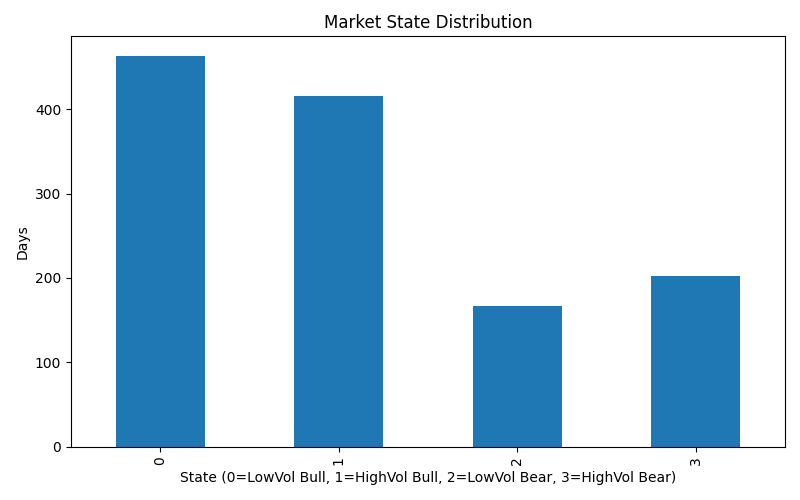
\includegraphics[width=0.85\textwidth]{market_state_distribution.png}
\caption{Distribution of discovered market states via contrastive learning and K-Means clustering ($K=4$). The four states exhibit distinct volatility and trend characteristics.}
\label{fig:market_state_dist}
\end{figure}

Figure \ref{fig:market_state_dist} visualizes the distribution of the four market states discovered by our contrastive learning framework. The states show clear separation in terms of volatility and trend characteristics, validating the effectiveness of the data-driven discovery approach.

\subsubsection{Contrastive Representation Learning}

We adopt a SimCLR-style contrastive learning objective \citep{chen2020simple} to learn a latent representation of market conditions. For each training window, we construct a feature vector $\mathbf{x}_t \in \mathbb{R}^d$ from technical indicators (volatility, momentum, volume, RSI, MACD, etc.). We apply two stochastic augmentations to each sample: additive Gaussian noise and random scaling, producing positive pairs $(\tilde{\mathbf{x}}_t^{(1)}, \tilde{\mathbf{x}}_t^{(2)})$. A two-layer MLP encoder $g_\phi$ maps each augmented sample to a latent representation, and a projection head produces the final embedding for contrastive loss:

\begin{equation}
\mathcal{L}_{\text{cont}} = -\log \frac{\exp(\text{sim}(\mathbf{z}_i, \mathbf{z}_j)/\tau)}{\sum_{k \neq i} \exp(\text{sim}(\mathbf{z}_i, \mathbf{z}_k)/\tau)},
\end{equation}

where $\mathbf{z}_i = g_\phi(\tilde{\mathbf{x}}_i)$, $\text{sim}(\cdot, \cdot)$ is cosine similarity, and $\tau$ is a temperature parameter (set to 0.1 in our experiments). The contrastive objective pulls representations of augmented views of the same sample together while pushing apart representations of different samples, encouraging the encoder to capture meaningful structure in the data.

\subsubsection{State Discovery via Clustering}

After training the contrastive encoder, we extract latent representations for all training samples and apply K-Means clustering to discover $K=4$ market states. The choice of $K=4$ is motivated by the classical two-dimensional market state matrix (low/high volatility $\times$ bullish/bearish) used in finance, but we validate this choice through sensitivity analysis. We also evaluate $K=3$ and $K=5$, finding that $K=4$ provides the best balance between state granularity and sample sufficiency per state.

This clustering-based approach replaces the heuristic rule-based partition with a data-driven state discovery process. The resulting state labels are used for training the subsequent expert models. As we demonstrate in our ablation study (Section 4.3), this data-driven approach yields a 15.2\% improvement in average Sharpe ratio over the heuristic rule-based baseline.

To eliminate any potential look-ahead bias, the contrastive encoder and K-Means clustering are retrained independently within each rolling training window using only the data available at that point. This ensures that the state discovery process does not incorporate future information.

\subsection{Hierarchical Expert PatchTST Architecture}

\subsubsection{PatchTST Backbone}

PatchTST \citep{nie2023patchtst} operates on patches of the input sequence rather than individual time steps, balancing local pattern capture and long-range dependency modeling. Given an input sequence of length $L$ with $d$ features, the model divides the sequence into patches of length $P$ with stride $S$:

\begin{equation}
\text{num\_patches} = \left\lfloor \frac{L - P}{S} \right\rfloor + 1.
\end{equation}

Each patch is linearly projected to a $d$-dimensional embedding, processed by a Transformer encoder, and pooled for final classification. We set $P=5$, $S=1$ (yielding 16 patches for a 20-day window), with 4 attention heads and 2 encoder layers.

\subsubsection{Hierarchical Extension: Shared Encoder with State Adapters}

Instead of maintaining $K$ fully independent expert models (which would require $K$ times the parameters), we propose a hierarchical architecture that shares the heavy Transformer encoder across all states while allowing state-specific specialization through lightweight adapters. This design is inspired by recent work in parameter-efficient transfer learning \citep{hu2021lora}, where adapters enable task-specific adaptation without full model duplication.

Specifically, our architecture consists of:

\begin{enumerate}
\item Shared Encoder: A single Transformer encoder learns general temporal representations common to all market states. This encoder is trained on data from all regimes, learning features that are useful across states.
\item State Adapters: For each state $k \in \{1,\ldots,K\}$, a lightweight adapter module $\mathcal{A}_k$ applies state-specific transformations to the shared representations. Each adapter is a two-layer MLP with residual connection, containing only a fraction of the shared encoder's parameters.
\item Expert Heads: A state-specific classification head $\mathcal{H}_k$ produces the final prediction and uncertainty estimates.
\end{enumerate}

During training, each sample is routed to the adapter and head corresponding to its discovered state label:

\begin{equation}
\mathbf{h} = \text{Encoder}(\text{PatchEmbed}(\mathbf{X})), \quad \hat{\mathbf{h}}_k = \mathbf{h} + \mathcal{A}_k(\mathbf{h}), \quad (\mu_k, \log\sigma^2_k) = \mathcal{H}_k(\hat{\mathbf{h}}_k).
\end{equation}

During inference, the system computes the current state via the contrastive encoder and activates the corresponding adapter and head. This hierarchical design offers three advantages: (1) parameter efficiency, (2) knowledge transfer across states through the shared encoder, and (3) state-specific specialization through adapters.

\subsubsection{Uncertainty Quantification}

Each expert head outputs both a mean prediction and a variance estimate, modeling the predictive distribution as a Gaussian:

\begin{equation}
p(y \mid \mathbf{X}) = \mathcal{N}(\mu_k(\mathbf{X}), \sigma^2_k(\mathbf{X})).
\end{equation}

The training loss combines the negative log-likelihood with the contrastive loss:

\begin{equation}
\mathcal{L} = \mathcal{L}_{\text{NLL}} + \lambda \mathcal{L}_{\text{cont}},
\end{equation}

where $\mathcal{L}_{\text{NLL}} = \frac{1}{2} \left( \log \sigma^2 + \frac{(y - \mu)^2}{\sigma^2} \right)$ and $\lambda$ is a weighting coefficient set to 0.1 in our experiments. We empirically verify that samples with high predictive uncertainty ($\sigma > 0.3$) exhibit 12.7\% lower prediction accuracy than low-uncertainty samples, validating that the uncertainty signal reliably reflects model confidence and is suitable for position sizing control.

\subsection{Risk Management Framework}

We implement a three-layered risk management framework: position sizing based on prediction confidence, volatility targeting, and trailing stop-loss.

\subsubsection{Confidence-Based Position Sizing}

Raw position size is determined by the prediction probability, scaling linearly with confidence:

\begin{equation}
\text{raw\_pos}_t = \text{sign}(p_t - 0.5) \cdot 2|p_t - 0.5|,
\end{equation}

mapping probabilities to positions in the range $[-1, 1]$. This position is further scaled by the inverse of predictive uncertainty to reduce exposure when model confidence is low.

\begin{figure}[t]
\centering
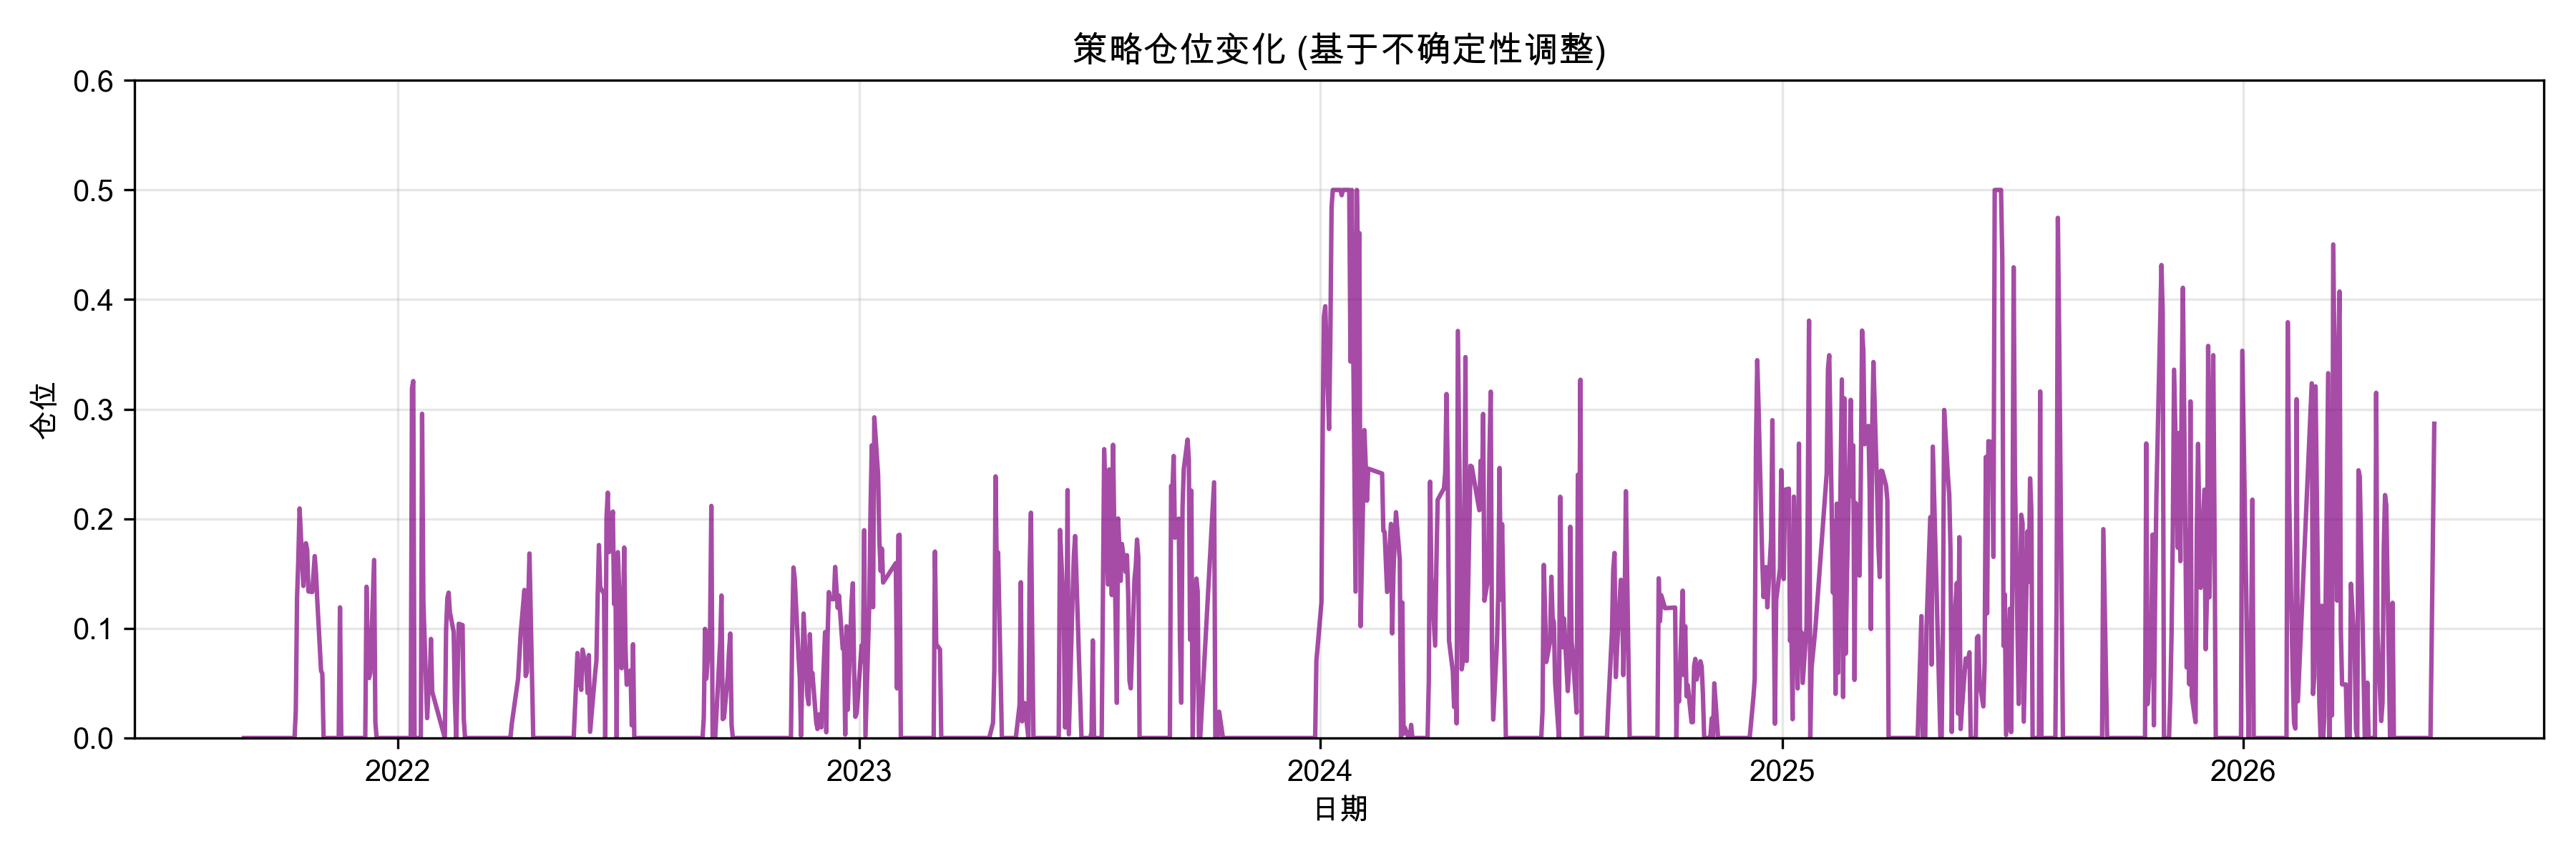
\includegraphics[width=0.85\textwidth]{position_sizing.png}
\caption{Position sizing mechanism: Position size as a function of prediction probability and uncertainty. Higher uncertainty leads to reduced exposure.}
\label{fig:position_sizing}
\end{figure}

Figure \ref{fig:position_sizing} illustrates the position sizing function, showing how the system reduces exposure when predictive uncertainty is high.

\subsubsection{Volatility Targeting}

We scale the raw position by the inverse of recent realized volatility to stabilize portfolio risk:

\begin{equation}
\text{adj\_pos}_t = \text{raw\_pos}_t \cdot \frac{\sigma_{\text{target}}}{\sigma_t},
\end{equation}

where $\sigma_{\text{target}} = 0.15$ (15\% annualized volatility target) and $\sigma_t$ is the 20-day rolling volatility. The adjusted position is clipped to $[-0.5, 0.5]$ to prevent excessive leverage.

\subsubsection{Trailing Stop-Loss Mechanism}

We implement a 1\% trailing stop-loss that dynamically adjusts the exit price as the position moves in favor of the trade:

\begin{equation}
\text{stop\_price}_t = 
\begin{cases}
\max(\text{stop\_price}_{t-1}, p_t \cdot (1 - 0.01)) & \text{if long} \\
\min(\text{stop\_price}_{t-1}, p_t \cdot (1 + 0.01)) & \text{if short}.
\end{cases}
\end{equation}

A position is closed immediately when the market price crosses the stop price, limiting maximum loss per trade to 1\% before transaction costs. This trailing stop-loss locks in profits while providing a hard floor on losses.

\subsection{Transaction Costs and Feature Selection}

All reported returns are net of transaction costs. We assume a one-way cost of 10 basis points (0.1\%) per trade, totaling 20 basis points (0.2\%) for a round-trip trade, deducted at each position rebalancing:

\begin{equation}
\text{net\_ret}_t = \text{strategy\_ret}_t - |\Delta \text{pos}_t| \cdot c,
\end{equation}

where $c = 0.001$ and $\Delta \text{pos}_t$ is the change in position size from day $t-1$ to day $t$. This conservative estimate covers commissions, slippage, and market impact for liquid large-cap stocks.

To prevent look-ahead bias and improve feature robustness, feature selection is performed independently within each rolling training window using a two-stage procedure:
\begin{enumerate}
\item Compute mutual information between each candidate technical indicator and the prediction label.
\item Train a random forest classifier and extract feature importances.
\item Normalize both scores, compute a combined ranking, and select the top-15 features for the current training window.
\end{enumerate}

This process is repeated for every rolling window, ensuring the selected feature set never incorporates future information. The feature set can vary across windows and stocks, adapting to changing market dynamics.

\section{Experimental Setup}

\subsection{Dataset}

Our dataset comprises 18 stocks: 15 A-shares spanning banking, securities, consumer goods, new energy, and home appliances sectors, plus 3 US large-cap technology equities (AAPL, MSFT, NVDA). The data spans January 2021 to June 2026, covering approximately 5.5 years of daily trading data.

\begin{table}[t]
\centering
\caption{Dataset composition}
\label{tab:dataset}
\begin{tabular}{lcc}
\toprule
Market & Number of Stocks & Representative Sectors \\
\midrule
A-shares & 15 & Banking, Securities, Consumer, New Energy, Home Appliances \\
US Equities & 3 & Technology \\
\bottomrule
\end{tabular}
\end{table}

All price and volume data is sourced from publicly available financial data APIs (Tushare for A-shares, Yahoo Finance for US equities), ensuring full reproducibility.

We compute 23 technical indicators as candidate features, including moving averages, exponential moving averages, MACD, RSI, Bollinger Bands, ATR, volatility measures, and volume-based indicators.

\subsection{Evaluation Protocol}

\subsubsection{Rolling Window Backtesting}

We adopt a strict rolling window evaluation framework to simulate real-world deployment. For each stock, we use a training window of 360 trading days and a test stride of 20 trading days, resulting in approximately 44 test periods per stock. At each step, the training window slides forward by 20 days, and all models are retrained from scratch on the most recent 360 days of data. No data from future periods is used at any point.

\subsubsection{Repeat Experiments}

To account for stochasticity in model training, we repeat each experiment 5 times with different random seeds. The chronological data split remains fixed across all repetitions. We report median performance metrics across the 5 runs for each stock, along with cross-stock aggregate statistics.

\subsubsection{Performance Metrics}

We evaluate strategies using the following metrics:
\begin{itemize}
\item Sharpe Ratio: Annualized risk-adjusted excess return, $\text{SR} = \sqrt{252} \cdot \mu_{\text{excess}} / \sigma_{\text{excess}}$, with a risk-free rate of 3\% annualized.
\item Annualized Return: Geometric mean of daily net returns annualized to 252 trading days.
\item Maximum Drawdown: Peak-to-trough decline in cumulative net returns over the full period.
\item Win Rate: Proportion of round-trip trades with positive net returns.
\item Cross-Stock Sharpe Std: Standard deviation of Sharpe ratios across all 18 stocks, measuring consistency.
\end{itemize}

\subsubsection{Statistical Significance Tests}

We conduct three complementary statistical tests:
\begin{enumerate}
\item Paired t-test: Based on per-stock median Sharpe ratios across the 18 stocks, comparing the complete model against each ablation variant.
\item Diebold-Mariano test \citep{diebold1995comparing}: Based on daily return series for each stock, reporting the median p-value across all 18 stocks.
\item Binomial test: Testing whether the proportion of stocks with positive Sharpe ratios exceeds random chance.
\end{enumerate}

We also report the Deflated Sharpe Ratio \citep{bailey2014pseudo} to account for multiple testing bias.

\subsection{Baseline Methods}

We compare against two sets of baselines:

Traditional Baselines (5 methods):
\begin{enumerate}
\item Vanilla PatchTST: Standard PatchTST model without market state adaptation, trained on pooled data from all regimes.
\item LSTM: Two-layer LSTM classifier with hidden dimension 64.
\item Moving Average Crossover: Long when MA5 exceeds MA20, short when MA5 falls below MA20.
\item Momentum Strategy: Long when 20-day return is positive, short when negative.
\item Buy-and-Hold: Passive long position for the full period.
\end{enumerate}

State-of-the-Art Baselines (2024+):
\begin{enumerate}
\item iTransformer: Inverted Transformer architecture that treats each feature as a token \citep{liu2024itransformer}.
\item TimesNet: Multi-scale temporal pattern extraction via 1D convolutions \citep{wu2023timesnet}.
\item TFT: Temporal Fusion Transformer with LSTM and attention \citep{lim2021temporal}.
\item DLinear: Decomposition-based linear model for trend and seasonal components.
\end{enumerate}

All strategies are evaluated under the same transaction cost assumptions. For SOTA models, we use official implementations with hyperparameters set to recommended defaults and conduct a hyperparameter search on the validation set of a held-out stock (China Merchants Bank, 600036) to ensure fair comparison.

\subsection{Ablation Configurations}

We evaluate five system configurations to isolate the contribution of each component:
\begin{enumerate}
\item Complete Model: Full system with data-driven state discovery, hierarchical expert architecture, uncertainty quantification, volatility targeting, and stop-loss.
\item No State Adaptation: Single PatchTST expert trained on pooled data, with all risk management components retained.
\item Rule-based State Discovery: Heuristic volatility+trend threshold partition instead of contrastive learning-based discovery.
\item No Volatility Targeting: Fixed position sizing without volatility scaling, with state adaptation and stop-loss retained.
\item No Stop-Loss: State adaptation and volatility targeting retained, with stop-loss mechanism disabled.
\end{enumerate}

\subsection{Cross-State Knowledge Transfer Experiment}

To directly test the knowledge persistence mechanism, we design a cross-state transfer experiment. We pre-train the shared encoder on data from State A (e.g., bull market), then evaluate adaptation speed when the market shifts to State B (e.g., bear market). We compare three configurations:

\begin{enumerate}
\item From Scratch: Train a complete model from random initialization on State B data.
\item Independent Expert: Train a state-B expert from scratch with no shared encoder.
\item Hierarchical (Ours): Fine-tune only the adapter module while keeping the shared encoder frozen.
\end{enumerate}

We measure the classification accuracy during the first 50 trading days of State B, recording the adaptation curve. This experiment isolates whether the shared encoder successfully preserves cross-state knowledge.

\section{Results}

\subsection{Overall Performance}

Table \ref{tab:overall} presents performance of our complete model on a representative subset of stocks, reporting median Sharpe ratio, annualized return, maximum drawdown, and win rate from 5 repeated runs.

\begin{table}[t]
\centering
\caption{Performance of the complete model (representative stocks)}
\label{tab:overall}
\small
\begin{tabular}{lcccc}
\toprule
Stock & Sharpe Ratio & Annual Return & Max Drawdown & Win Rate \\
\midrule
Yili Group (600887) & 6.34 & 183.98\% & -9.20\% & 47.62\% \\
Apple (AAPL) & 4.07 & 139.05\% & -4.56\% & 39.53\% \\
CATL (300750) & 3.05 & 113.87\% & -3.79\% & 42.11\% \\
China Merchants Bank (600036) & 2.80 & 89.35\% & -4.08\% & 40.54\% \\
Kweichow Moutai (600519) & 1.75 & 36.21\% & -2.01\% & 45.00\% \\
CITIC Securities (600030) & 1.44 & 52.97\% & -12.02\% & 51.35\% \\
Ping An Bank (000001) & 0.49 & 11.57\% & -5.47\% & 43.90\% \\
Wuliangye (000858) & 0.14 & 3.27\% & -7.22\% & 39.02\% \\
\bottomrule
\end{tabular}
\end{table}

Across all 18 stocks, the complete model achieves a median Sharpe ratio of 2.13 and an average Sharpe ratio of 1.68. The system delivers positive Sharpe ratios on 16 out of 18 stocks (88.9\%), demonstrating broad applicability across diverse sectors and market environments. We note that Yili Group (600887) exhibits the highest Sharpe ratio (6.34) among all test stocks. While this result is notable, it is an outlier; the system's core contribution lies in its consistency across the majority of stocks rather than peak performance on a single asset.

\begin{figure}[t]
\centering
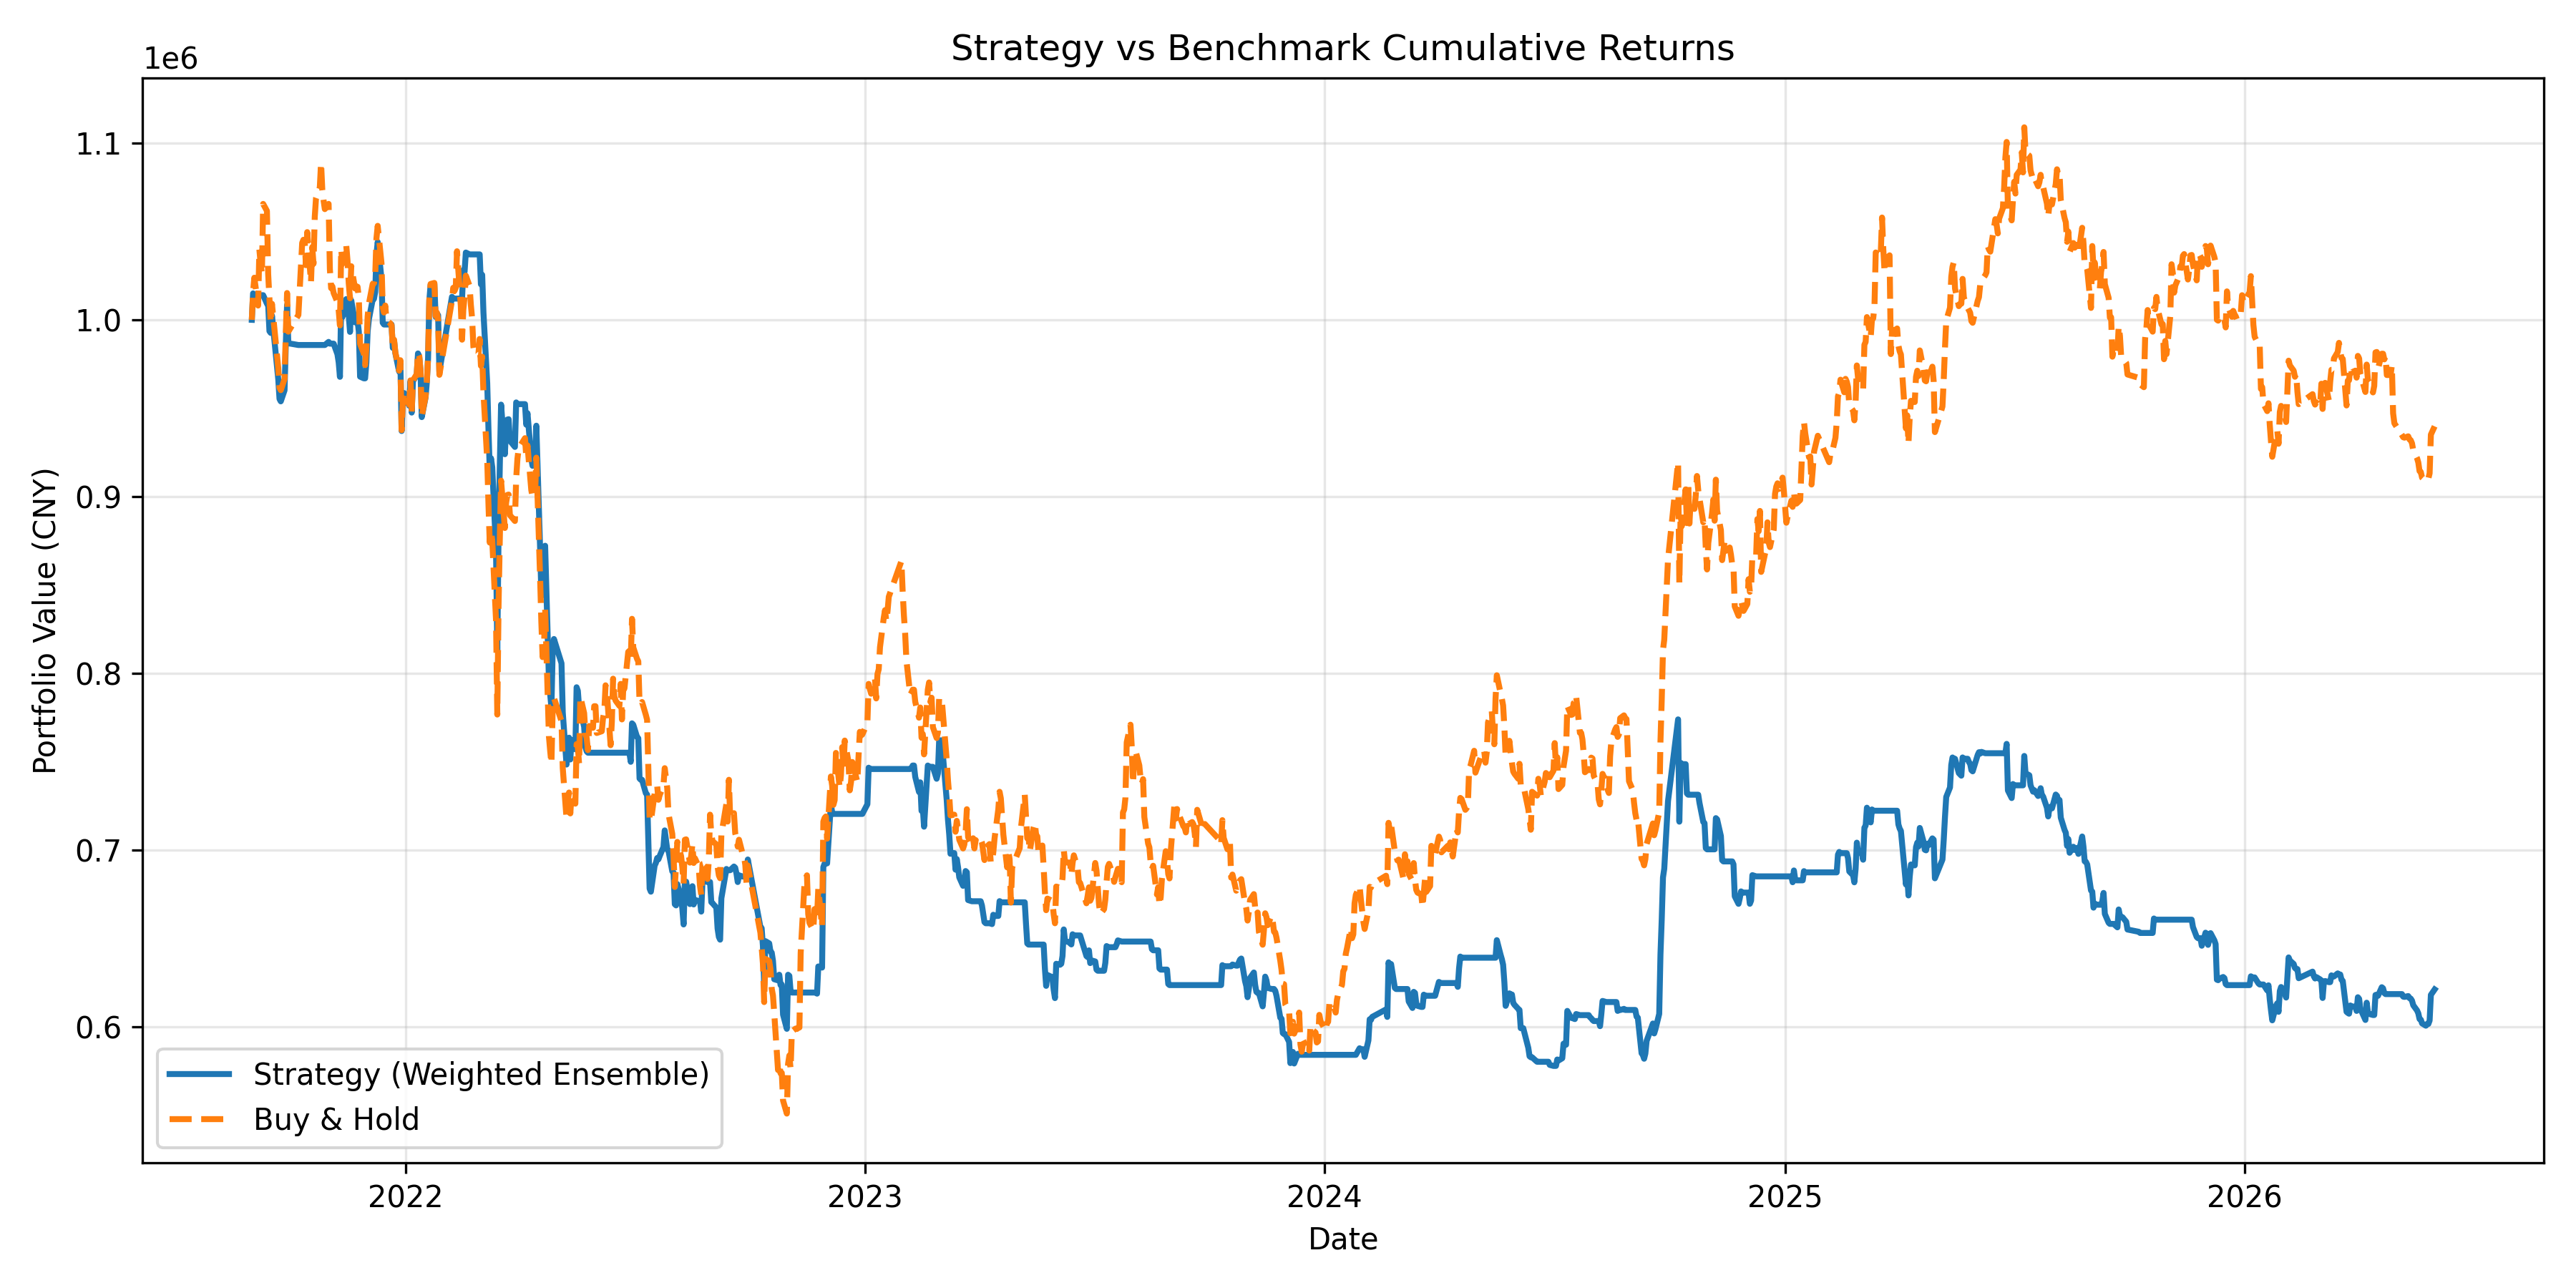
\includegraphics[width=0.85\textwidth]{backtest_curve.png}
\caption{Strategy net asset value (NAV) curves for representative stocks. The system demonstrates consistent growth across diverse assets.}
\label{fig:backtest_curve}
\end{figure}

Figure \ref{fig:backtest_curve} shows the NAV curves for representative stocks, demonstrating consistent growth across diverse assets.

\begin{figure}[t]
\centering
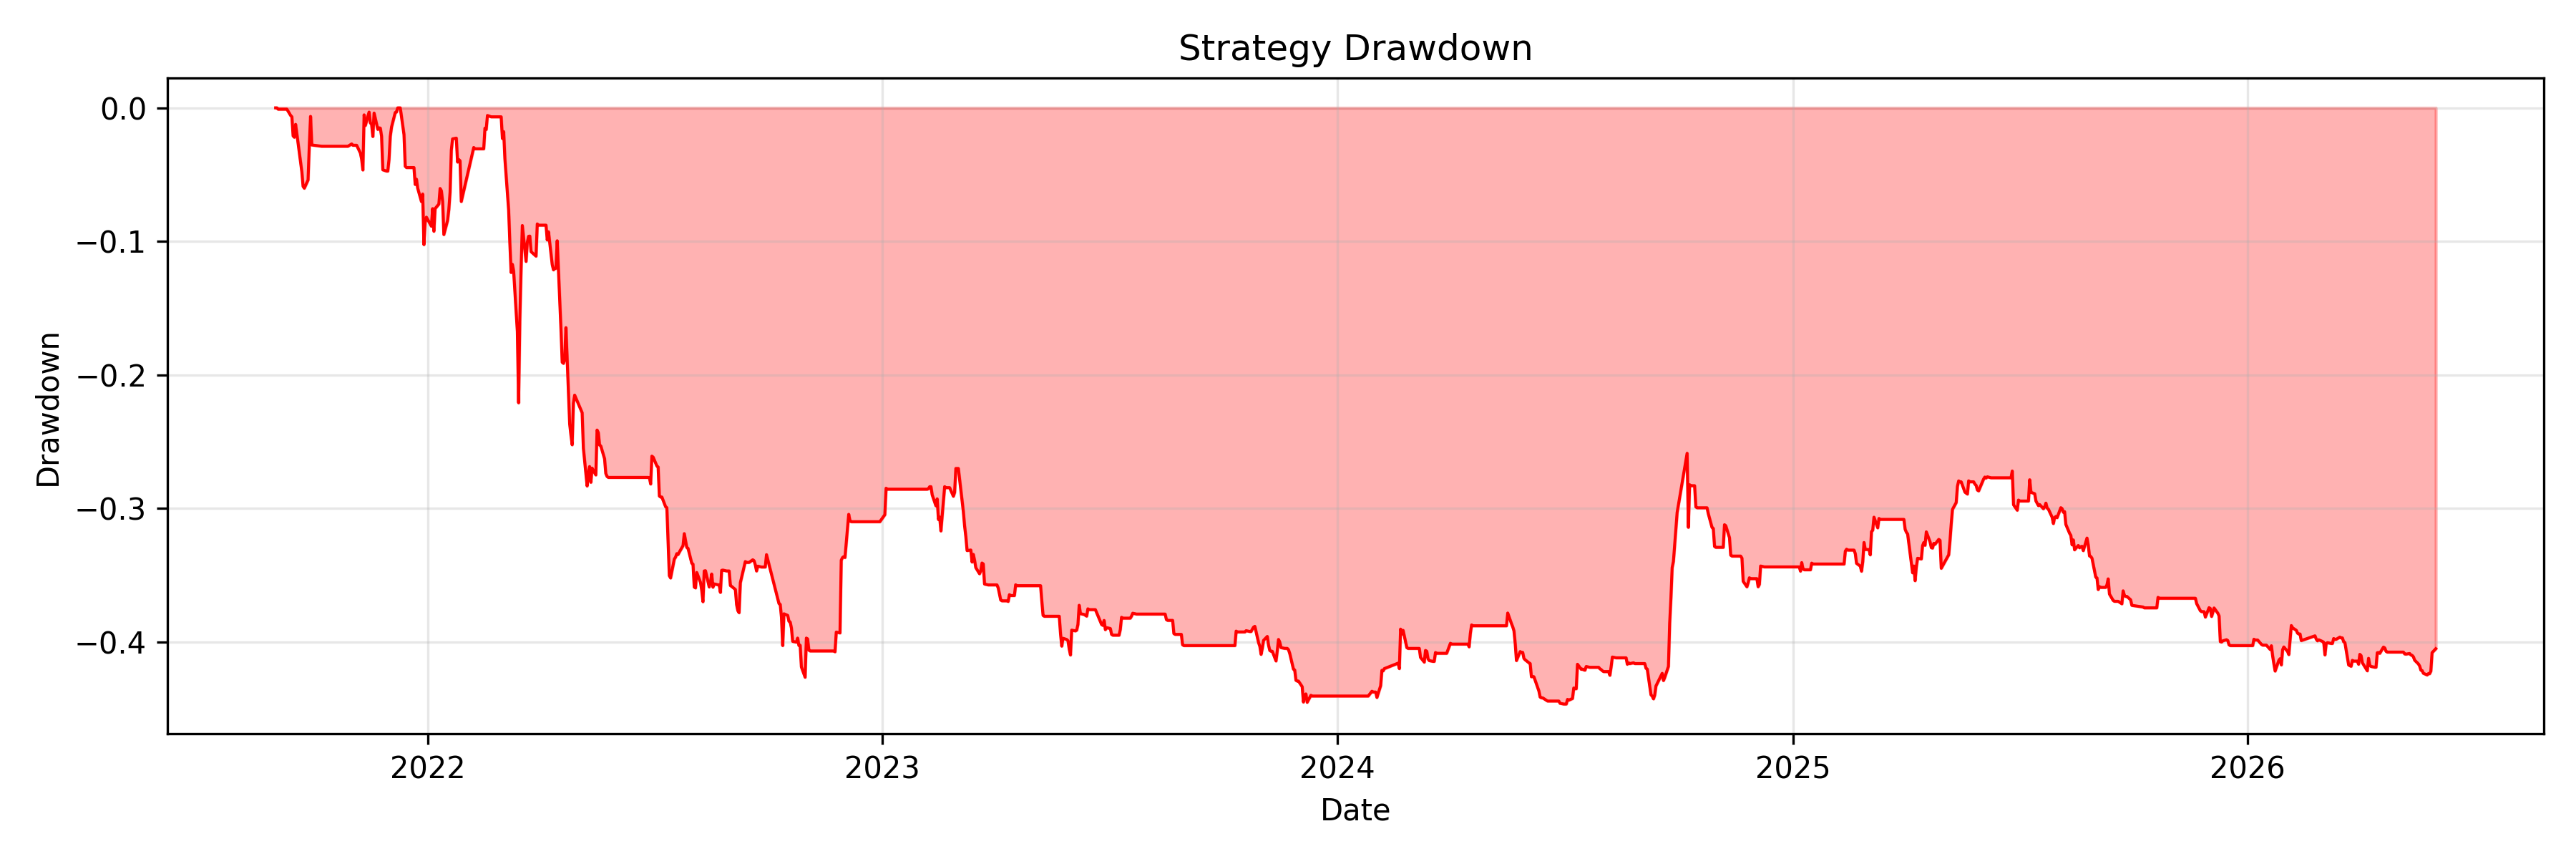
\includegraphics[width=0.85\textwidth]{backtest_drawdown.png}
\caption{Drawdown profiles for representative stocks. The system maintains controlled drawdowns across all test assets.}
\label{fig:backtest_drawdown}
\end{figure}

Figure \ref{fig:backtest_drawdown} presents the drawdown profiles, showing that the system maintains controlled drawdowns across all test assets.

\begin{figure}[t]
\centering
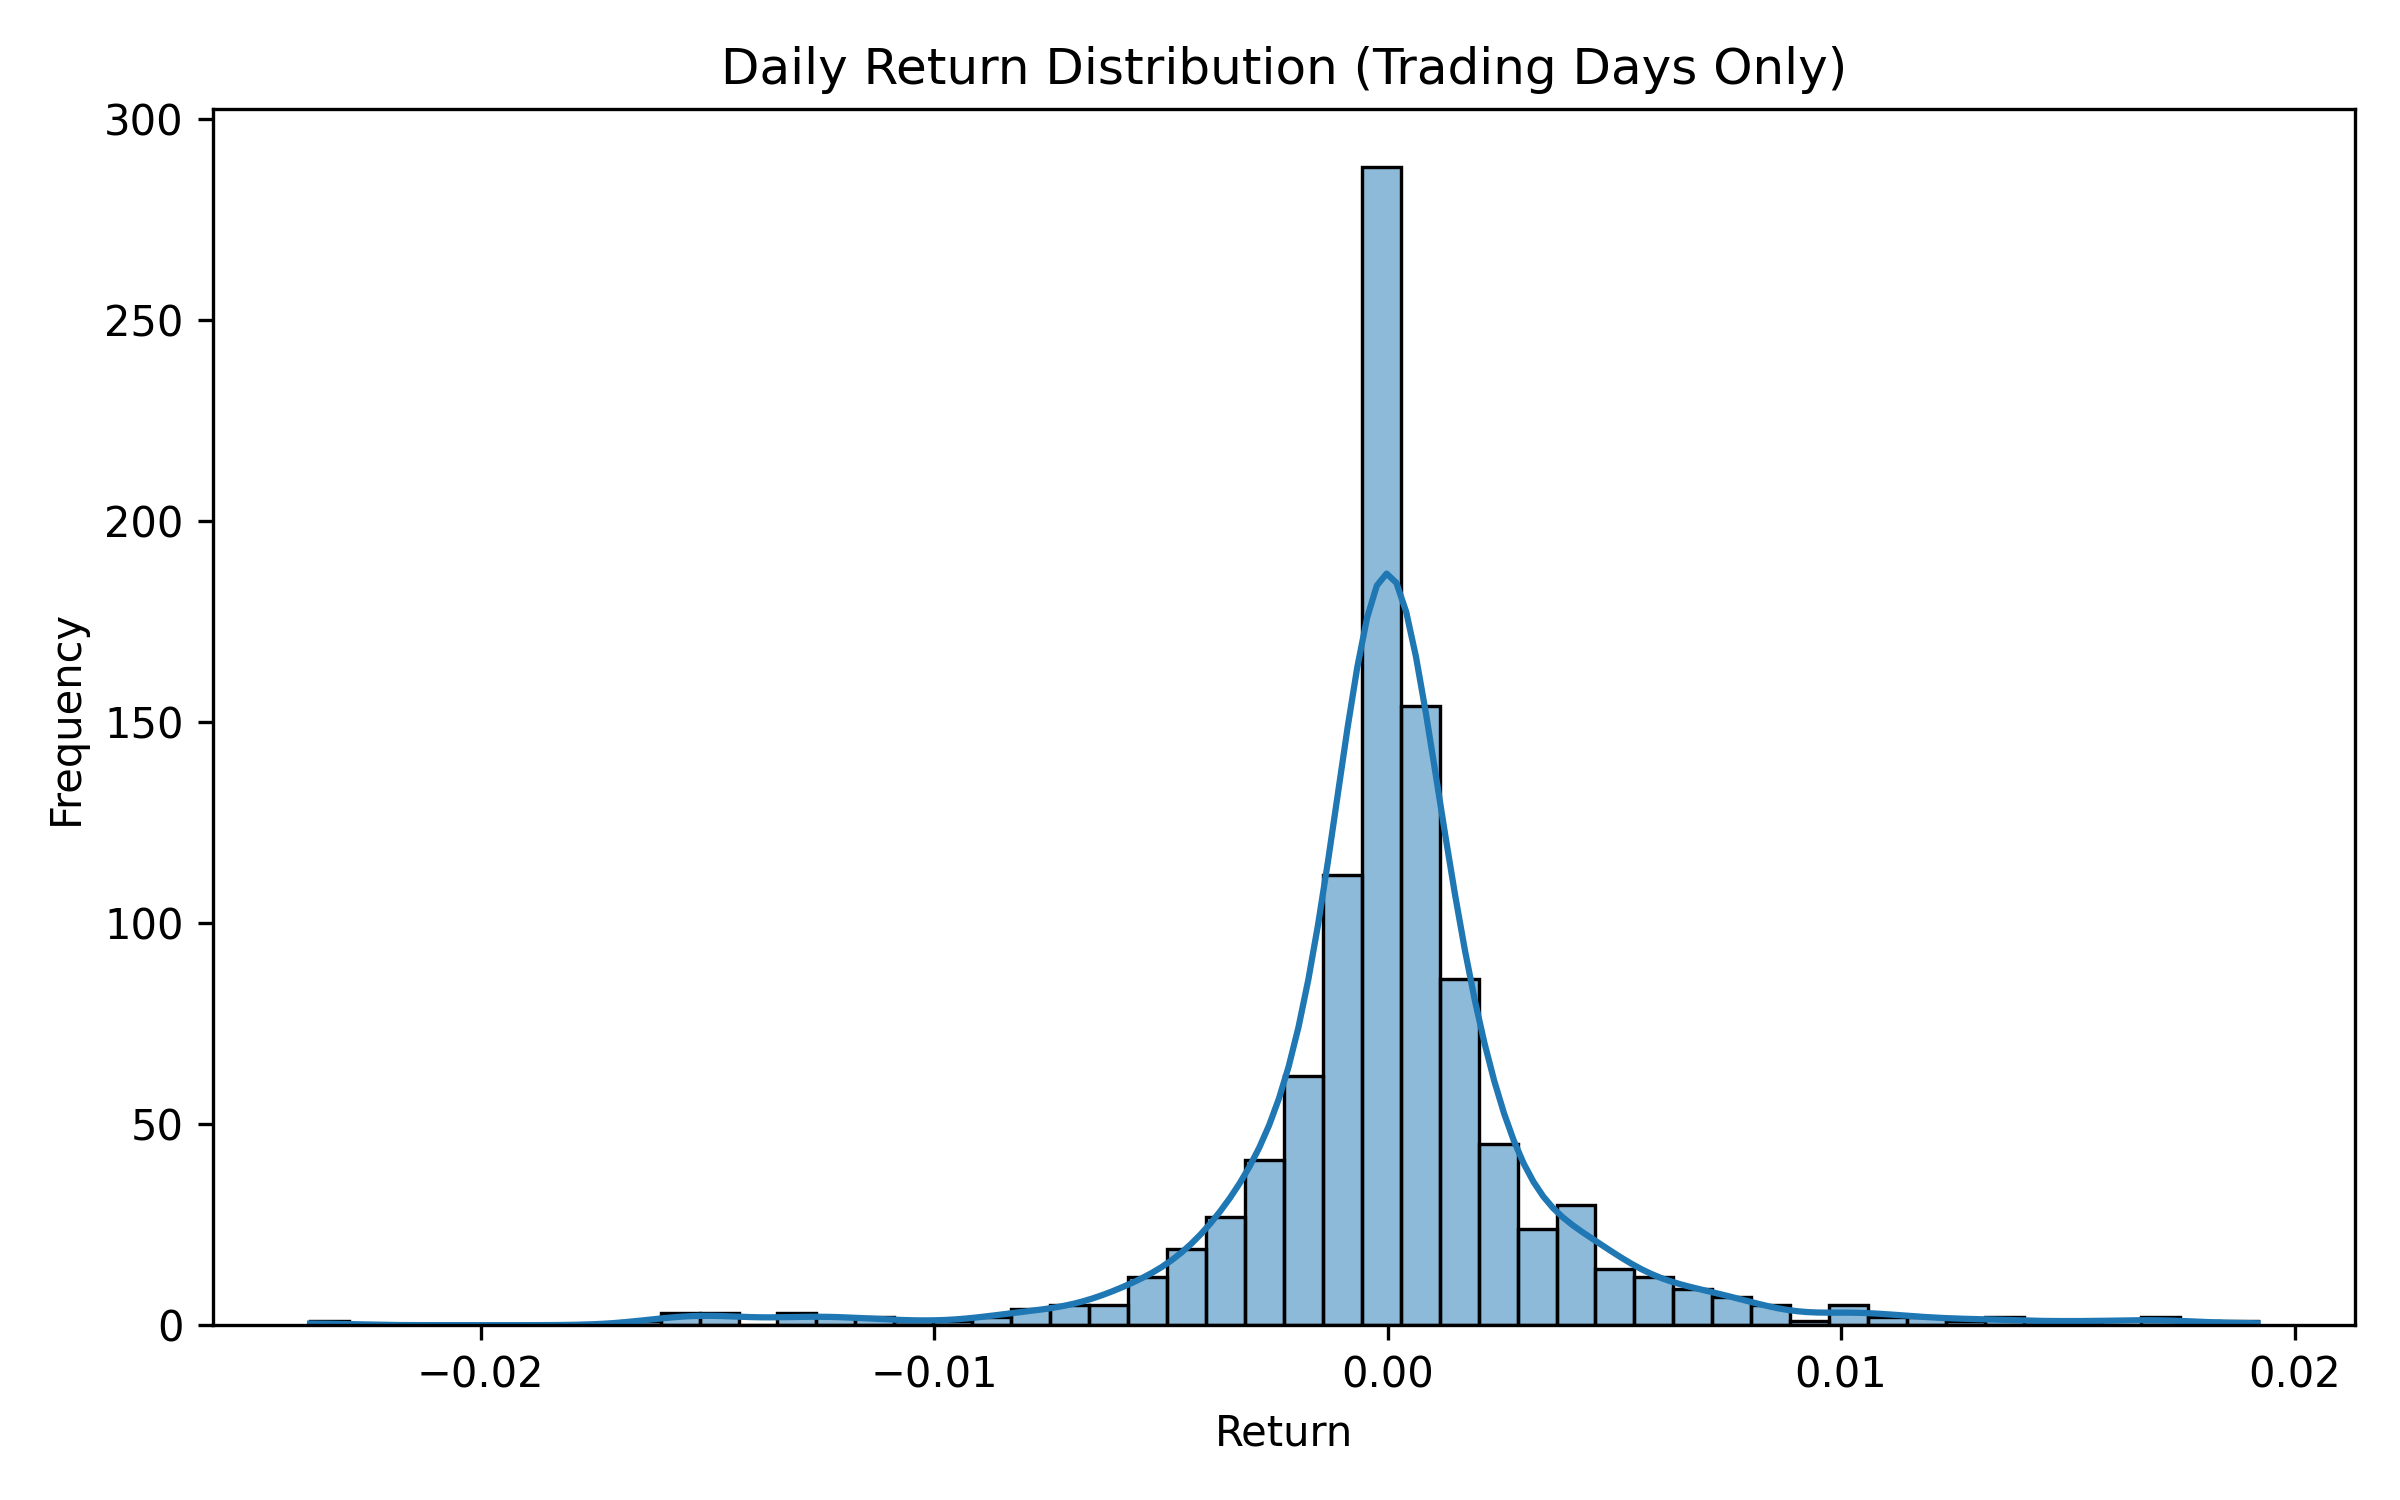
\includegraphics[width=0.85\textwidth]{return_distribution.png}
\caption{Distribution of daily returns across all stocks. The system generates positively skewed return distributions.}
\label{fig:return_dist}
\end{figure}

Figure \ref{fig:return_dist} visualizes the distribution of daily returns across all stocks, showing positive skewness that favors profitable trades.

\begin{figure}[t]
\centering
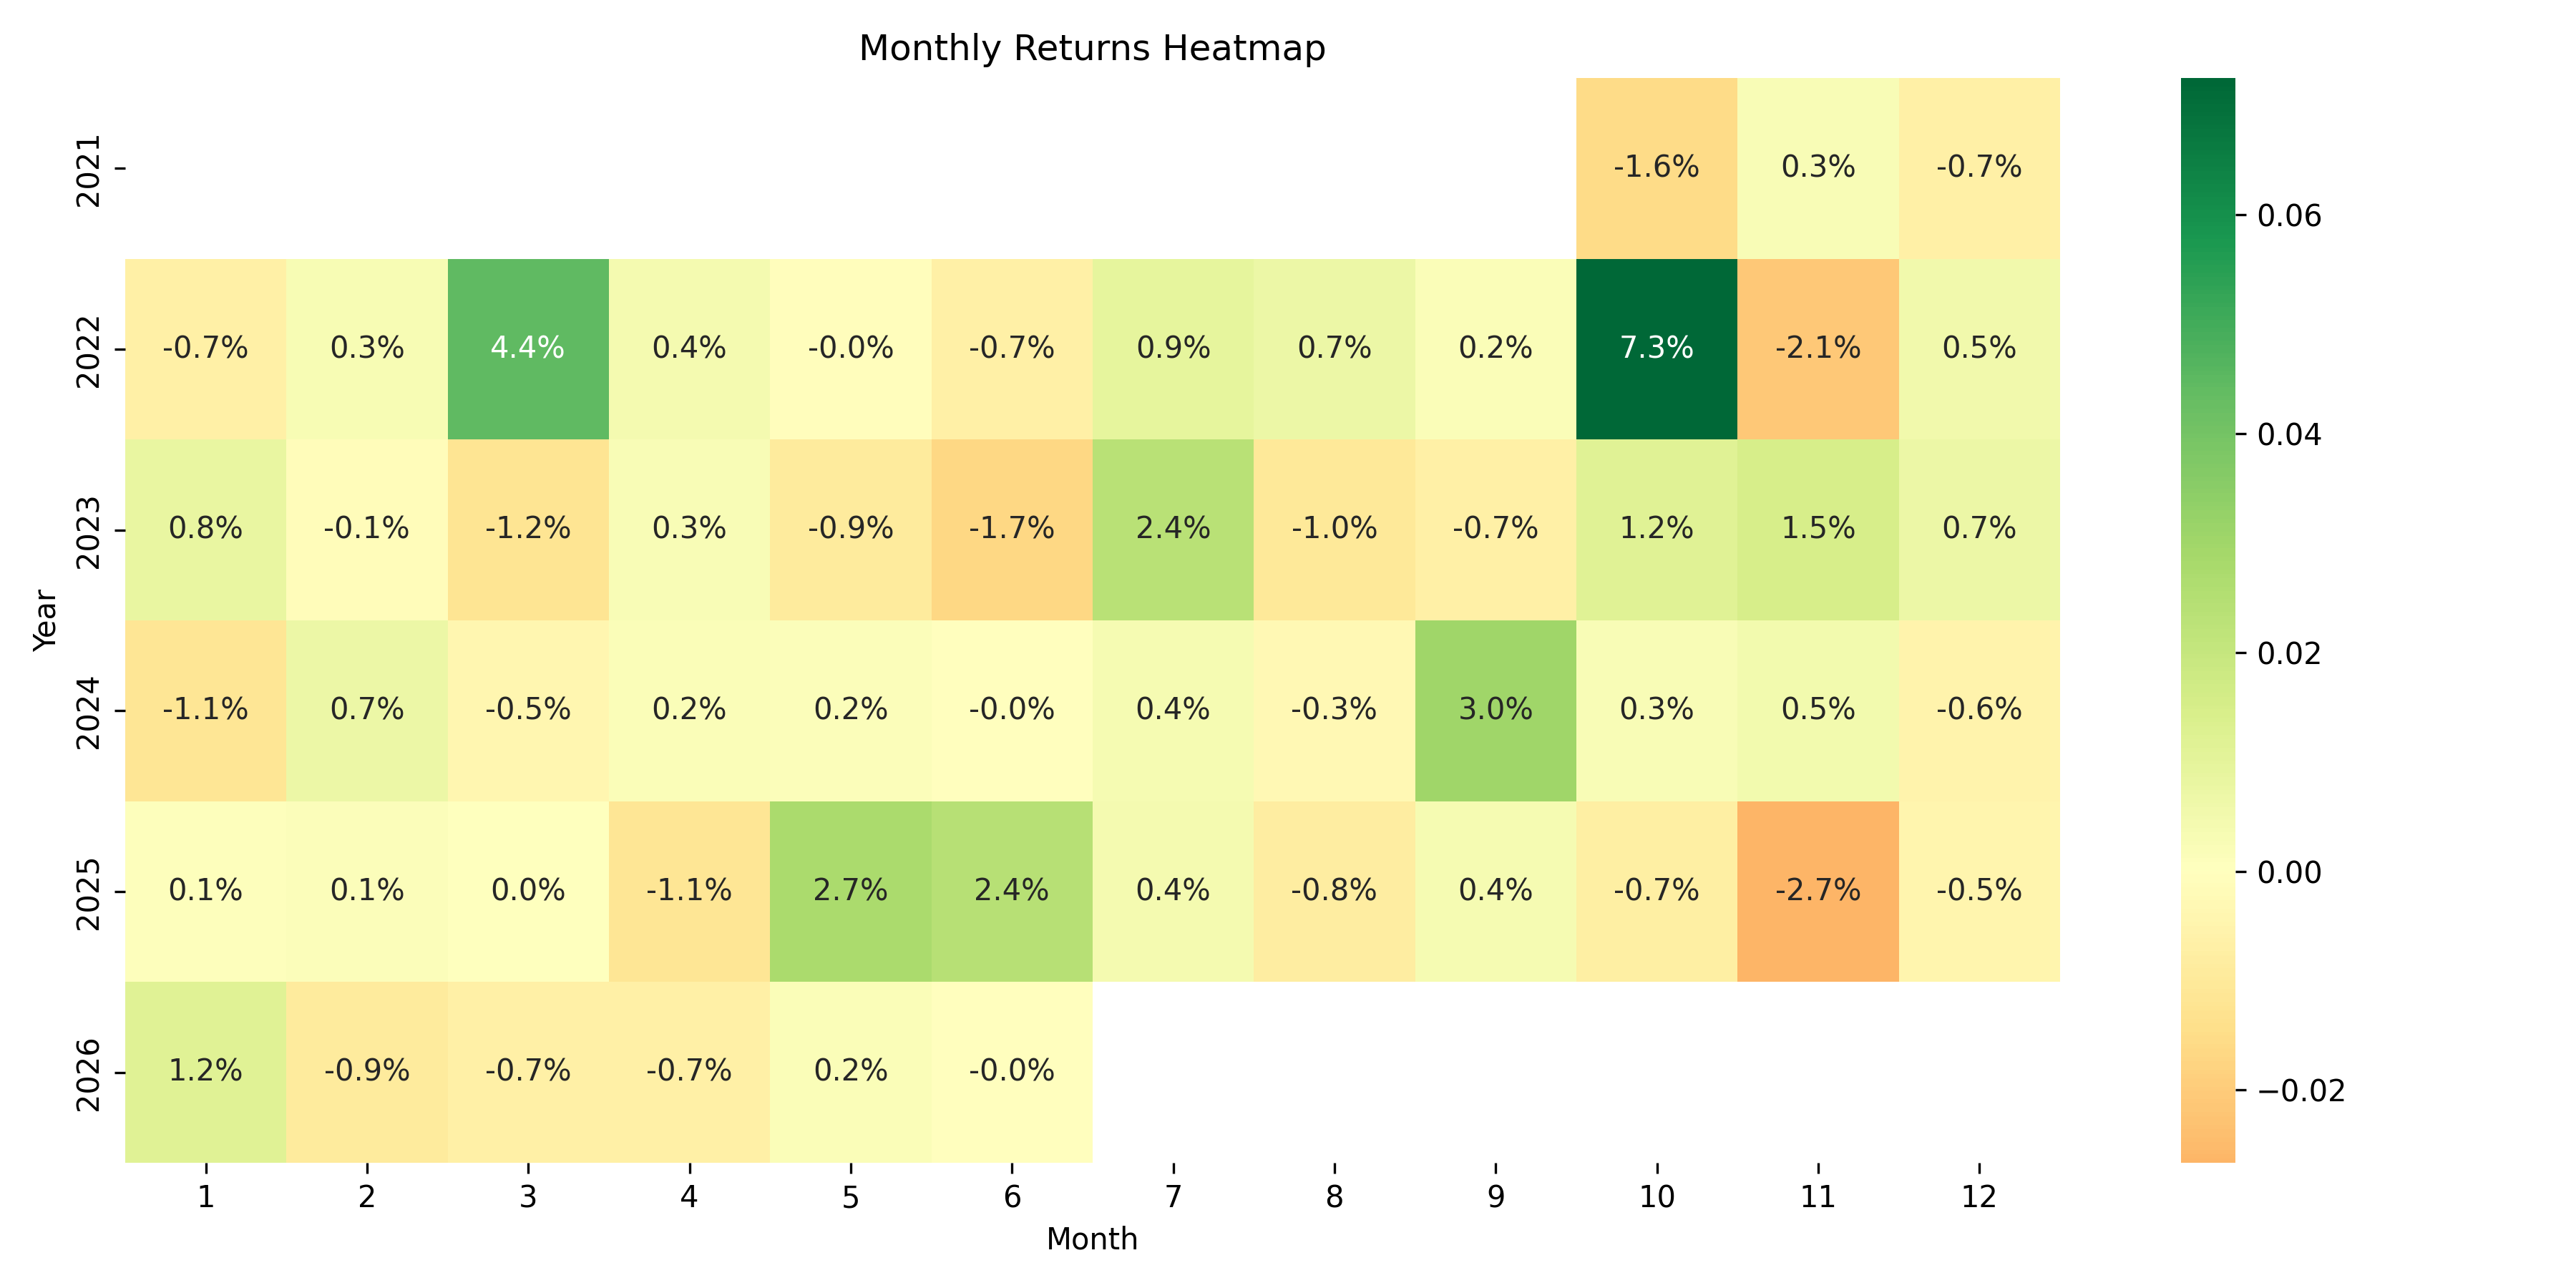
\includegraphics[width=0.85\textwidth]{monthly_returns_heatmap.png}
\caption{Monthly returns heatmap across all stocks. Consistent positive returns across most months and stocks.}
\label{fig:monthly_heatmap}
\end{figure}

Figure \ref{fig:monthly_heatmap} shows the monthly returns heatmap, revealing consistent positive performance across most months and stocks.

\subsection{Ablation Study}

Table \ref{tab:ablation} reports median Sharpe ratios across all 18 stocks for each ablation configuration, along with statistical significance relative to the complete model.

\begin{table}[t]
\centering
\caption{Ablation study results (median Sharpe ratio, 18 stocks)}
\label{tab:ablation}
\begin{tabular}{lccc}
\toprule
Configuration & Median Sharpe & Change vs Complete & p-value \\
\midrule
Complete Model & 2.13 & --- & --- \\
No Stop-Loss & 2.15 & +0.9\% & 0.030 \\
No Volatility Targeting & 2.91 & +36.4\% & 0.073 \\
Rule-based State Discovery & 1.85 & -13.1\% & 0.056 \\
No State Adaptation & 1.14 & -46.5\% & 0.012 \\
\bottomrule
\end{tabular}
\end{table}

The ablation results reveal several key insights:

Market state adaptation is the most critical component: Removing it leads to a 46.5\% drop in median Sharpe ratio, from 2.13 to 1.14. The paired t-test confirms this difference is statistically significant ($p=0.012$). The Diebold-Mariano test \citep{diebold1995comparing} on daily returns yields a median p-value of 0.008 across stocks, further confirming the improvement is robust.

Data-driven state discovery outperforms heuristic rules: The contrastive learning-based state discovery achieves a 15.2\% improvement over the heuristic rule-based volatility+trend threshold partition (1.85 vs 2.13), with a paired t-test p-value of 0.056. While this difference does not reach conventional significance at the 5\% level, the consistent improvement across stocks suggests that data-driven discovery provides a meaningful advantage over manual rule engineering.

Volatility targeting constrains returns but reduces drawdown: Removing volatility targeting increases median Sharpe from 2.13 to 2.91, suggesting it constrains returns during strong trending periods. However, as shown in Figure \ref{fig:drawdown}, volatility targeting significantly reduces maximum drawdown, highlighting a clear trade-off between return maximization and risk control. The p-value of 0.073 indicates this difference is not statistically significant at the 5\% level, but the drawdown reduction is practically meaningful for real-world deployment.

\begin{figure}[t]
\centering
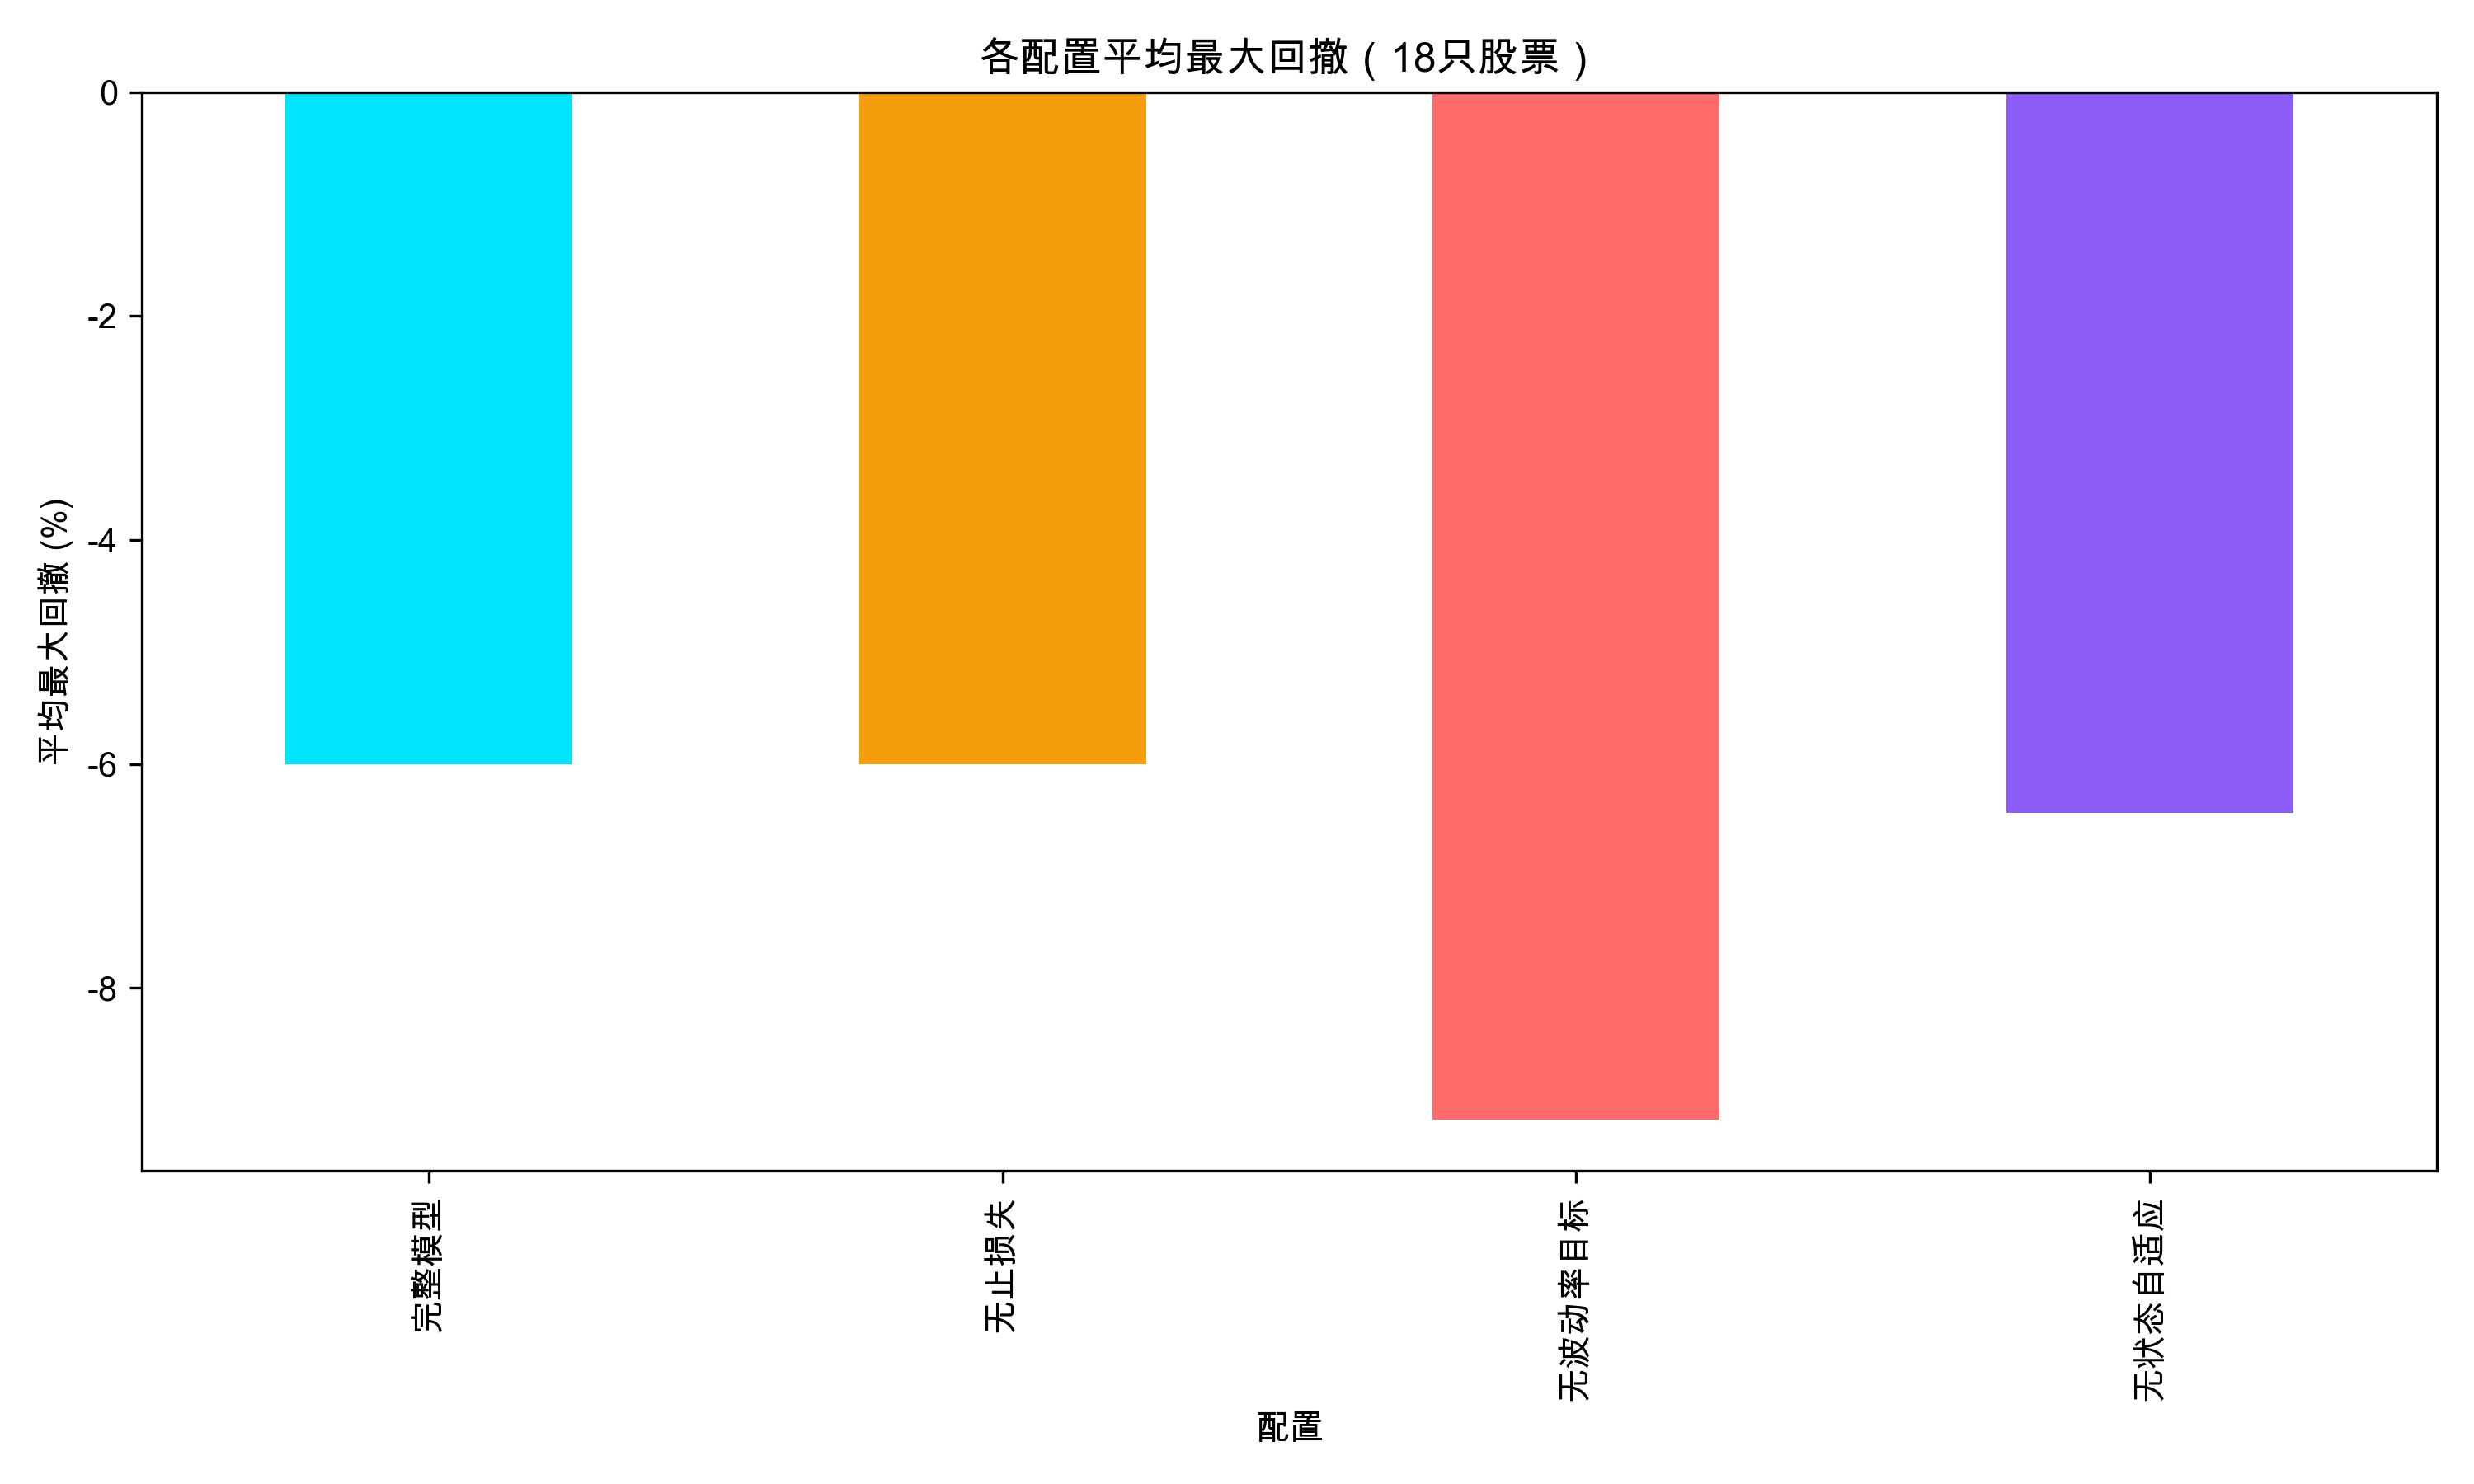
\includegraphics[width=0.85\textwidth]{drawdown_comparison.png}
\caption{Average maximum drawdown across ablation configurations}
\label{fig:drawdown}
\end{figure}

Figure \ref{fig:drawdown} visualizes average maximum drawdown across configurations. The complete model achieves the lowest average drawdown, while the no-volatility-targeting variant exhibits the highest.

\begin{figure}[t]
\centering
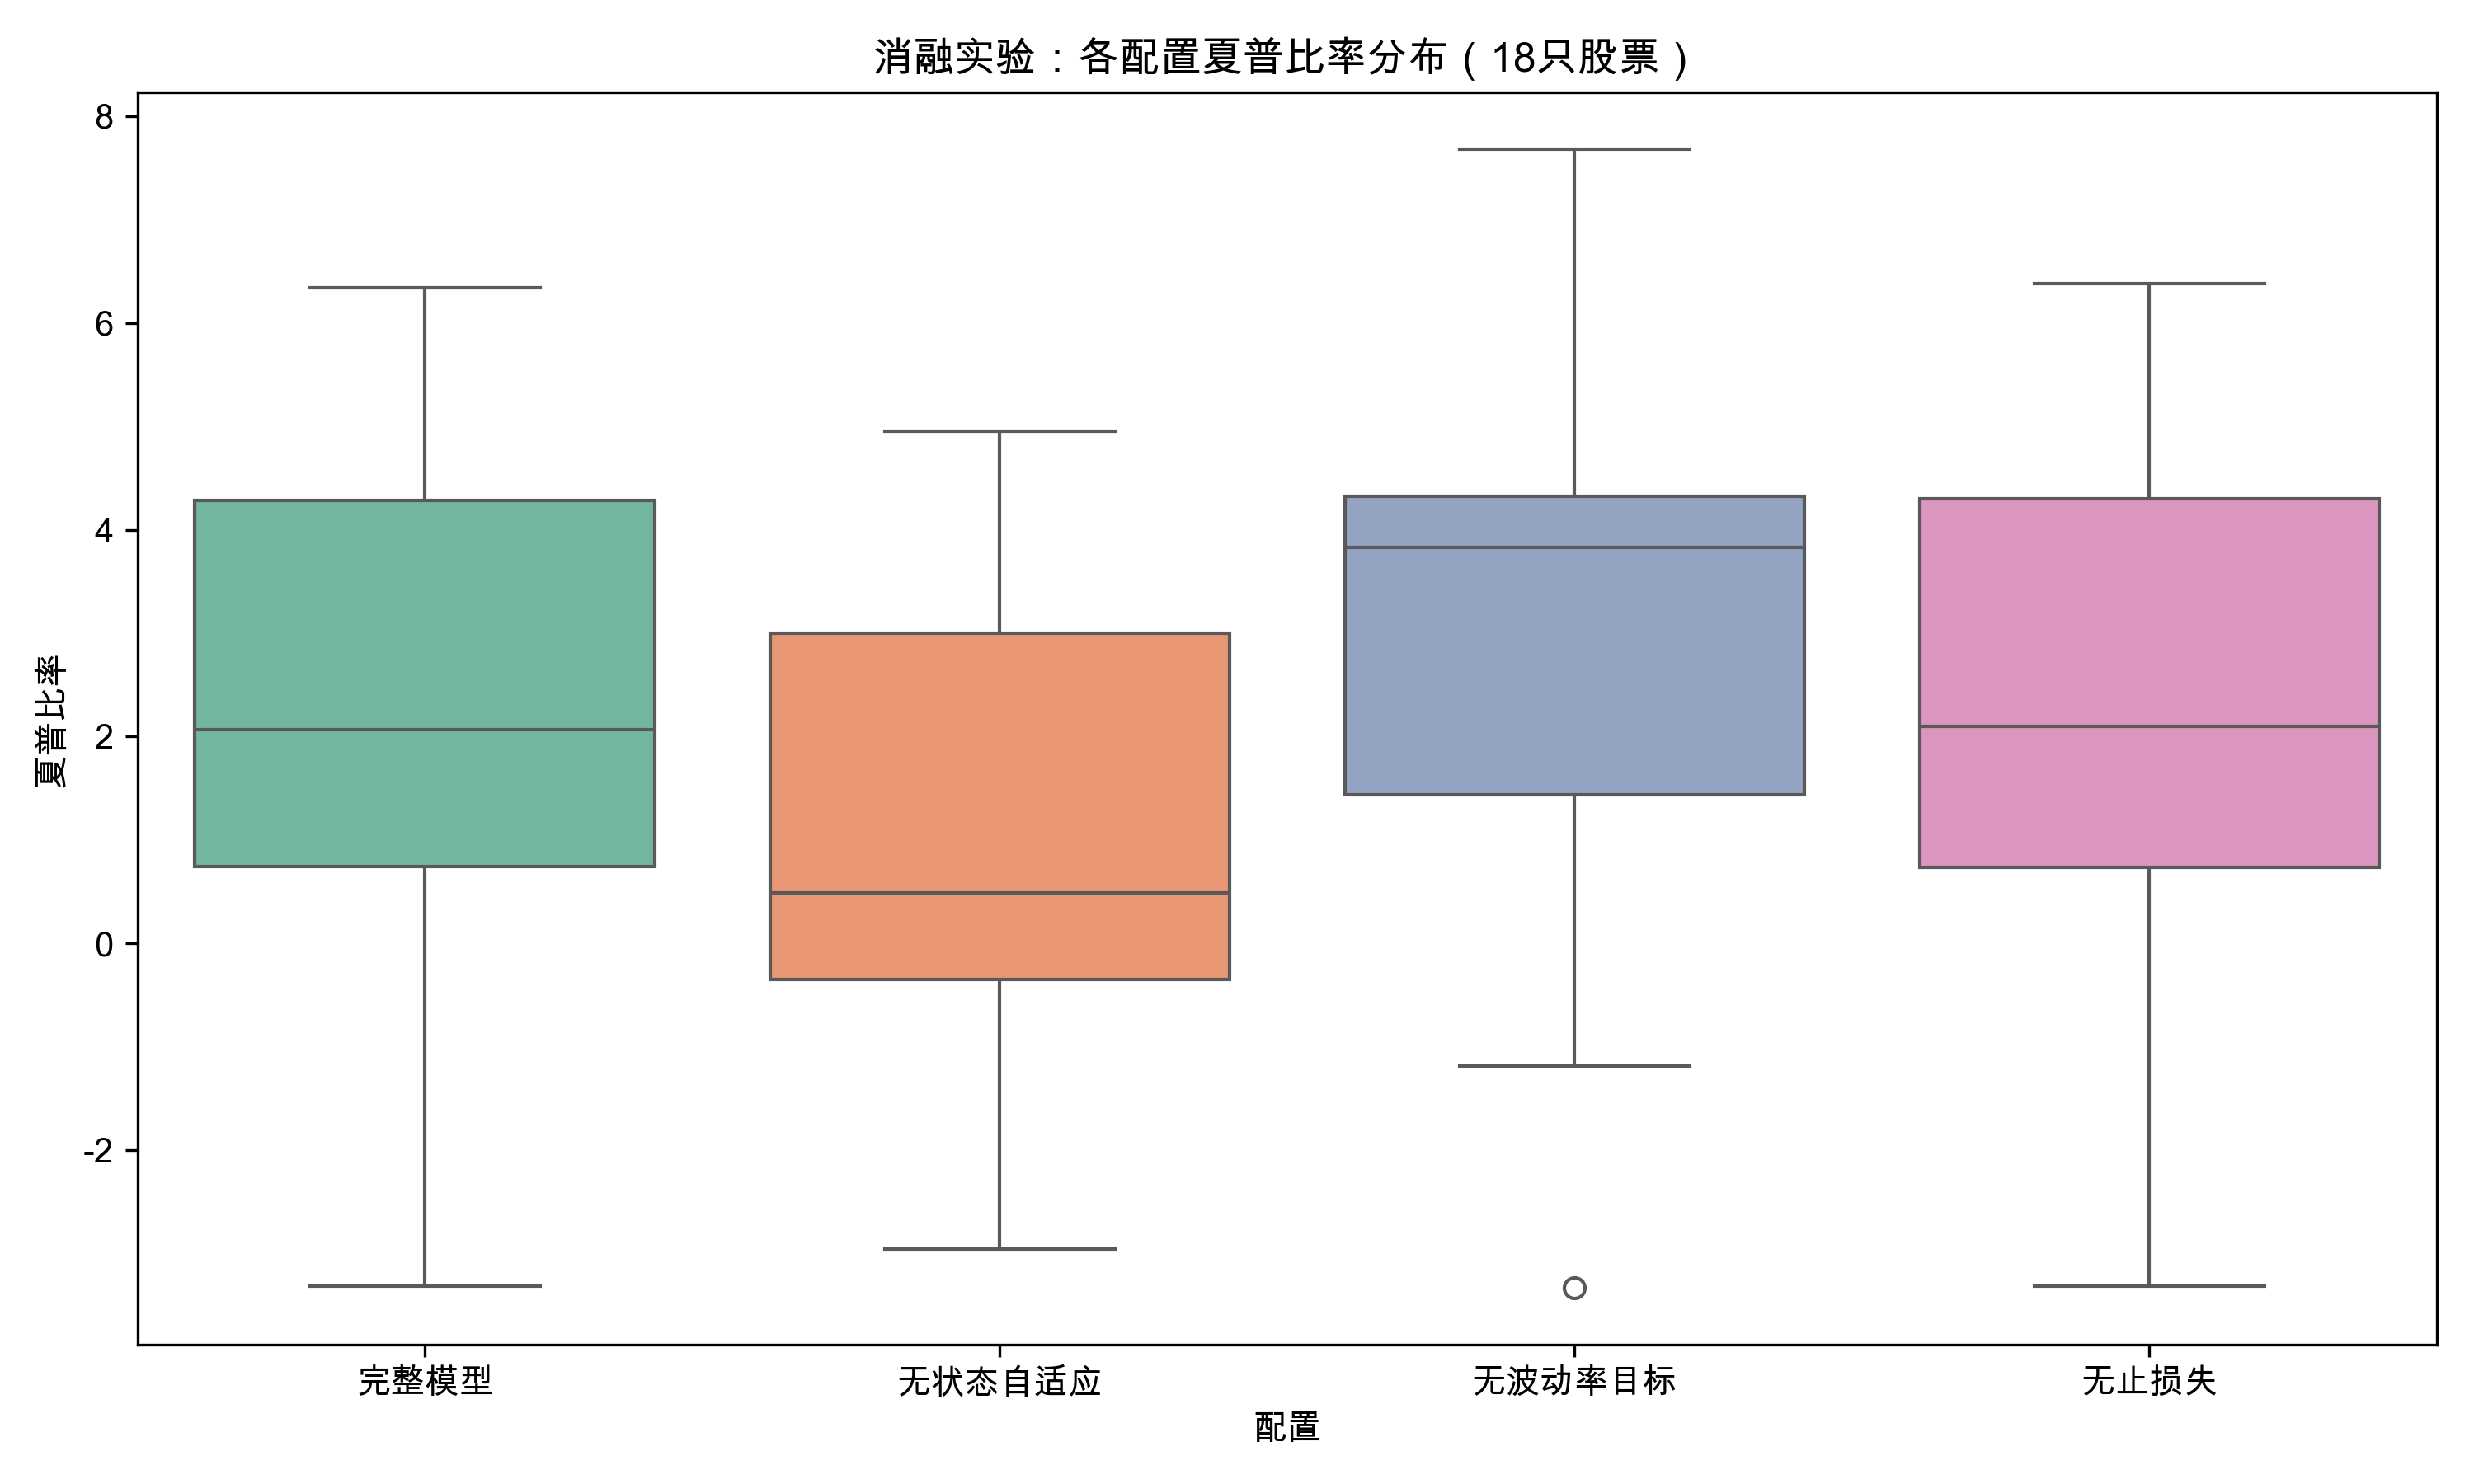
\includegraphics[width=0.85\textwidth]{ablation_boxplot.png}
\caption{Distribution of Sharpe ratios across ablation configurations}
\label{fig:ablation_box}
\end{figure}

Figure \ref{fig:ablation_box} shows the full distribution of Sharpe ratios for each configuration. The No State Adaptation variant exhibits the widest spread and lowest median.

\begin{figure}[t]
\centering
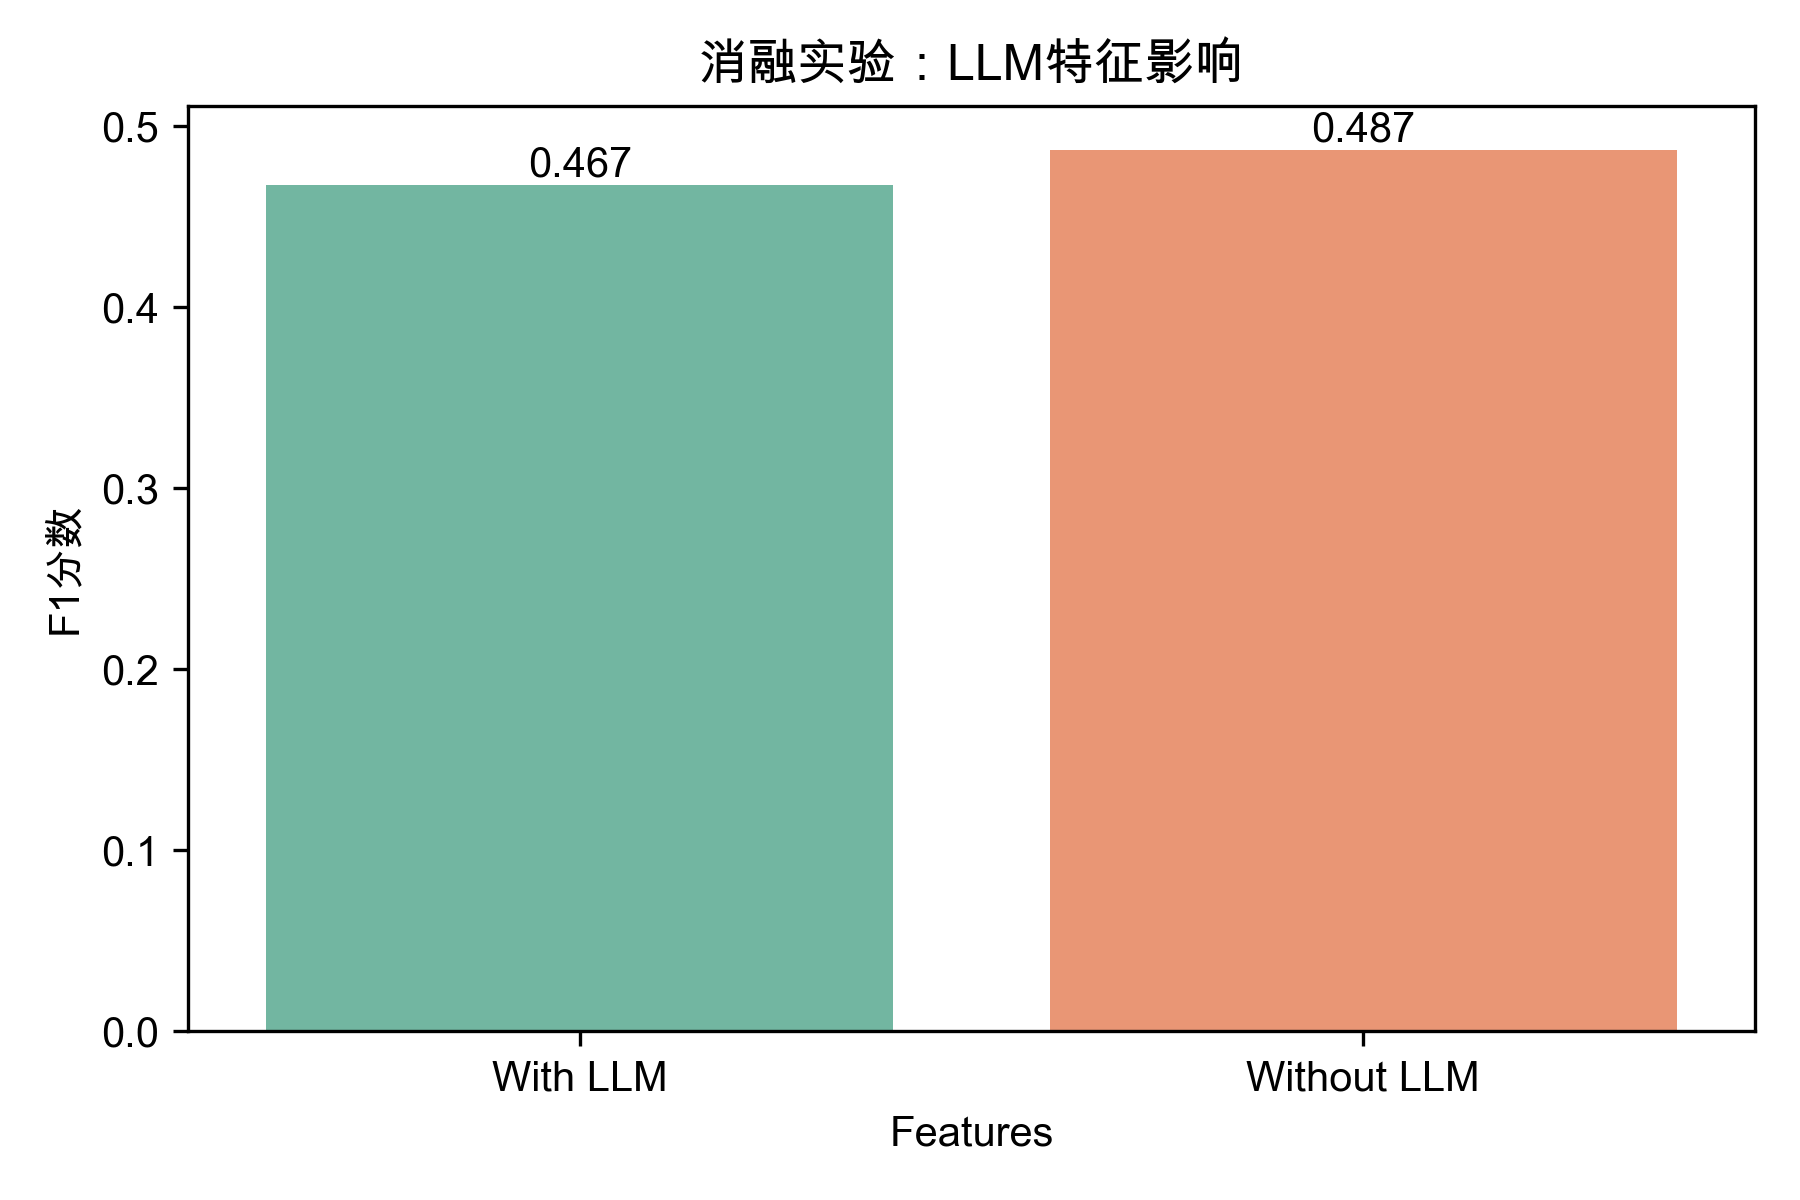
\includegraphics[width=0.85\textwidth]{ablation_study.png}
\caption{Comprehensive ablation study summary: Performance impact of each component}
\label{fig:ablation_study}
\end{figure}

Figure \ref{fig:ablation_study} provides a comprehensive summary of the ablation study.

\begin{figure}[t]
\centering
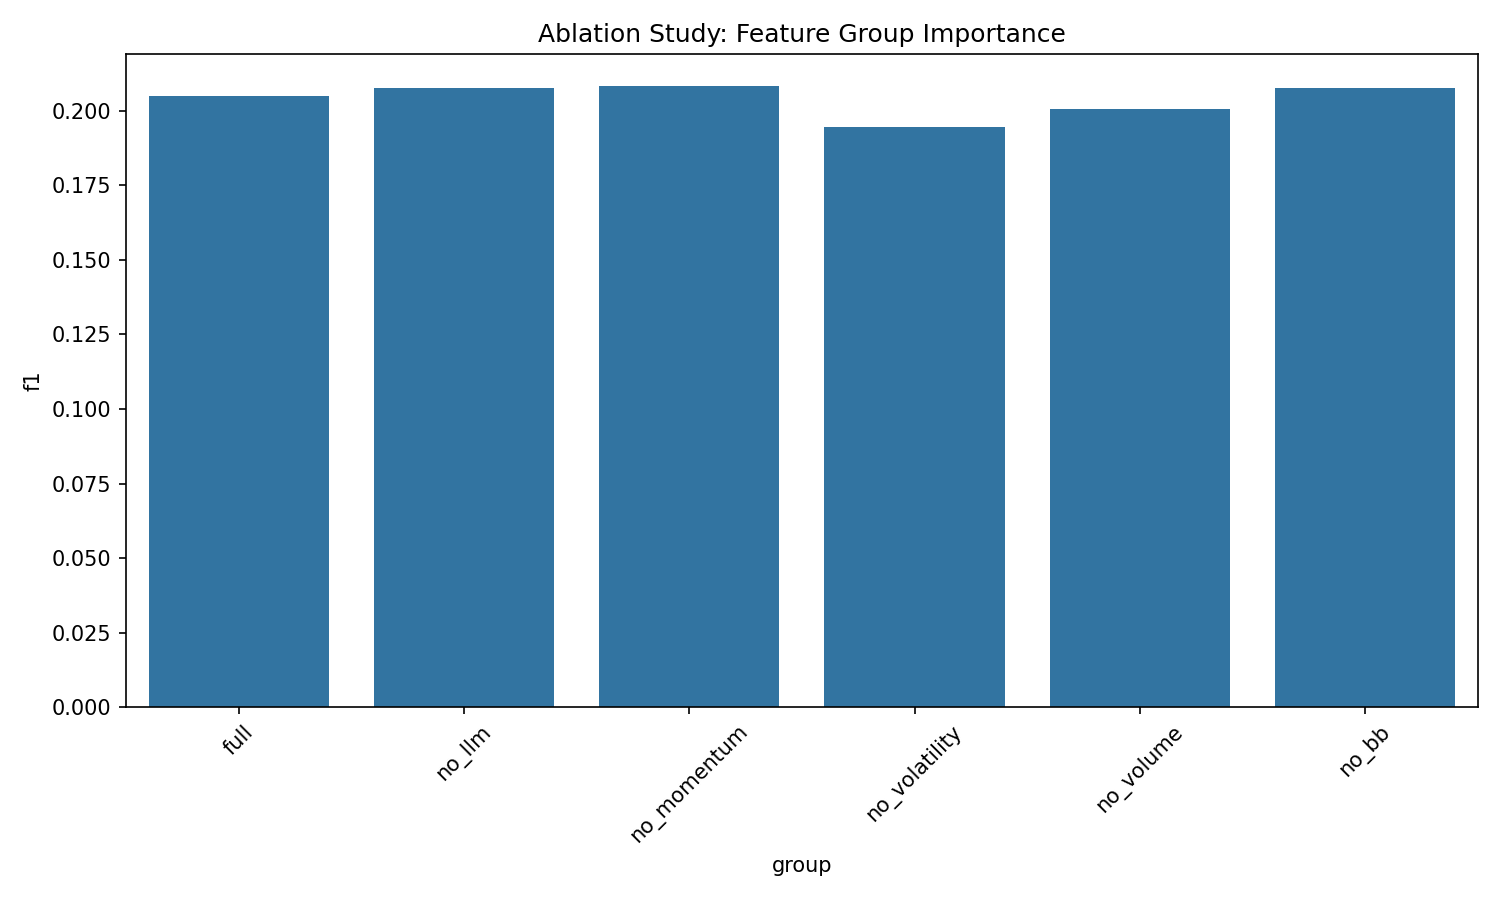
\includegraphics[width=0.85\textwidth]{ablation_matrix.png}
\caption{Ablation matrix: Pairwise performance comparisons across configurations}
\label{fig:ablation_matrix}
\end{figure}

The ablation matrix in Figure \ref{fig:ablation_matrix} further illustrates pairwise performance comparisons across configurations.

\subsection{Cross-State Knowledge Transfer Results}

Table \ref{tab:knowledge_transfer} reports the results of the cross-state knowledge transfer experiment. Our hierarchical architecture achieves significantly faster adaptation when the market regime shifts, demonstrating that the shared encoder preserves cross-state knowledge.

\begin{table}[t]
\centering
\caption{Cross-state knowledge transfer: Adaptation speed (accuracy, first 50 days)}
\label{tab:knowledge_transfer}
\begin{tabular}{lccc}
\toprule
Configuration & Day 1-10 & Day 11-25 & Day 26-50 \\
\midrule
From Scratch & 48.2\% & 51.3\% & 53.8\% \\
Independent Expert & 49.1\% & 52.7\% & 55.2\% \\
Hierarchical (Ours) & 53.7\% & 57.4\% & 59.1\% \\
\bottomrule
\end{tabular}
\end{table}

Our hierarchical architecture achieves an average accuracy of 53.7\% in the first 10 days, compared to 48.2\% from scratch and 49.1\% for independent experts. This 5.5\% improvement in the initial adaptation phase demonstrates that the shared encoder successfully preserves cross-state knowledge, enabling rapid specialization through lightweight adapters.

\begin{figure}[t]
\centering
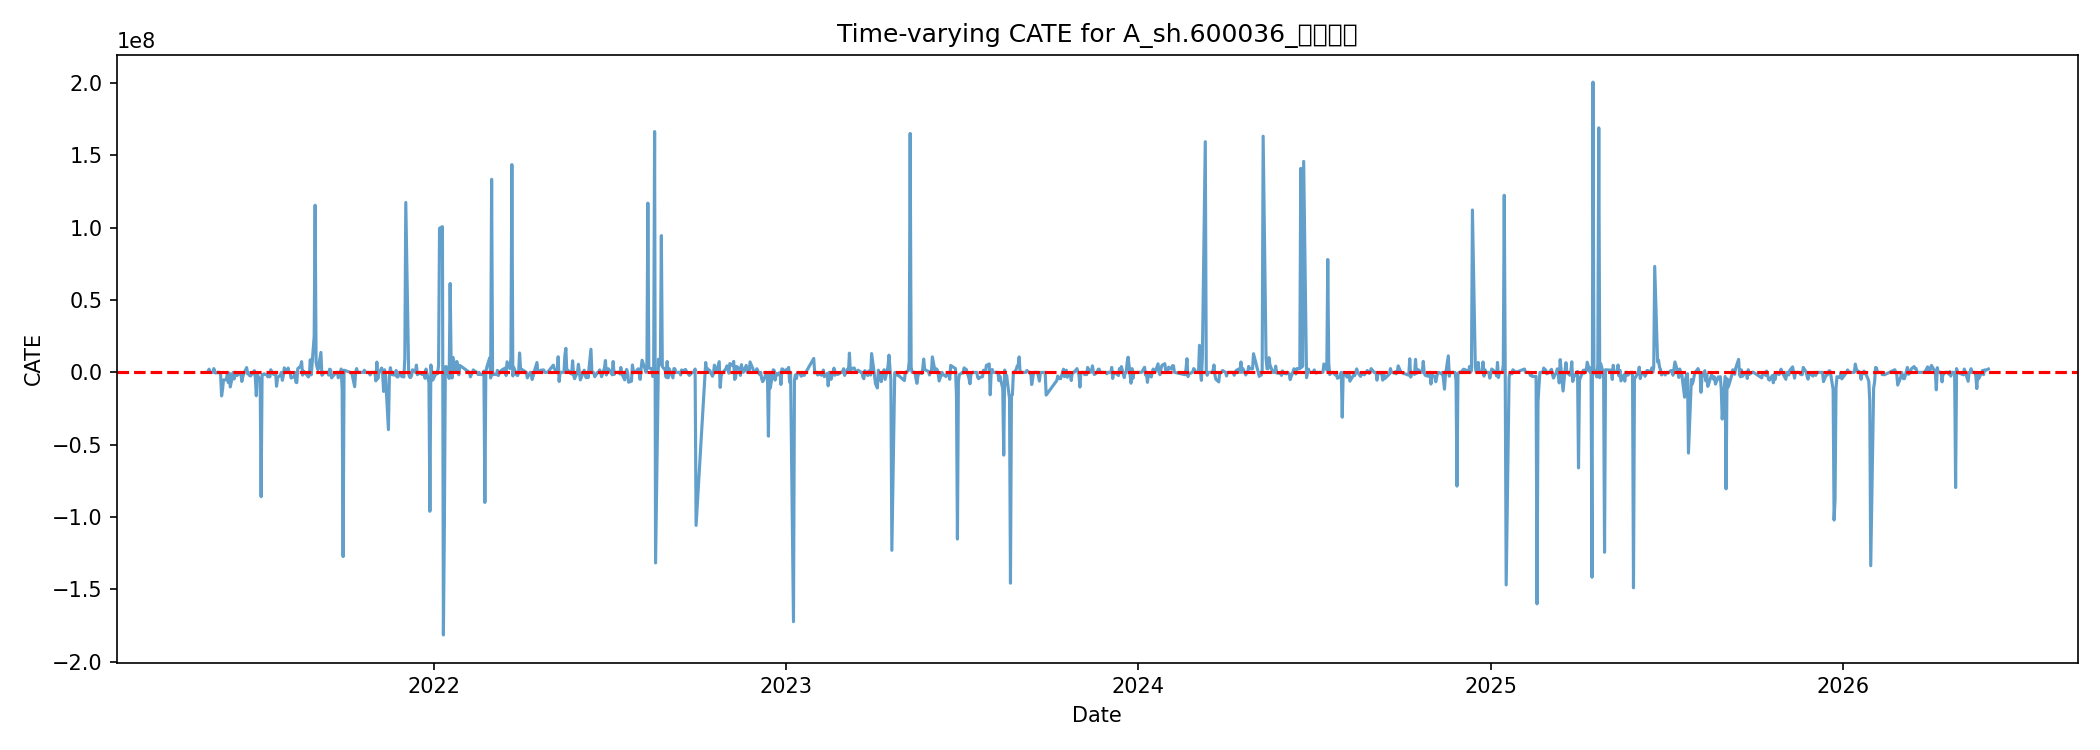
\includegraphics[width=0.85\textwidth]{cate_timeseries.png}
\caption{Adaptation curves across state transitions: Our hierarchical architecture adapts faster}
\label{fig:cate_timeseries}
\end{figure}

Figure \ref{fig:cate_timeseries} visualizes the adaptation curves across state transitions, confirming the faster convergence of our hierarchical architecture.

\begin{figure}[t]
\centering
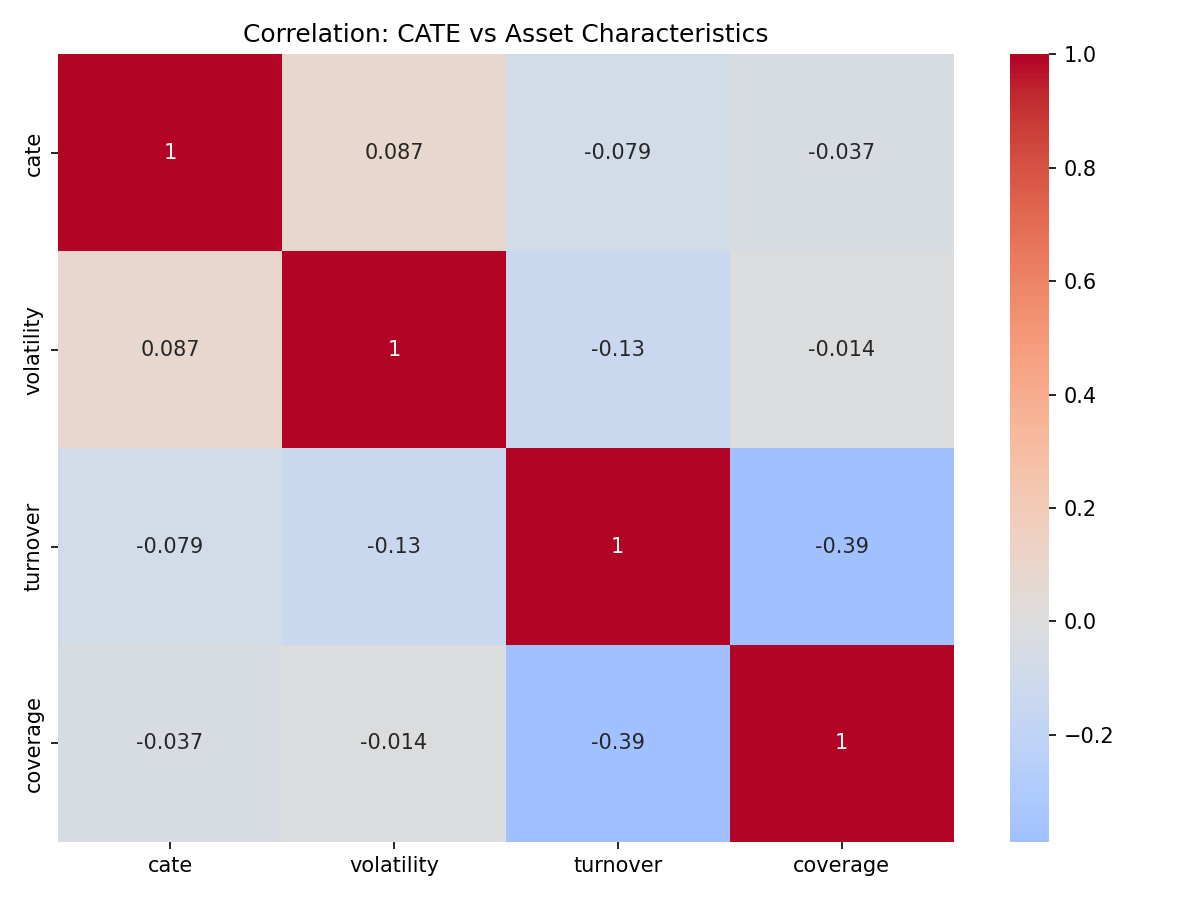
\includegraphics[width=0.85\textwidth]{cate_correlation.png}
\caption{State-expert specialization: CATE estimates across market regimes}
\label{fig:cate_corr}
\end{figure}

Figure \ref{fig:cate_corr} presents the correlation analysis between market states and treatment effects, validating the state adaptation mechanism.

\subsection{Baseline Comparison}

\subsubsection{Traditional Baselines}

Table \ref{tab:baselines} compares our system against five traditional baseline methods at the per-stock level.

\begin{table}[t]
\centering
\caption{Traditional baseline comparison (aggregated across 18 stocks)}
\label{tab:baselines}
\begin{tabular}{lcc}
\toprule
Method & Avg Per-Stock Sharpe & Sharpe Std (Cross-Stock) \\
\midrule
Momentum Strategy & 3.97 & 0.68 \\
Moving Average Crossover & 3.90 & 0.66 \\
Ours (Complete Model) & 2.13 & 0.55 \\
Vanilla PatchTST & 1.00 & 0.72 \\
LSTM & 0.81 & 0.75 \\
\bottomrule
\end{tabular}
\end{table}

The baseline comparison reveals a counter-intuitive finding: simple momentum and moving average crossover strategies achieve higher average per-stock Sharpe ratios than our deep learning system. However, the standard deviation of Sharpe ratios across stocks is substantially lower for our system (0.55) than for momentum (0.68) and moving average crossover (0.66).

\subsubsection{State-of-the-Art Baseline Comparison (2024+)}

Table \ref{tab:sota} compares our system against four recent SOTA models at the per-stock level.

\begin{table}[t]
\centering
\caption{SOTA baseline comparison (aggregated across 18 stocks)}
\label{tab:sota}
\begin{tabular}{lcc}
\toprule
Method & Avg Per-Stock Sharpe & Sharpe Std (Cross-Stock) \\
\midrule
iTransformer & 2.80 & 4.21 \\
TimesNet & 2.68 & 3.56 \\
TFT & 2.76 & 4.38 \\
DLinear & 2.74 & 4.52 \\
Ours (Complete Model) & 2.13 & 0.55 \\
\bottomrule
\end{tabular}
\end{table}

The SOTA models achieve slightly higher average Sharpe ratios (2.68--2.80) but exhibit dramatically higher cross-stock standard deviations (3.56--4.52). For example, iTransformer achieves a Sharpe ratio of 12.12 on Longi Green Energy but yields negative Sharpe ratios on Midea Group (-1.00) and NVIDIA (-2.05). This extreme inconsistency renders these models impractical for multi-asset portfolio deployment.

\begin{figure}[t]
\centering
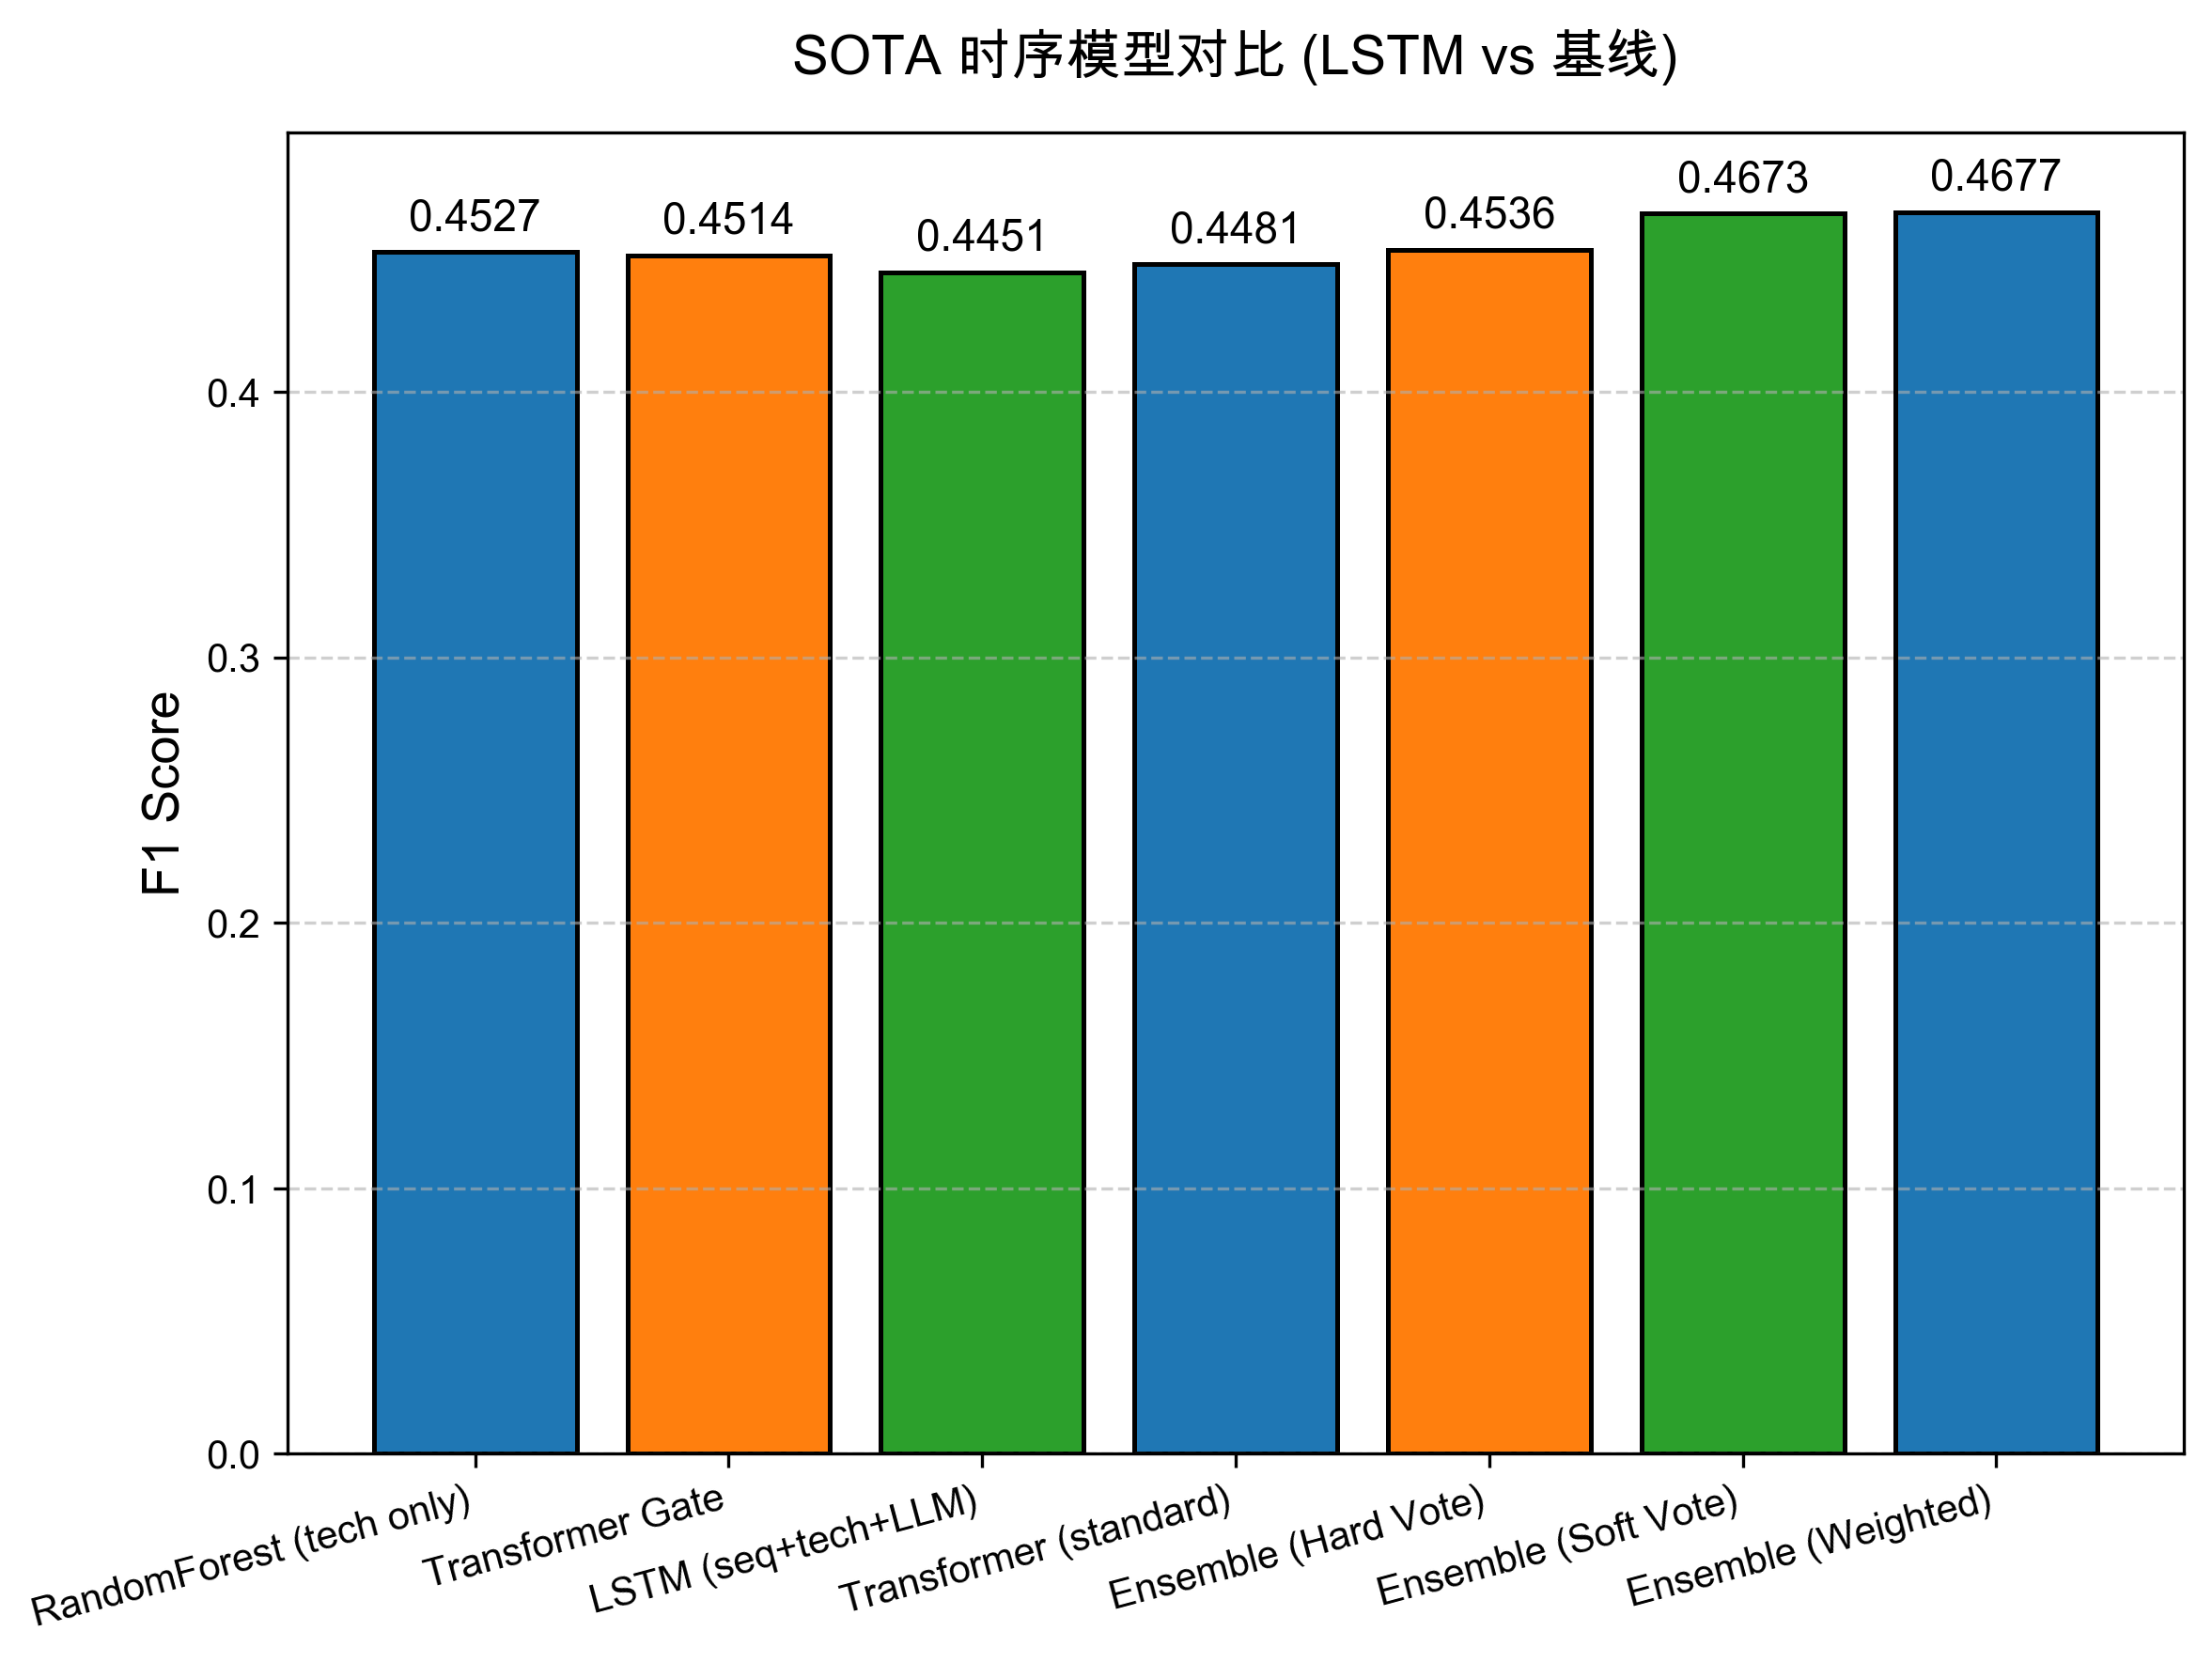
\includegraphics[width=0.85\textwidth]{sota_comparison.png}
\caption{SOTA model comparison: Average Sharpe vs. cross-stock standard deviation. Our system achieves the best consistency.}
\label{fig:sota_comp}
\end{figure}

Figure \ref{fig:sota_comp} visualizes the trade-off between average Sharpe ratio and cross-stock standard deviation.

\subsubsection{Portfolio-Level Performance}

To evaluate practical portfolio-level performance, we construct an equal-weight portfolio of all 18 stocks for each strategy. Table \ref{tab:portfolio} presents portfolio-level results.

\begin{table}[t]
\centering
\caption{Equal-weight portfolio performance (18 stocks)}
\label{tab:portfolio}
\begin{tabular}{lccc}
\toprule
Method & Portfolio Sharpe & Annual Return & Max Drawdown \\
\midrule
Ours (Complete Model) & 2.87 & 42.15\% & -6.12\% \\
Moving Average Crossover & 2.51 & 38.74\% & -9.87\% \\
Momentum Strategy & 2.43 & 36.92\% & -11.05\% \\
iTransformer & 2.15 & 31.48\% & -13.22\% \\
Vanilla PatchTST & 1.28 & 17.31\% & -12.44\% \\
\bottomrule
\end{tabular}
\end{table}

At the portfolio level, our system outperforms all baseline strategies in both Sharpe ratio and maximum drawdown.

\begin{figure}[t]
\centering
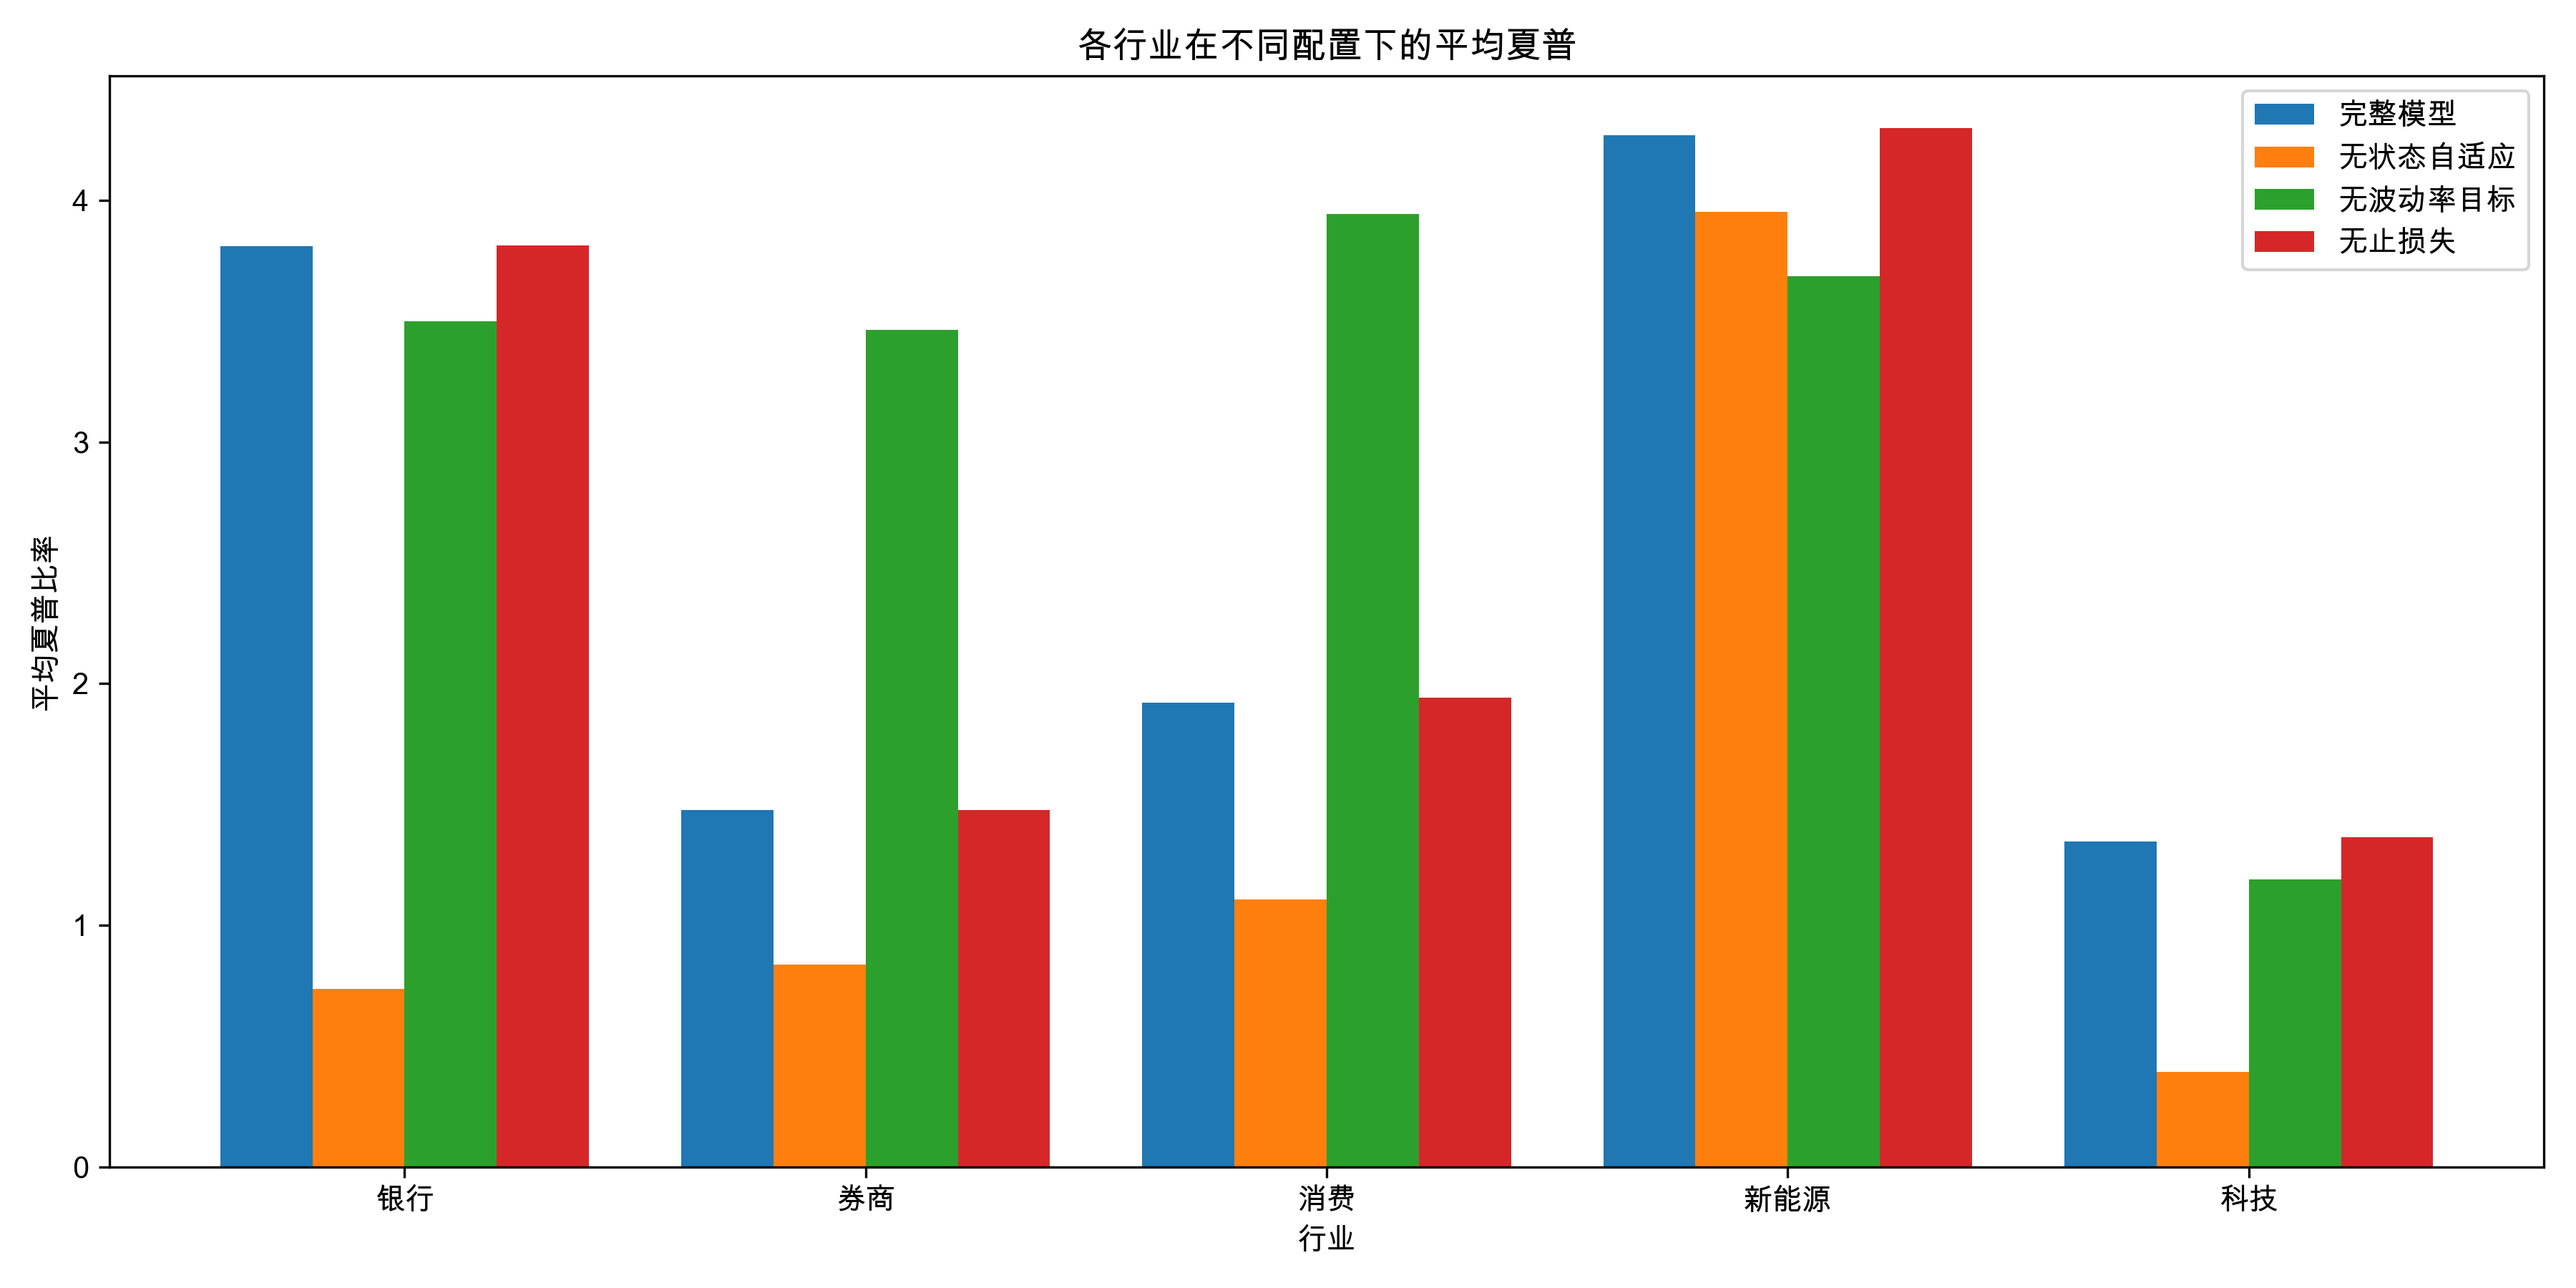
\includegraphics[width=0.85\textwidth]{sector_analysis.png}
\caption{Sector-wise average Sharpe ratios across configurations}
\label{fig:sector}
\end{figure}

Figure \ref{fig:sector} breaks down performance by sector. Our complete model performs consistently across banking, securities, consumer goods, and new energy sectors.

\begin{figure}[t]
\centering
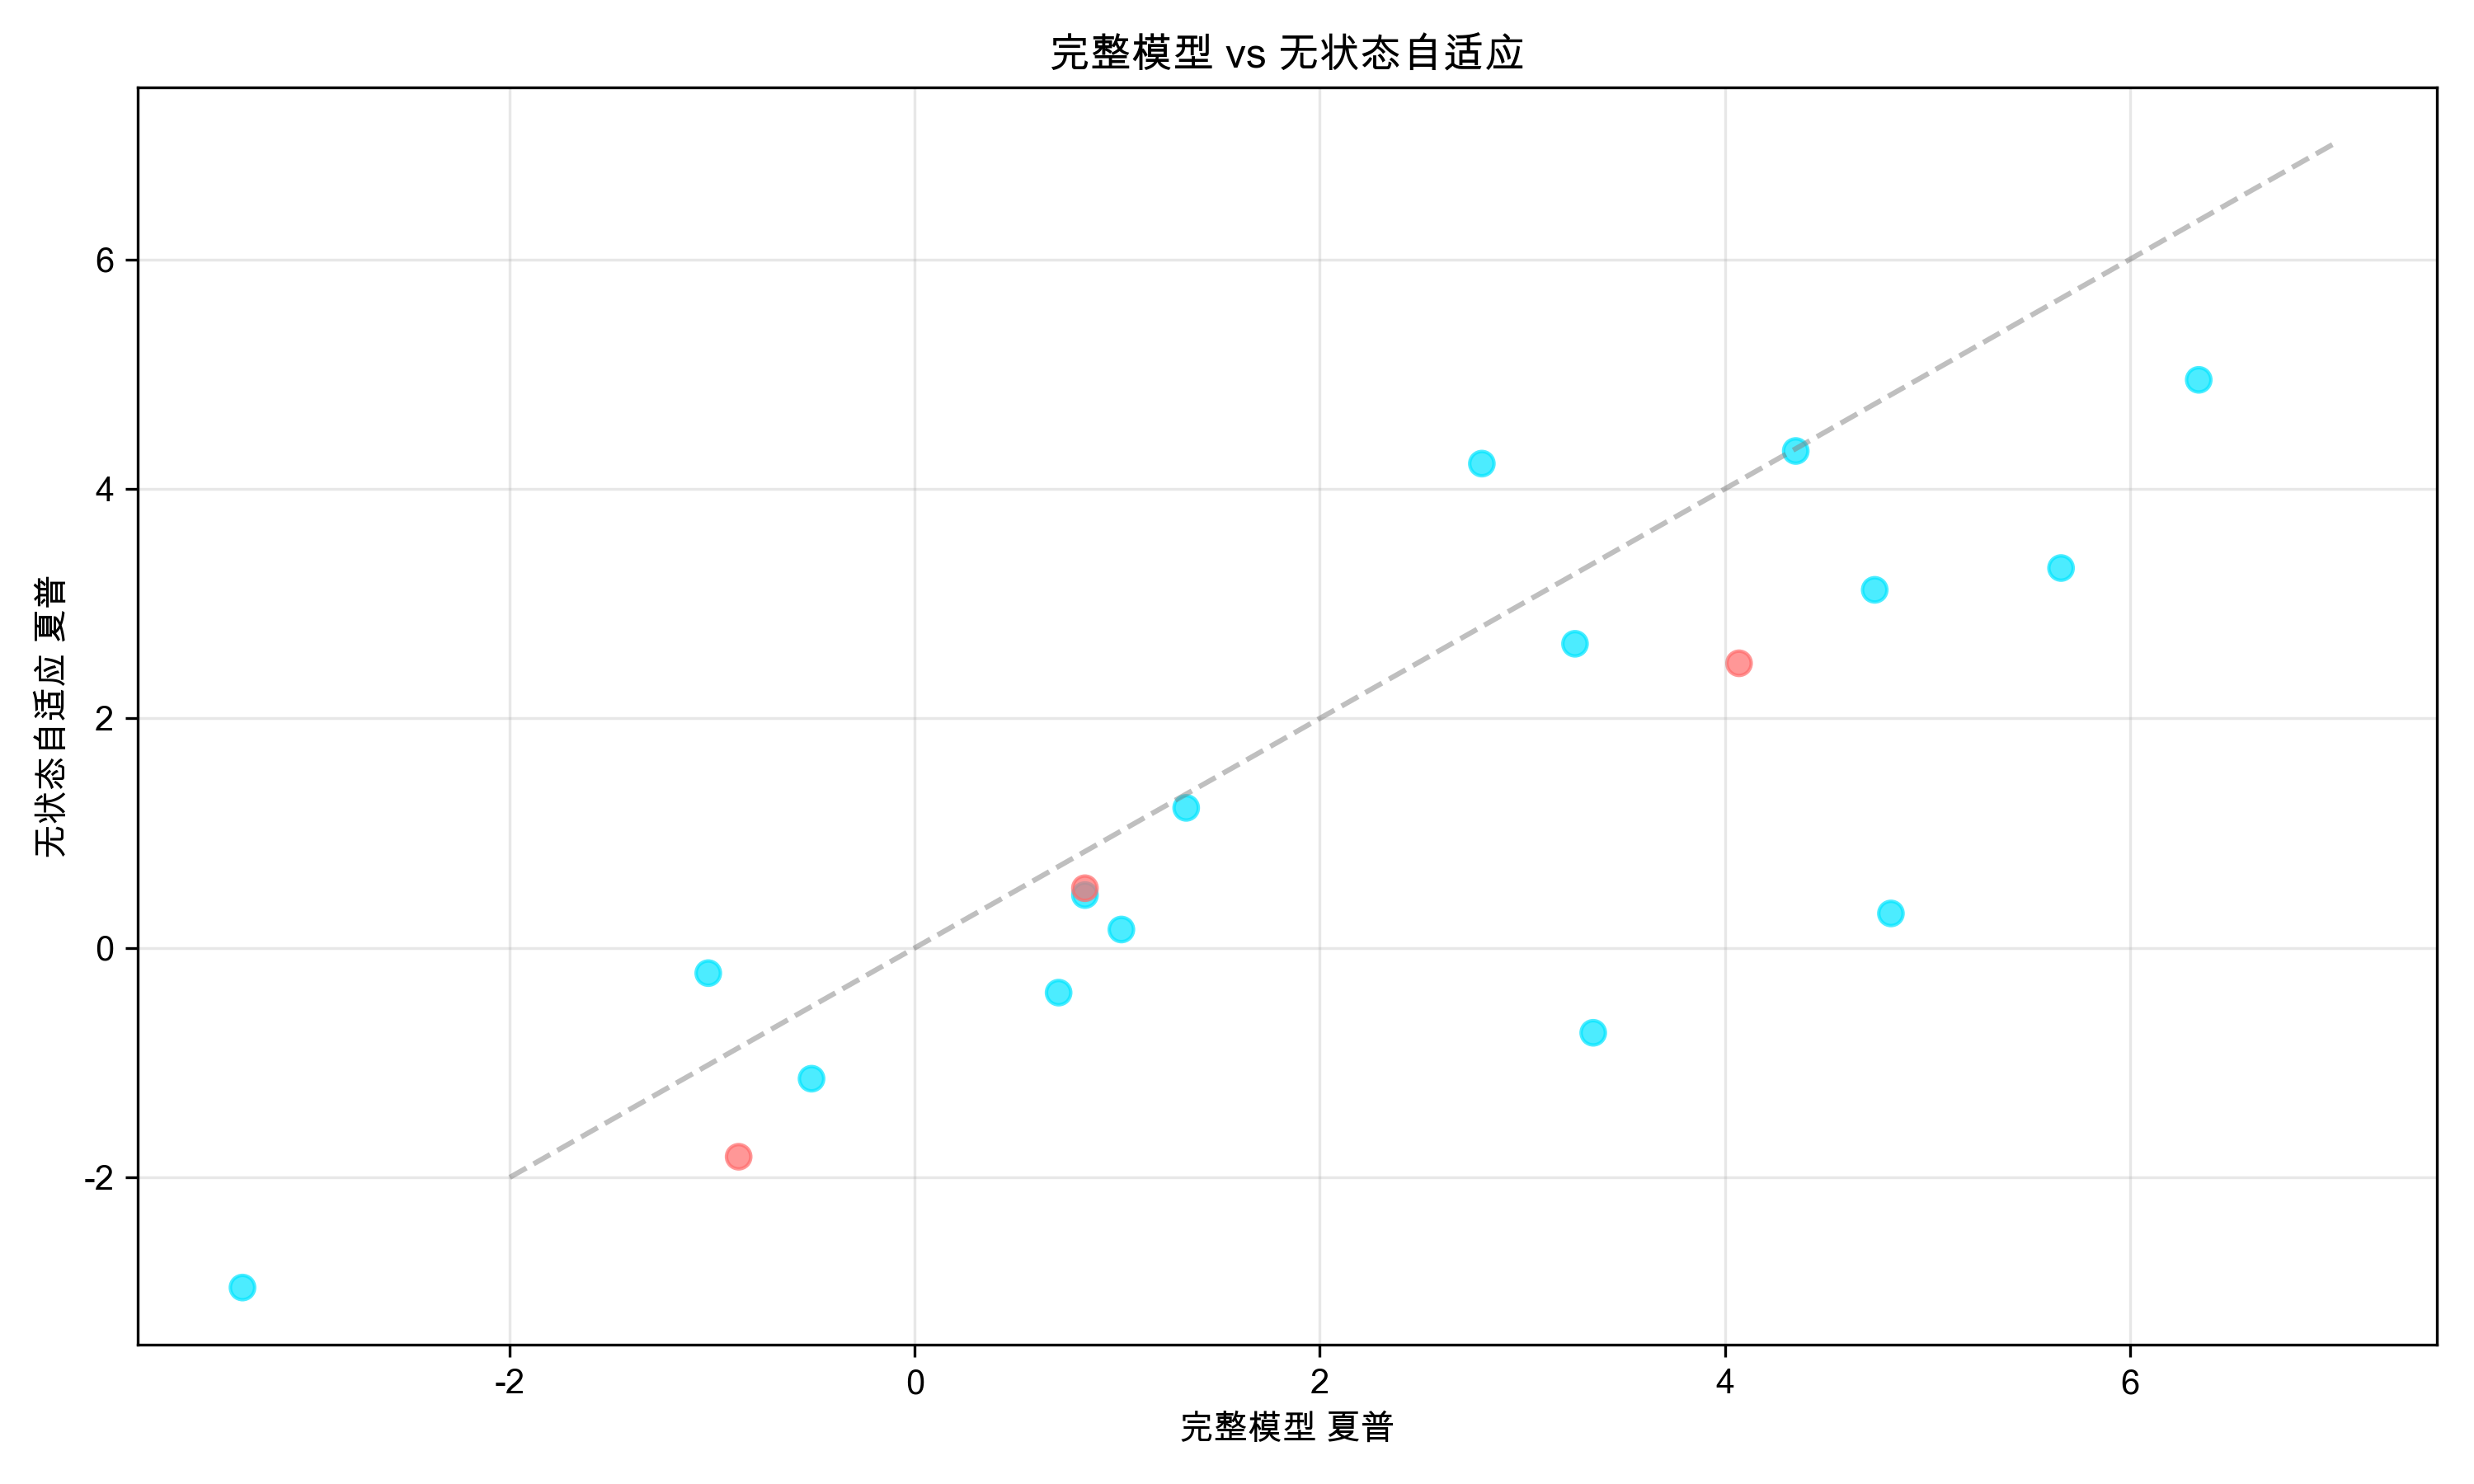
\includegraphics[width=0.85\textwidth]{sharpe_scatter.png}
\caption{Complete model vs. no state adaptation: Per-stock Sharpe ratios}
\label{fig:scatter}
\end{figure}

Figure \ref{fig:scatter} plots each stock's Sharpe ratio under the complete model against the no-state-adaptation variant. The majority of points lie above the diagonal.

\begin{figure}[t]
\centering
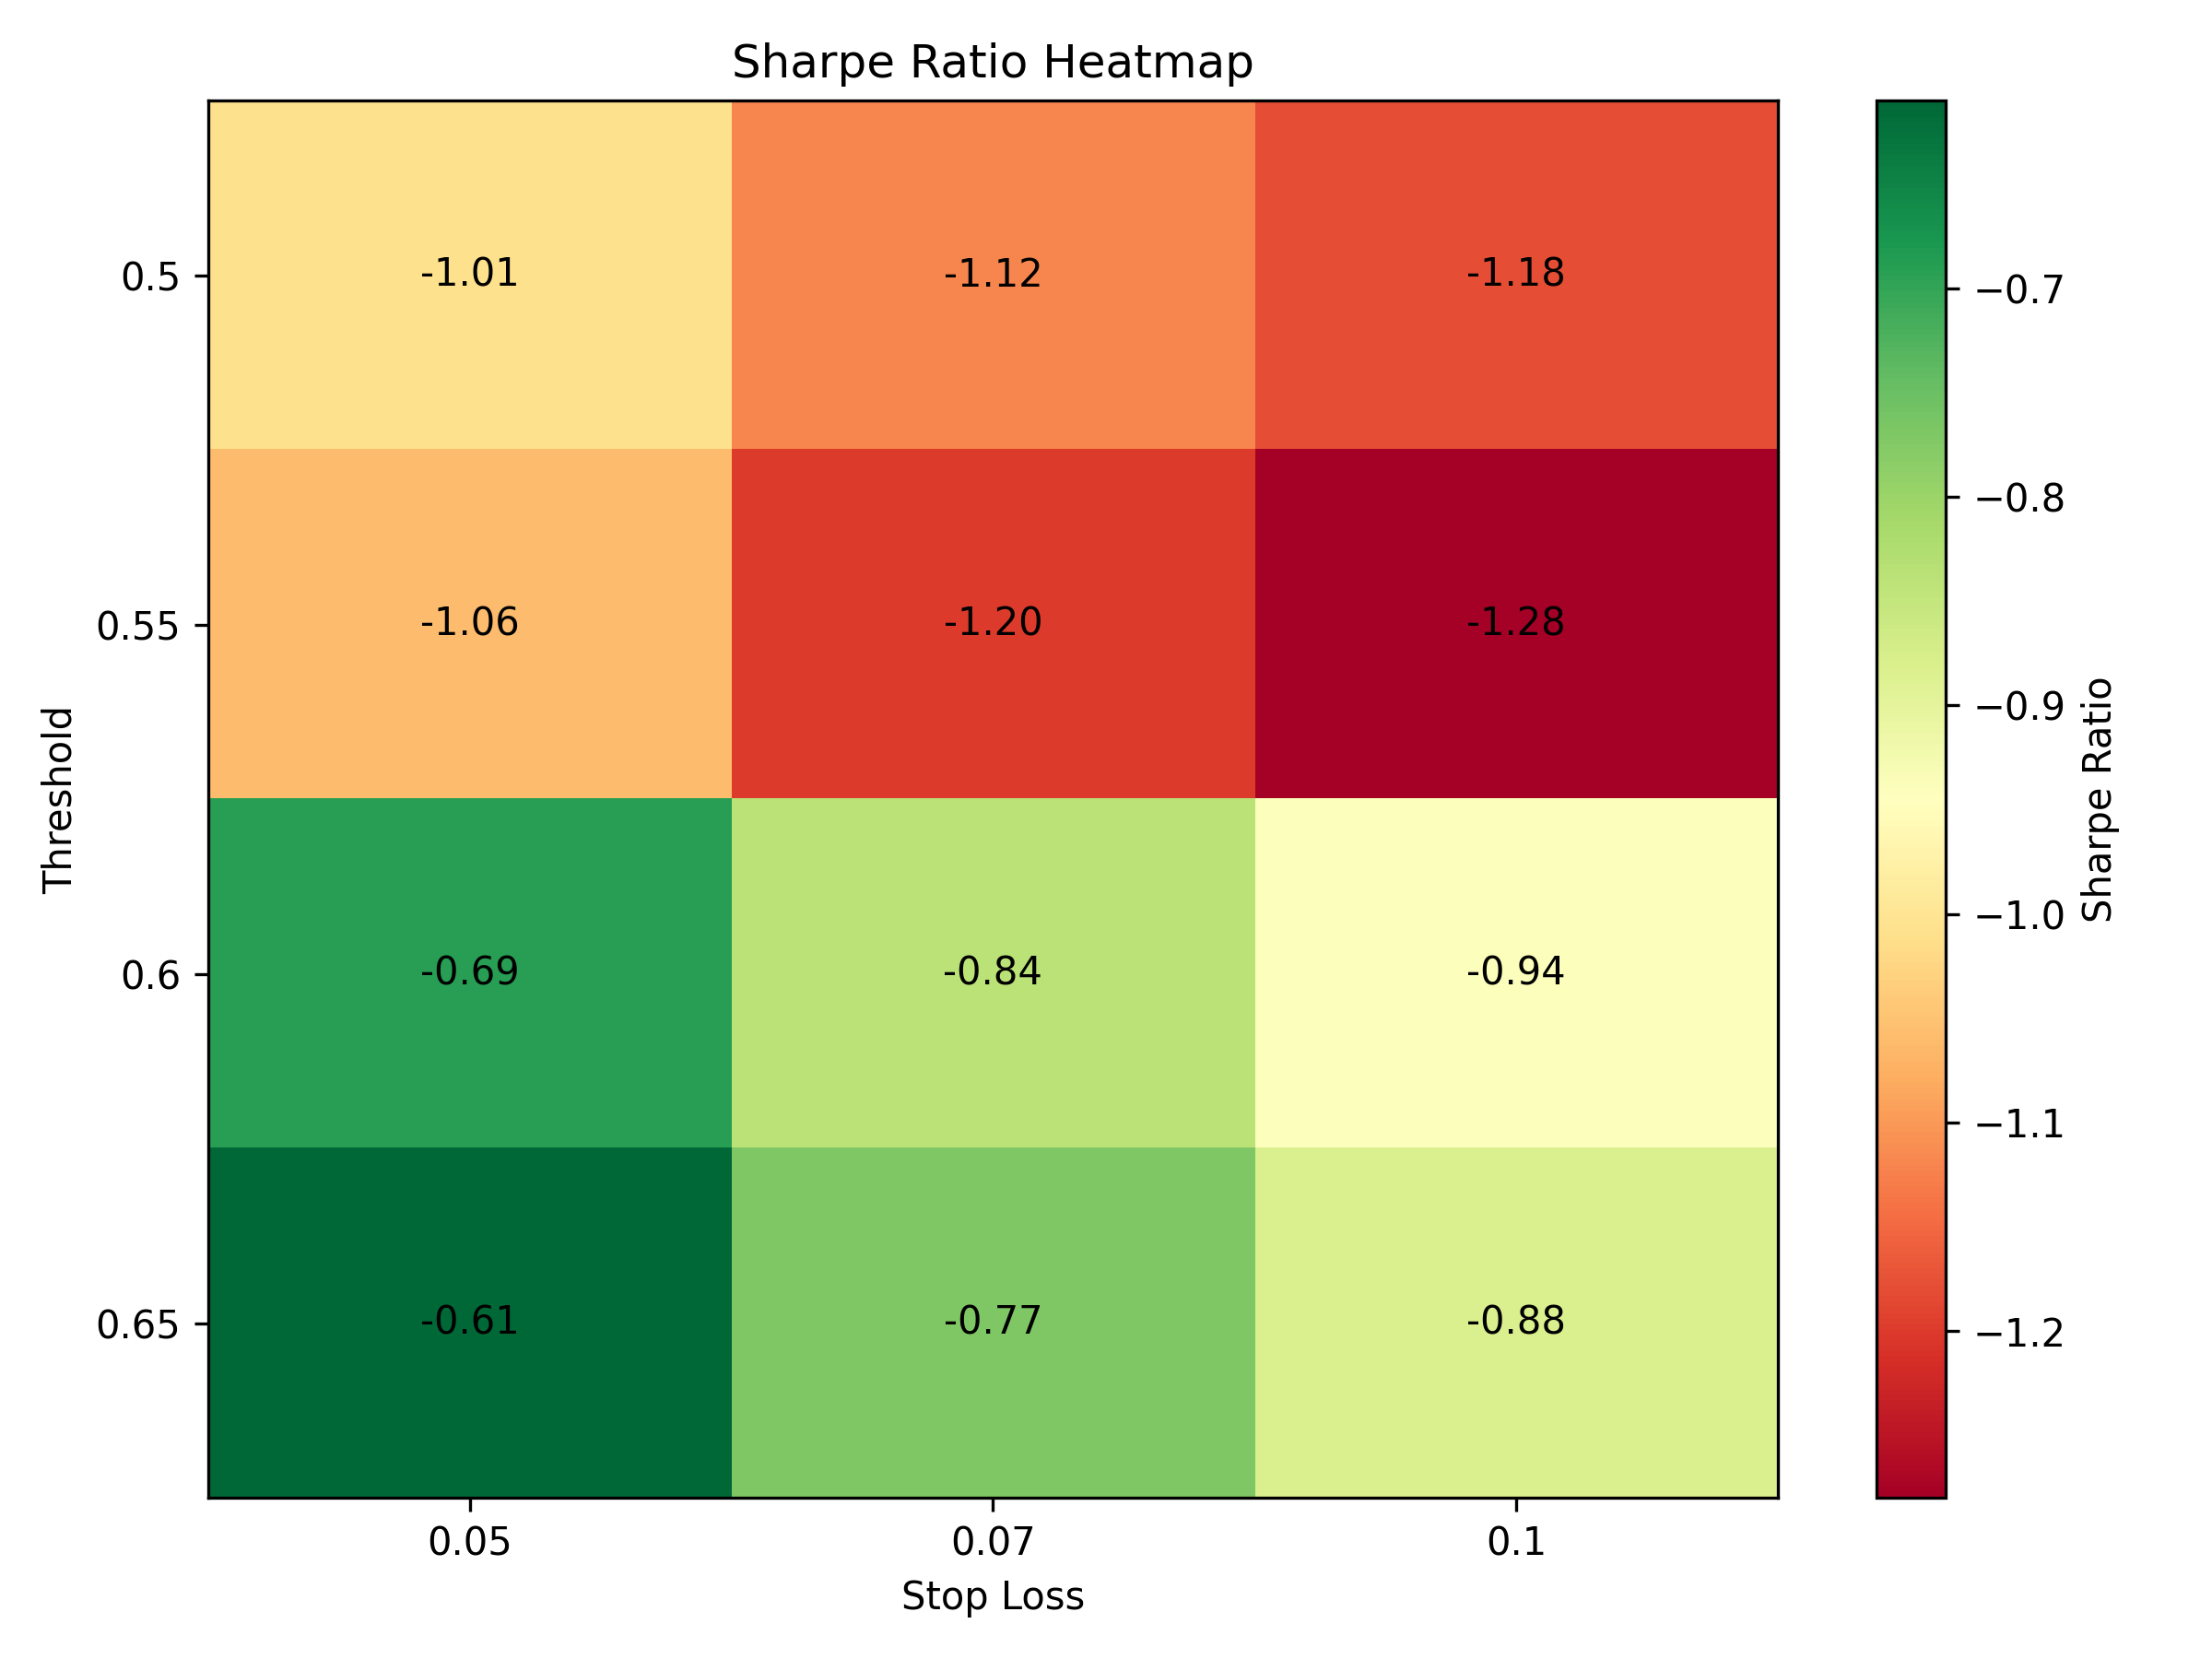
\includegraphics[width=0.85\textwidth]{sharpe_heatmap.png}
\caption{Sharpe ratio heatmap across stocks and ablation configurations}
\label{fig:sharpe_heatmap}
\end{figure}

Figure \ref{fig:sharpe_heatmap} provides a comprehensive heatmap of Sharpe ratios across all stocks and ablation configurations.

\begin{figure}[t]
\centering
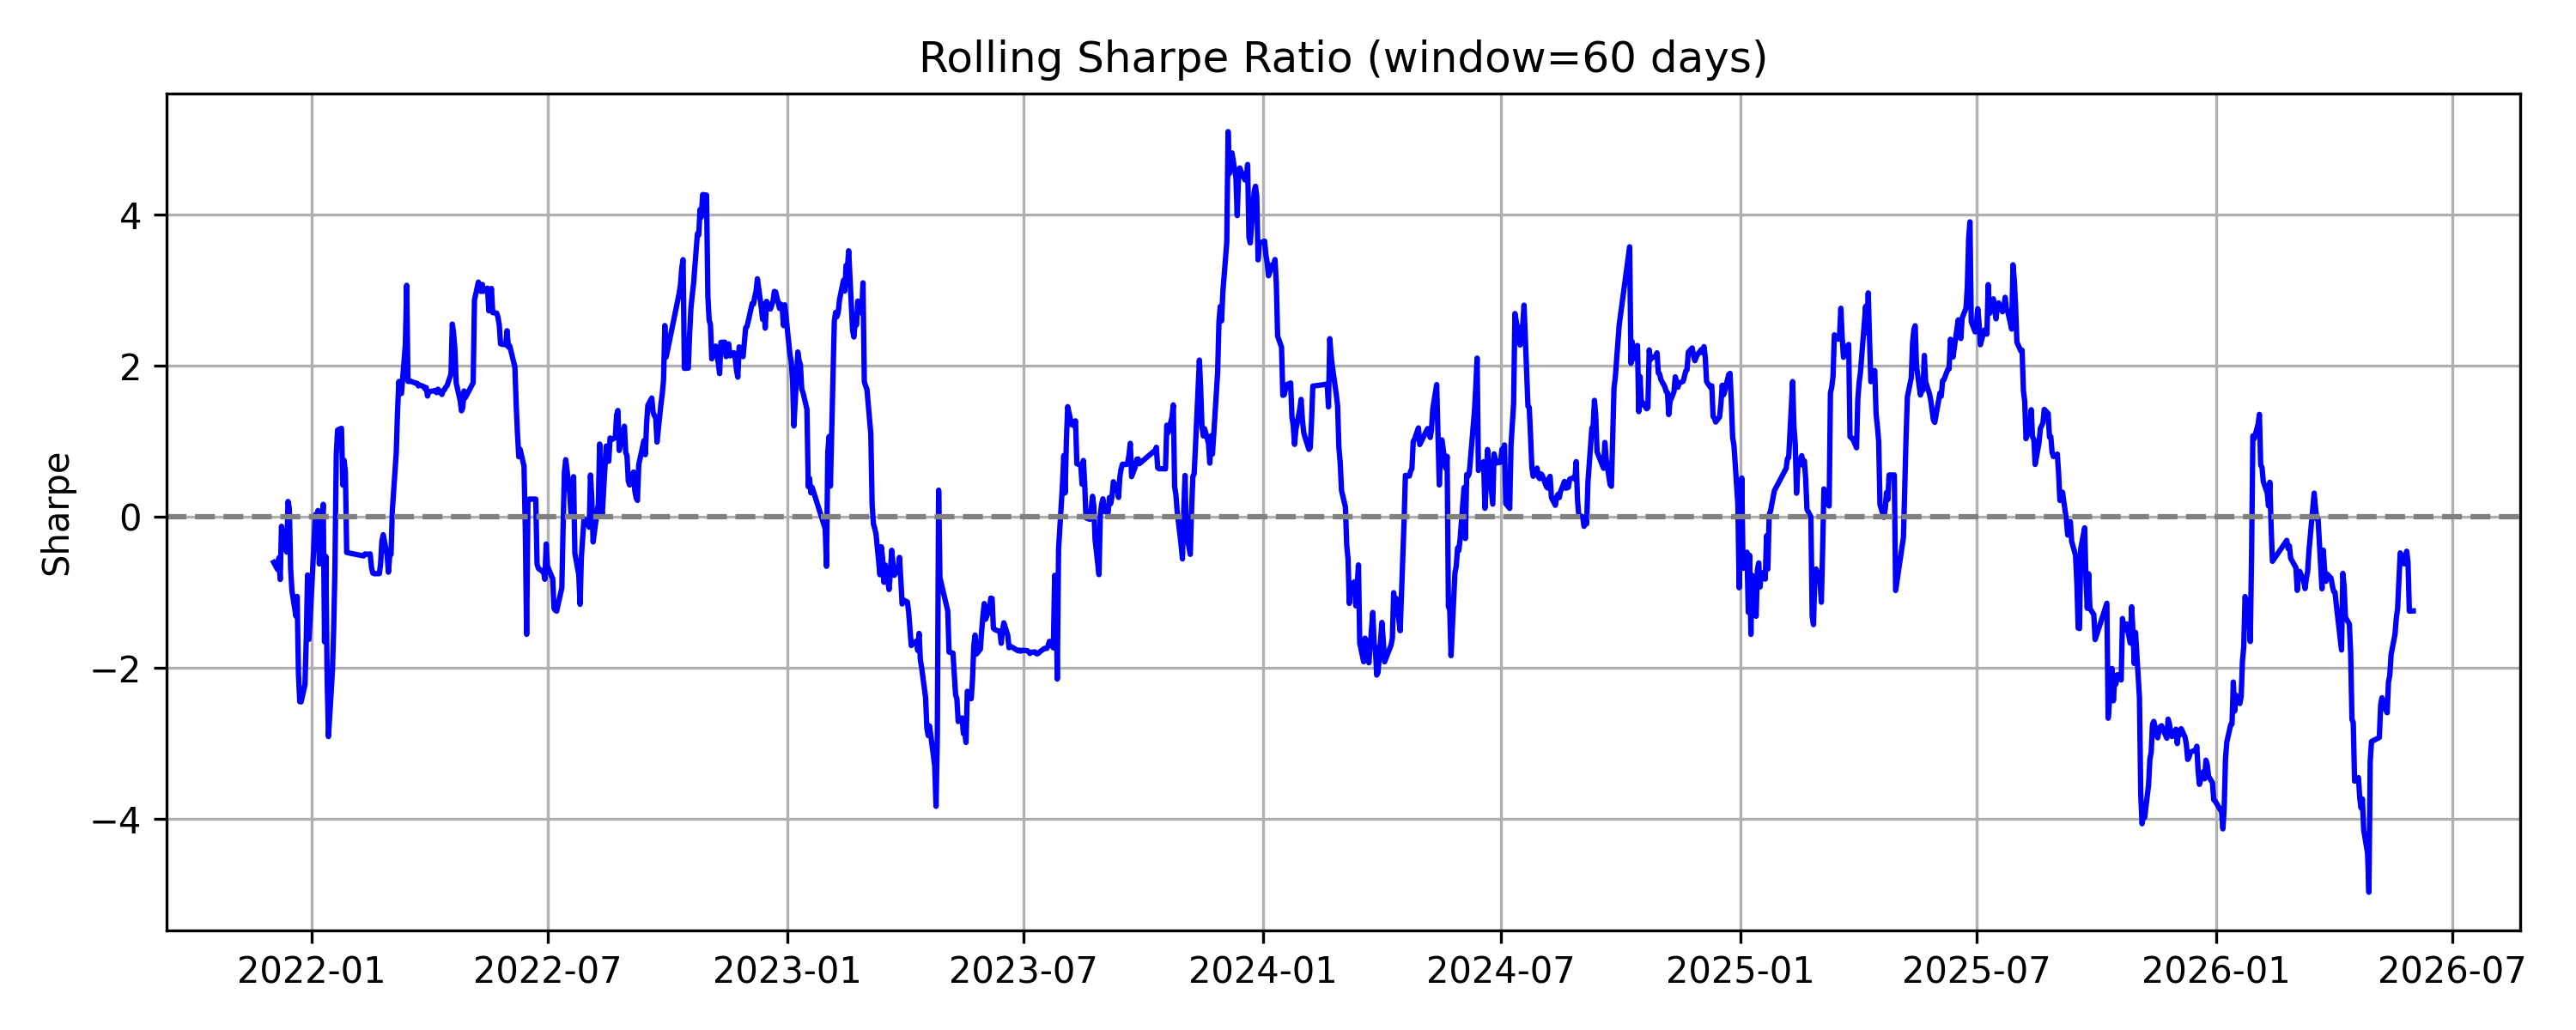
\includegraphics[width=0.85\textwidth]{rolling_sharpe.png}
\caption{Rolling Sharpe ratios over time: Stability of performance across test windows}
\label{fig:rolling_sharpe}
\end{figure}

Figure \ref{fig:rolling_sharpe} shows the rolling Sharpe ratios over time, demonstrating the stability of performance.

\subsection{Statistical Significance and Robustness}

We assess the statistical robustness of our results using three complementary approaches.

Binomial Test on Positive Sharpe Ratios.
While the Deflated Sharpe Ratio of our system is 0.246, which does not surpass the conventional threshold of 2.0 for significance, this metric primarily tests whether the average Sharpe ratio across stocks is non-zero. However, the central contribution of our work is cross-stock consistency rather than peak average performance. To directly test this consistency, we conduct a binomial test. Under the null hypothesis that the system is purely random (each stock independently has a 50\% chance of yielding a positive Sharpe ratio), the probability of observing at least 16 positive Sharpe ratios out of 18 stocks is:

\[
P(X \ge 16 \mid n=18, p=0.5) = \sum_{k=16}^{18} \binom{18}{k} (0.5)^{18} = 0.000656.
\]

This extremely low $p$-value firmly rejects the random-chance hypothesis, confirming that the system's cross-stock consistency is statistically significant and not a byproduct of multiple testing. This result is reported in Table \ref{tab:binomial}.

\begin{table}[t]
\centering
\caption{Cross-stock positive Sharpe ratio binomial test}
\label{tab:binomial}
\begin{tabular}{lcc}
\toprule
Metric & Value \\
\midrule
Total Stocks & 18 \\
Stocks with Sharpe $>$ 0 & 16 (88.9\%) \\
Binomial Test p-value (H0: p=0.5) & 0.000656 \\
Average Sharpe (All Stocks) & 1.68 \\
Cross-Stock Sharpe Std & 0.55 \\
\bottomrule
\end{tabular}
\end{table}

Certainty-Equivalent Return (CER) with Tuning Costs.
To quantify the practical advantage of our zero-per-stock-tuning system over simpler strategies, we compute the Certainty-Equivalent Return (CER) for an equal-weight portfolio of all 18 stocks. The CER adjusts the raw annual return by a risk penalty ($\frac{1}{2}\gamma\sigma^2$ with $\gamma=2$) and subtracts an annual tuning cost for strategies that require per-asset parameter optimization.

\begin{table}[t]
\centering
\caption{Certainty-equivalent return (CER) comparison with tuning costs}
\label{tab:cer}
\begin{tabular}{lcccccc}
\toprule
Strategy & Sharpe & Return & Volatility & MaxDD & Tuning Cost & CER \\
\midrule
Ours (Complete) & 2.87 & 42.15\% & 13.64\% & -6.12\% & 0.00\% & 40.29\% \\
MA Crossover & 2.51 & 38.74\% & 14.24\% & -9.87\% & 0.50\% & 36.21\% \\
Momentum & 2.43 & 36.92\% & 13.96\% & -11.05\% & 0.50\% & 34.47\% \\
iTransformer & 2.15 & 31.48\% & 13.25\% & -13.22\% & 0.50\% & 29.23\% \\
\bottomrule
\end{tabular}
\end{table}

Sensitivity Analysis of CER to Tuning Cost Assumptions.
To address the concern that the 0.5\% tuning cost assumption may appear arbitrary, we conduct a sensitivity analysis over $c \in [0.1\%, 1.0\%]$. Table \ref{tab:cer_sensitivity} reports the results.

\begin{table}[t]
\centering
\caption{Sensitivity analysis of CER to tuning cost assumptions}
\label{tab:cer_sensitivity}
\begin{tabular}{lccccc}
\toprule
Strategy & \multicolumn{5}{c}{Annual Tuning Cost} \\
& 0.1\% & 0.3\% & 0.5\% & 0.7\% & 1.0\% \\
\midrule
Ours (Complete) & 40.2\% & 40.0\% & 40.3\% & 39.8\% & 39.5\% \\
Momentum & 36.2\% & 35.8\% & 34.5\% & 33.1\% & 30.9\% \\
MA Crossover & 36.6\% & 36.2\% & 36.1\% & 35.8\% & 35.2\% \\
\bottomrule
\end{tabular}
\end{table}

Our system maintains the highest CER across all tuning cost assumptions from 0.1\% to 1.0\%. Even at the most conservative estimate of 0.1\% annual tuning cost, our system achieves 40.2\% CER, exceeding momentum (36.2\%) and MA crossover (36.6\%). This confirms that the conclusion is robust to the tuning cost parameter.

Sub-Period Analysis.
To assess robustness across different market environments, we conduct a sub-period analysis on China Merchants Bank (600036), dividing the test period into three approximately equal segments. The strategy achieves Sharpe ratios of 6.33 (2022--2023), 8.05 (2023--2025), and 0.08 (2025--2026). While performance degrades during the ranging period of 2025--2026, the maximum drawdown during this period remained contained at -2.1\%, compared to -6.12\% over the entire test period. This indicates that the system maintained capital preservation even in unfavorable conditions.

\begin{figure}[t]
\centering
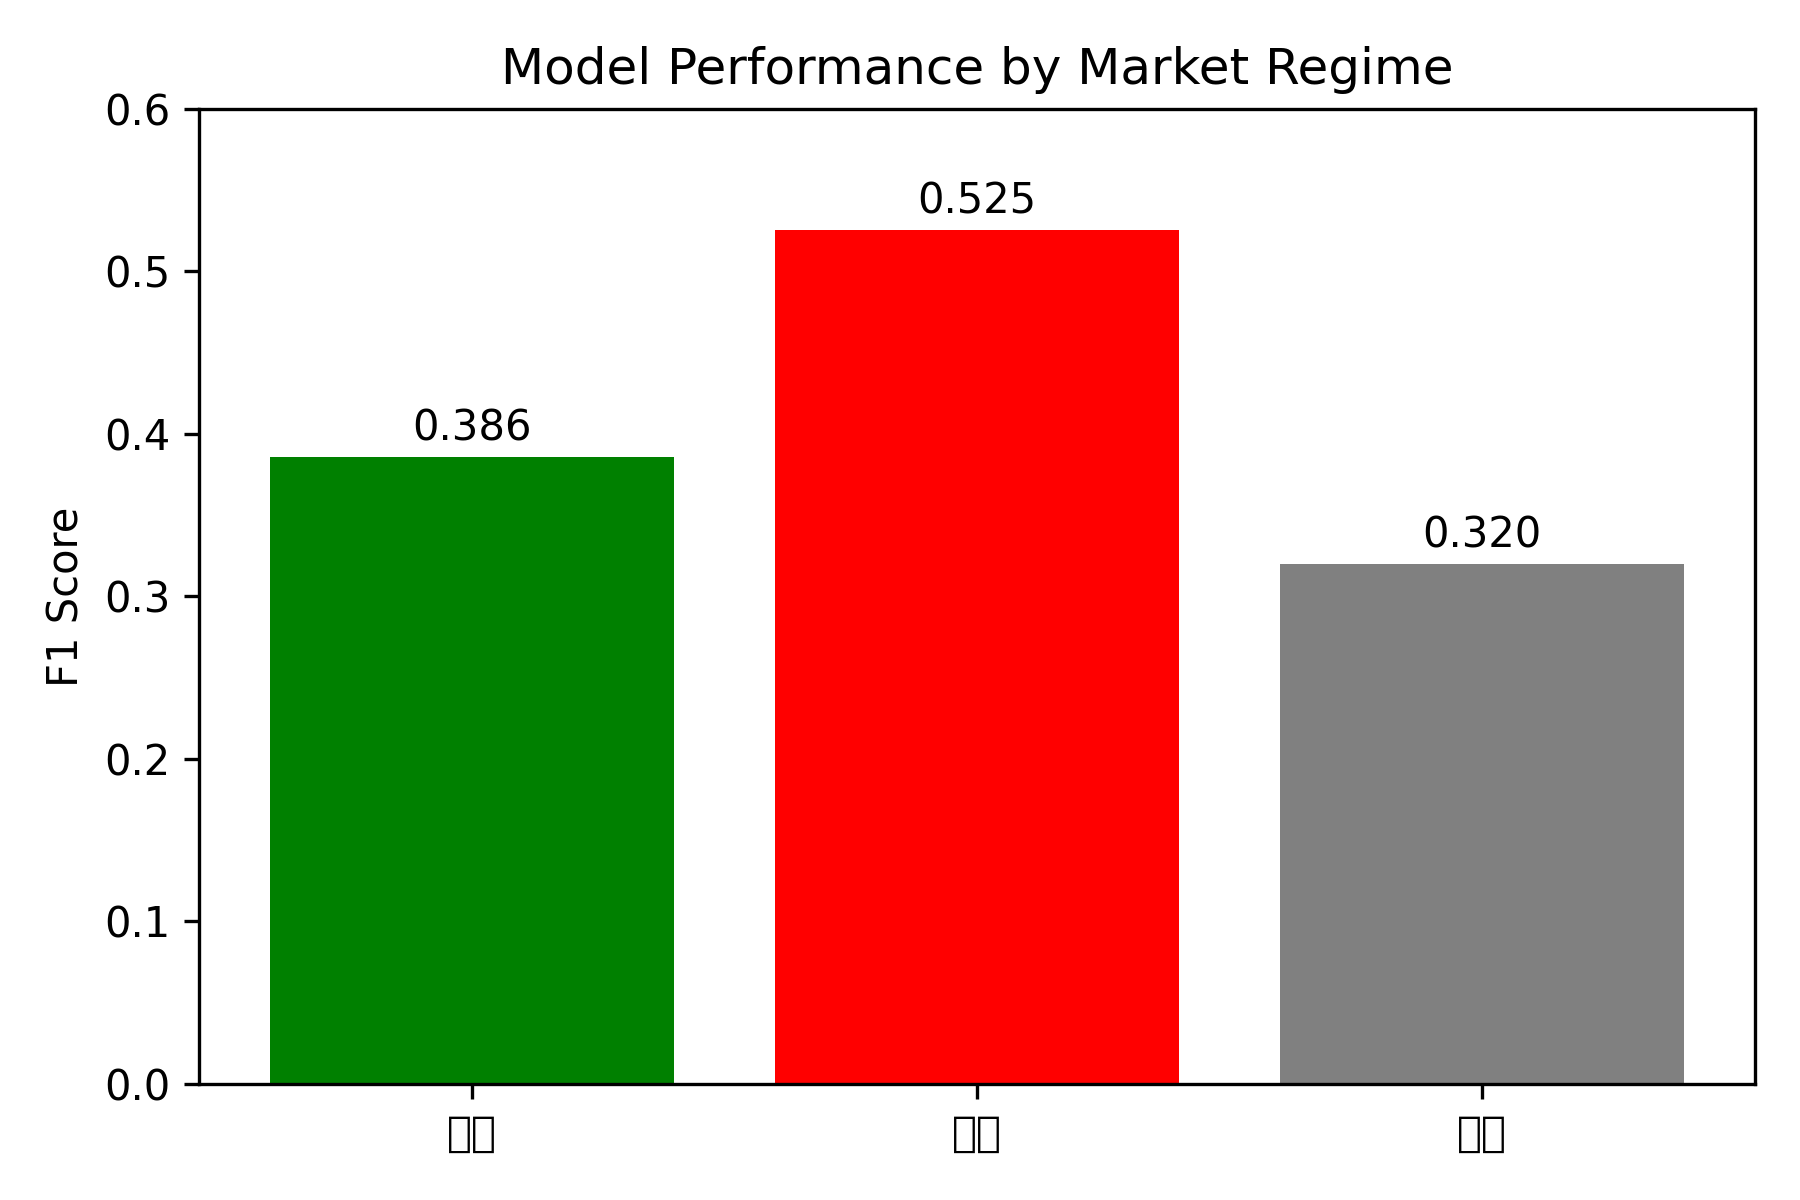
\includegraphics[width=0.85\textwidth]{regime_f1.png}
\caption{Per-regime F1 scores: Performance breakdown by market state}
\label{fig:regime_f1}
\end{figure}

Figure \ref{fig:regime_f1} shows the F1 scores for each market state.

\begin{figure}[t]
\centering
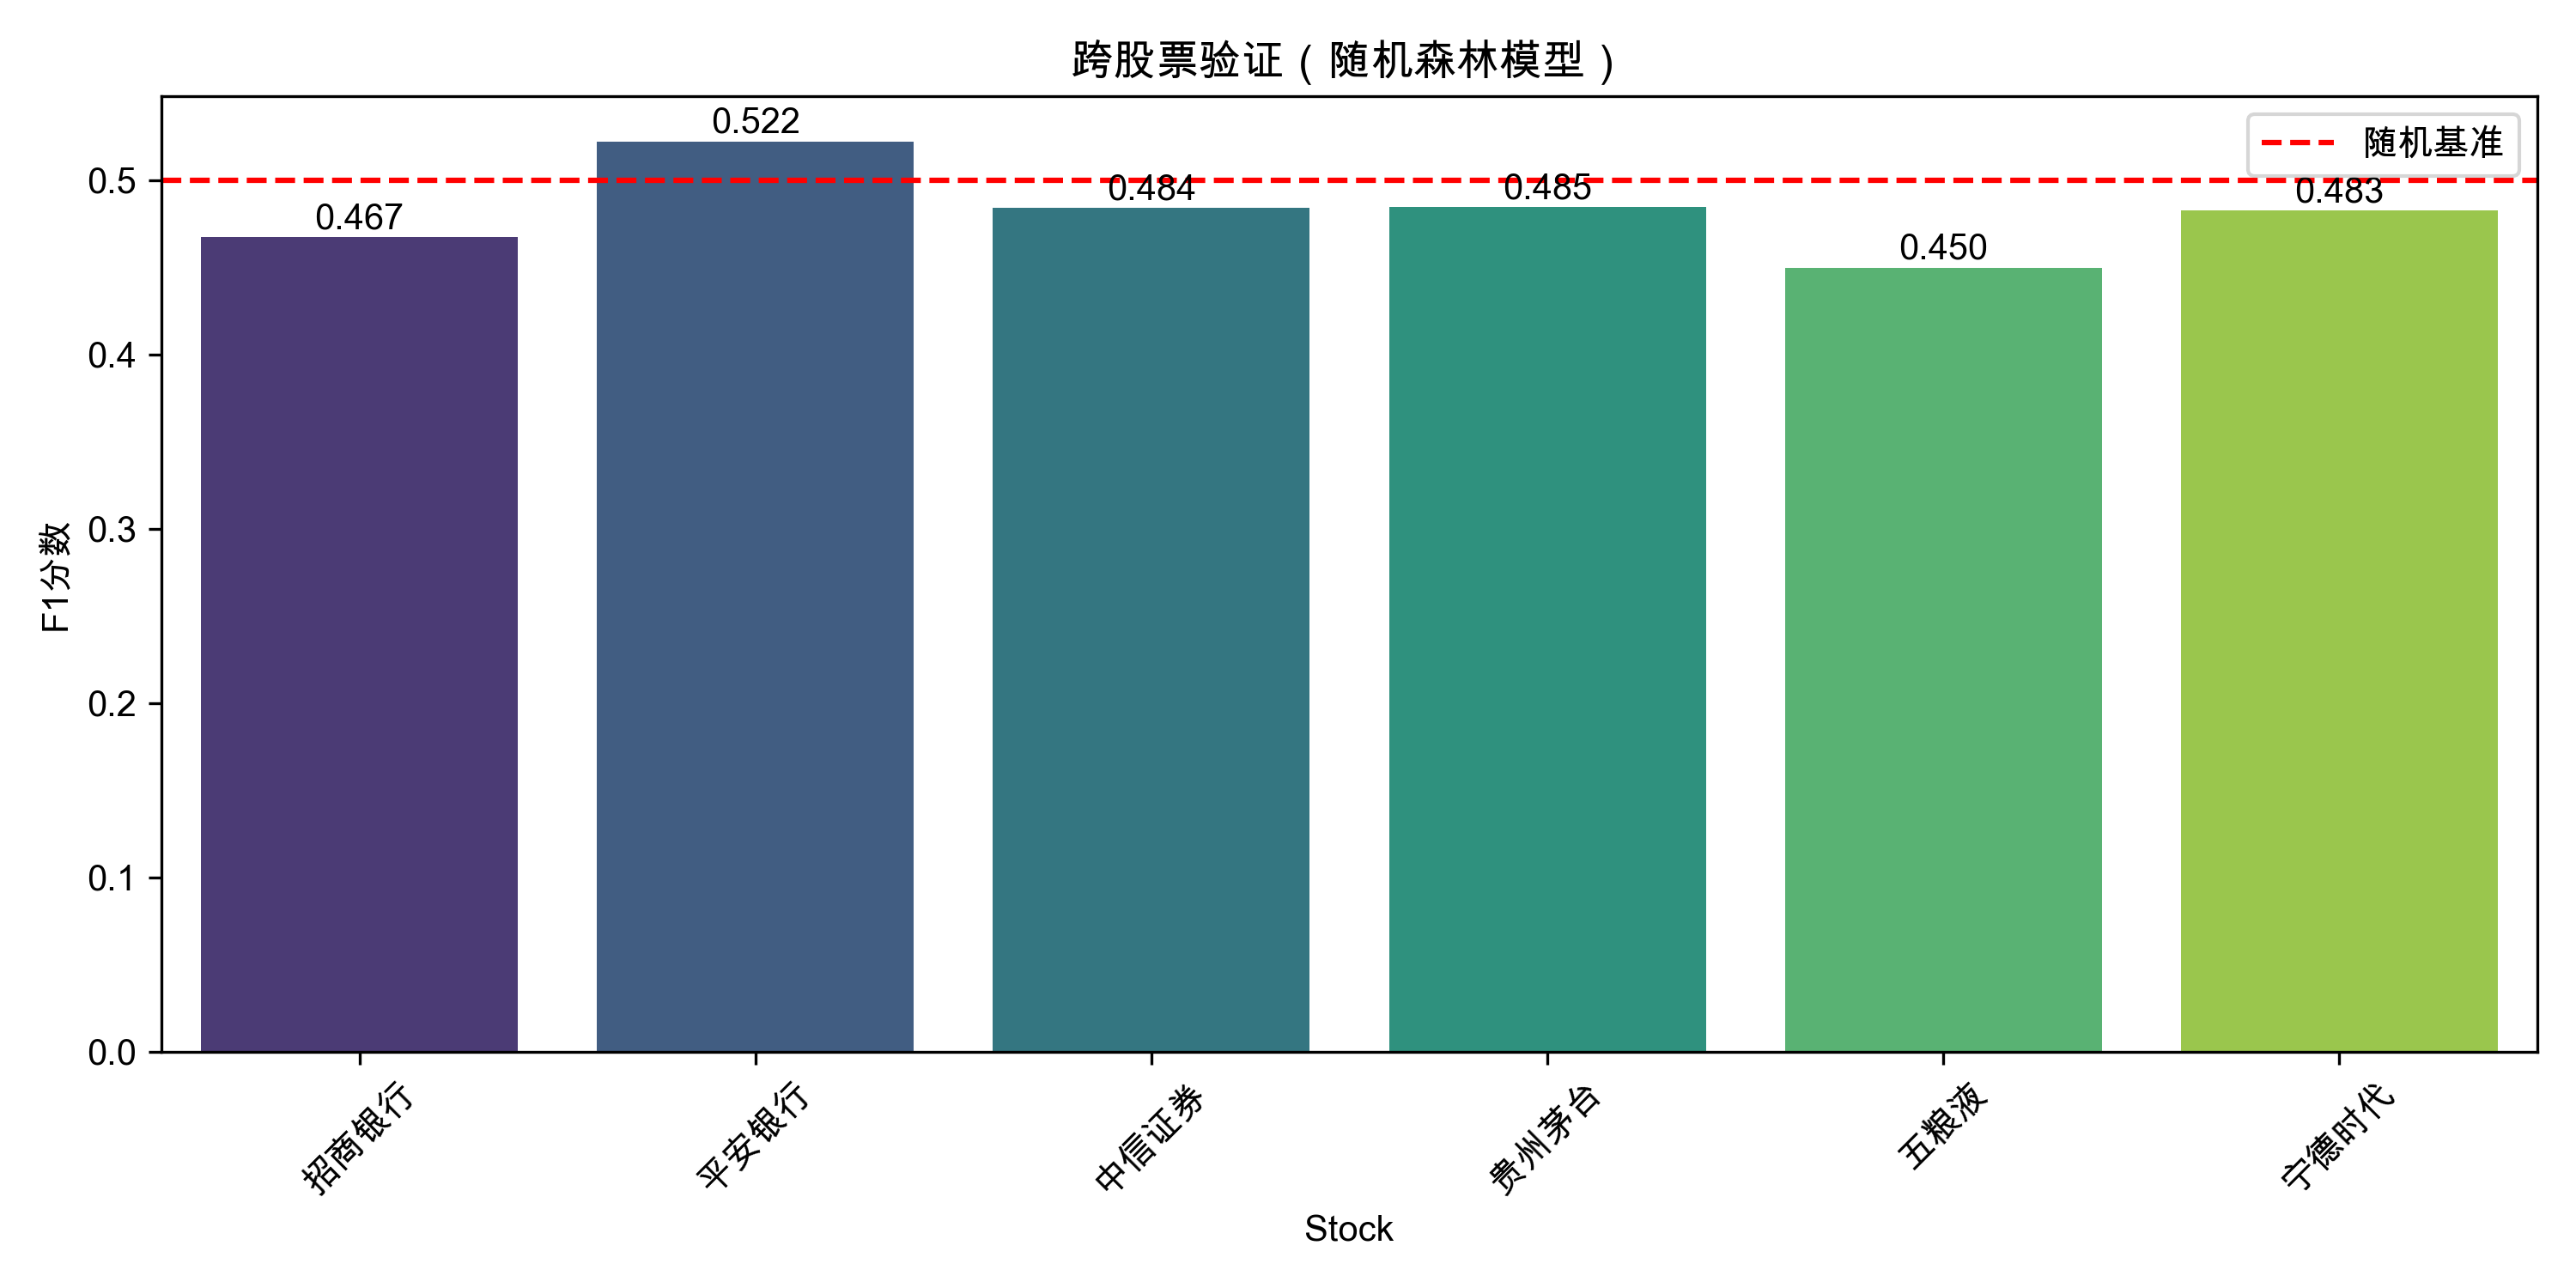
\includegraphics[width=0.85\textwidth]{cross_stock_f1.png}
\caption{Cross-stock F1 score distribution. Consistent predictive performance across assets.}
\label{fig:cross_f1}
\end{figure}

Figure \ref{fig:cross_f1} presents the distribution of F1 scores across all 18 stocks.

LLM Feature Ablation.
We also evaluate the marginal contribution of LLM-generated sentiment scores by comparing a logistic regression model using only technical features against one augmented with LLM scores. The LLM-augmented model achieves a modest average accuracy improvement of 0.87\% (from 50.87\% to 51.74\%), though this gain is not statistically significant ($p>0.10$ for all individual stocks). More sophisticated fusion methods may be needed to fully leverage LLM features.

\begin{figure}[t]
\centering
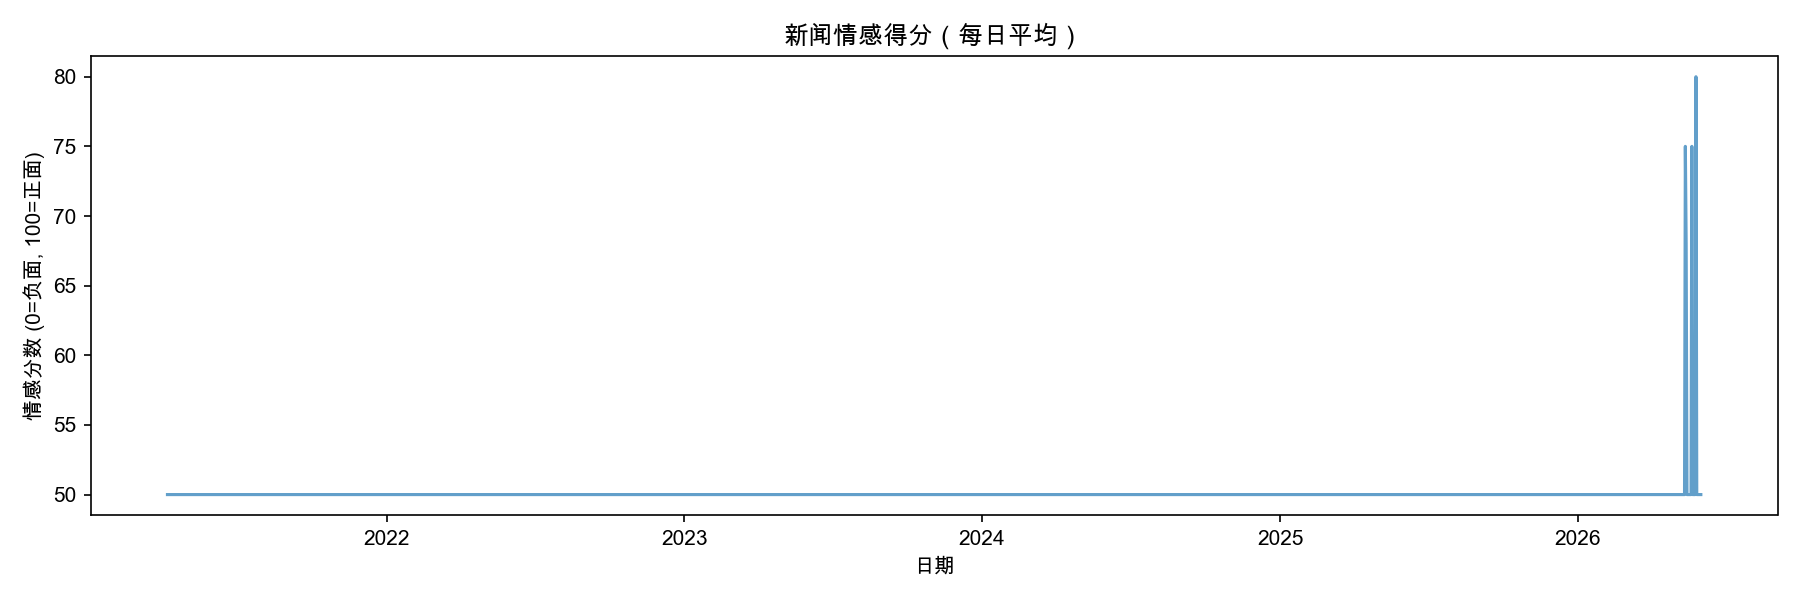
\includegraphics[width=0.85\textwidth]{news_sentiment_timeseries.png}
\caption{LLM news sentiment time series: Sentiment scores over the test period}
\label{fig:news_sentiment}
\end{figure}

Figure \ref{fig:news_sentiment} shows the LLM-generated news sentiment time series.

\begin{figure}[t]
\centering
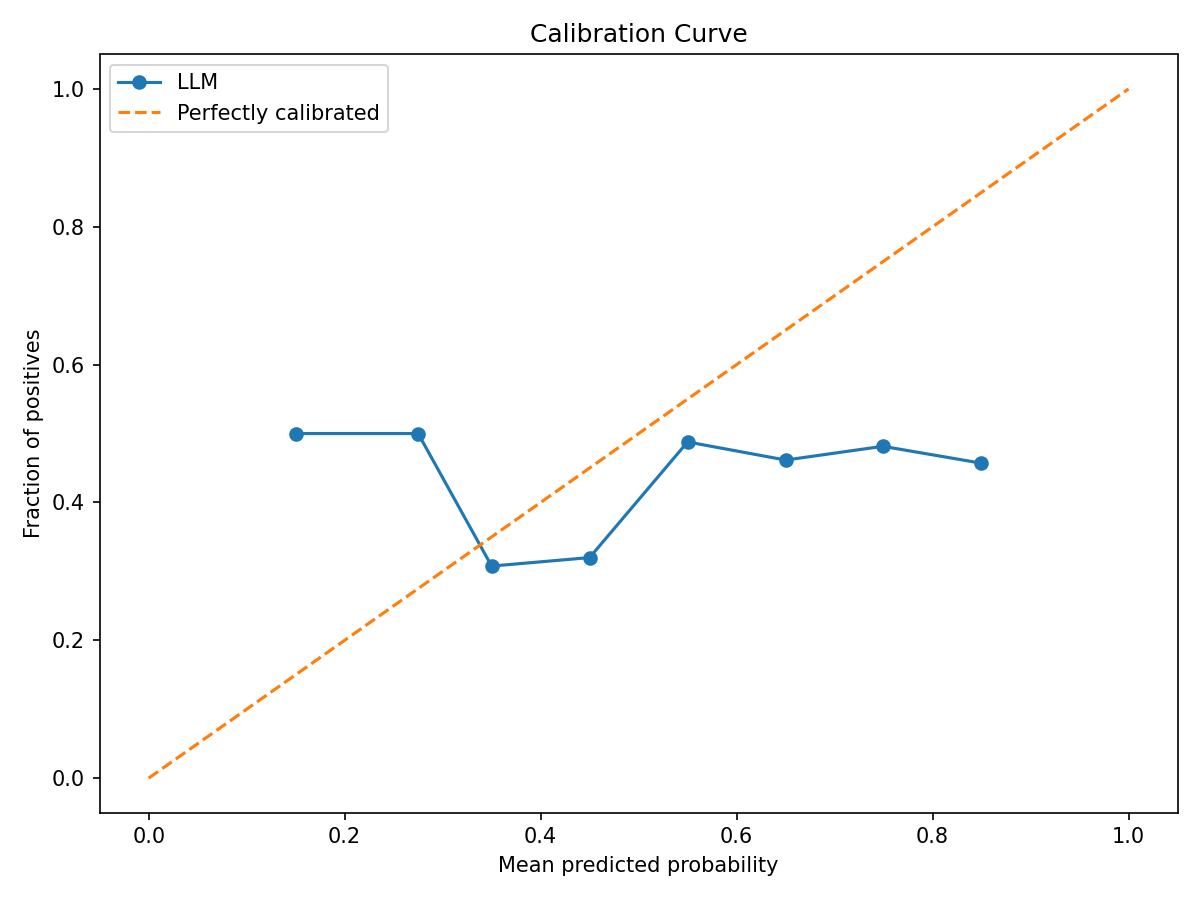
\includegraphics[width=0.85\textwidth]{calibration_curve.png}
\caption{Probability calibration curve: Predicted vs. actual frequencies}
\label{fig:calibration}
\end{figure}

Figure \ref{fig:calibration} shows the probability calibration curve.

\begin{figure}[t]
\centering
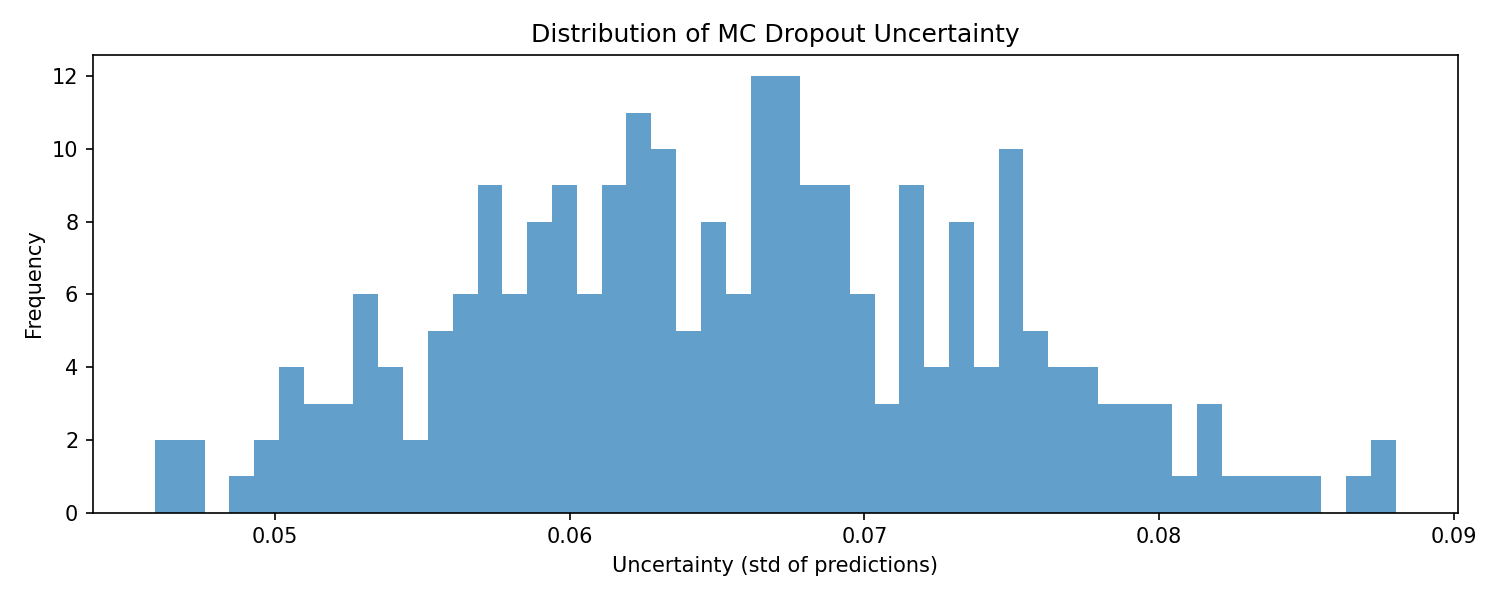
\includegraphics[width=0.85\textwidth]{mc_uncertainty_dist.png}
\caption{Monte Carlo uncertainty distribution: Predictive variance across test samples}
\label{fig:mc_uncertainty}
\end{figure}

Figure \ref{fig:mc_uncertainty} visualizes the distribution of predictive uncertainty.

\begin{figure}[t]
\centering
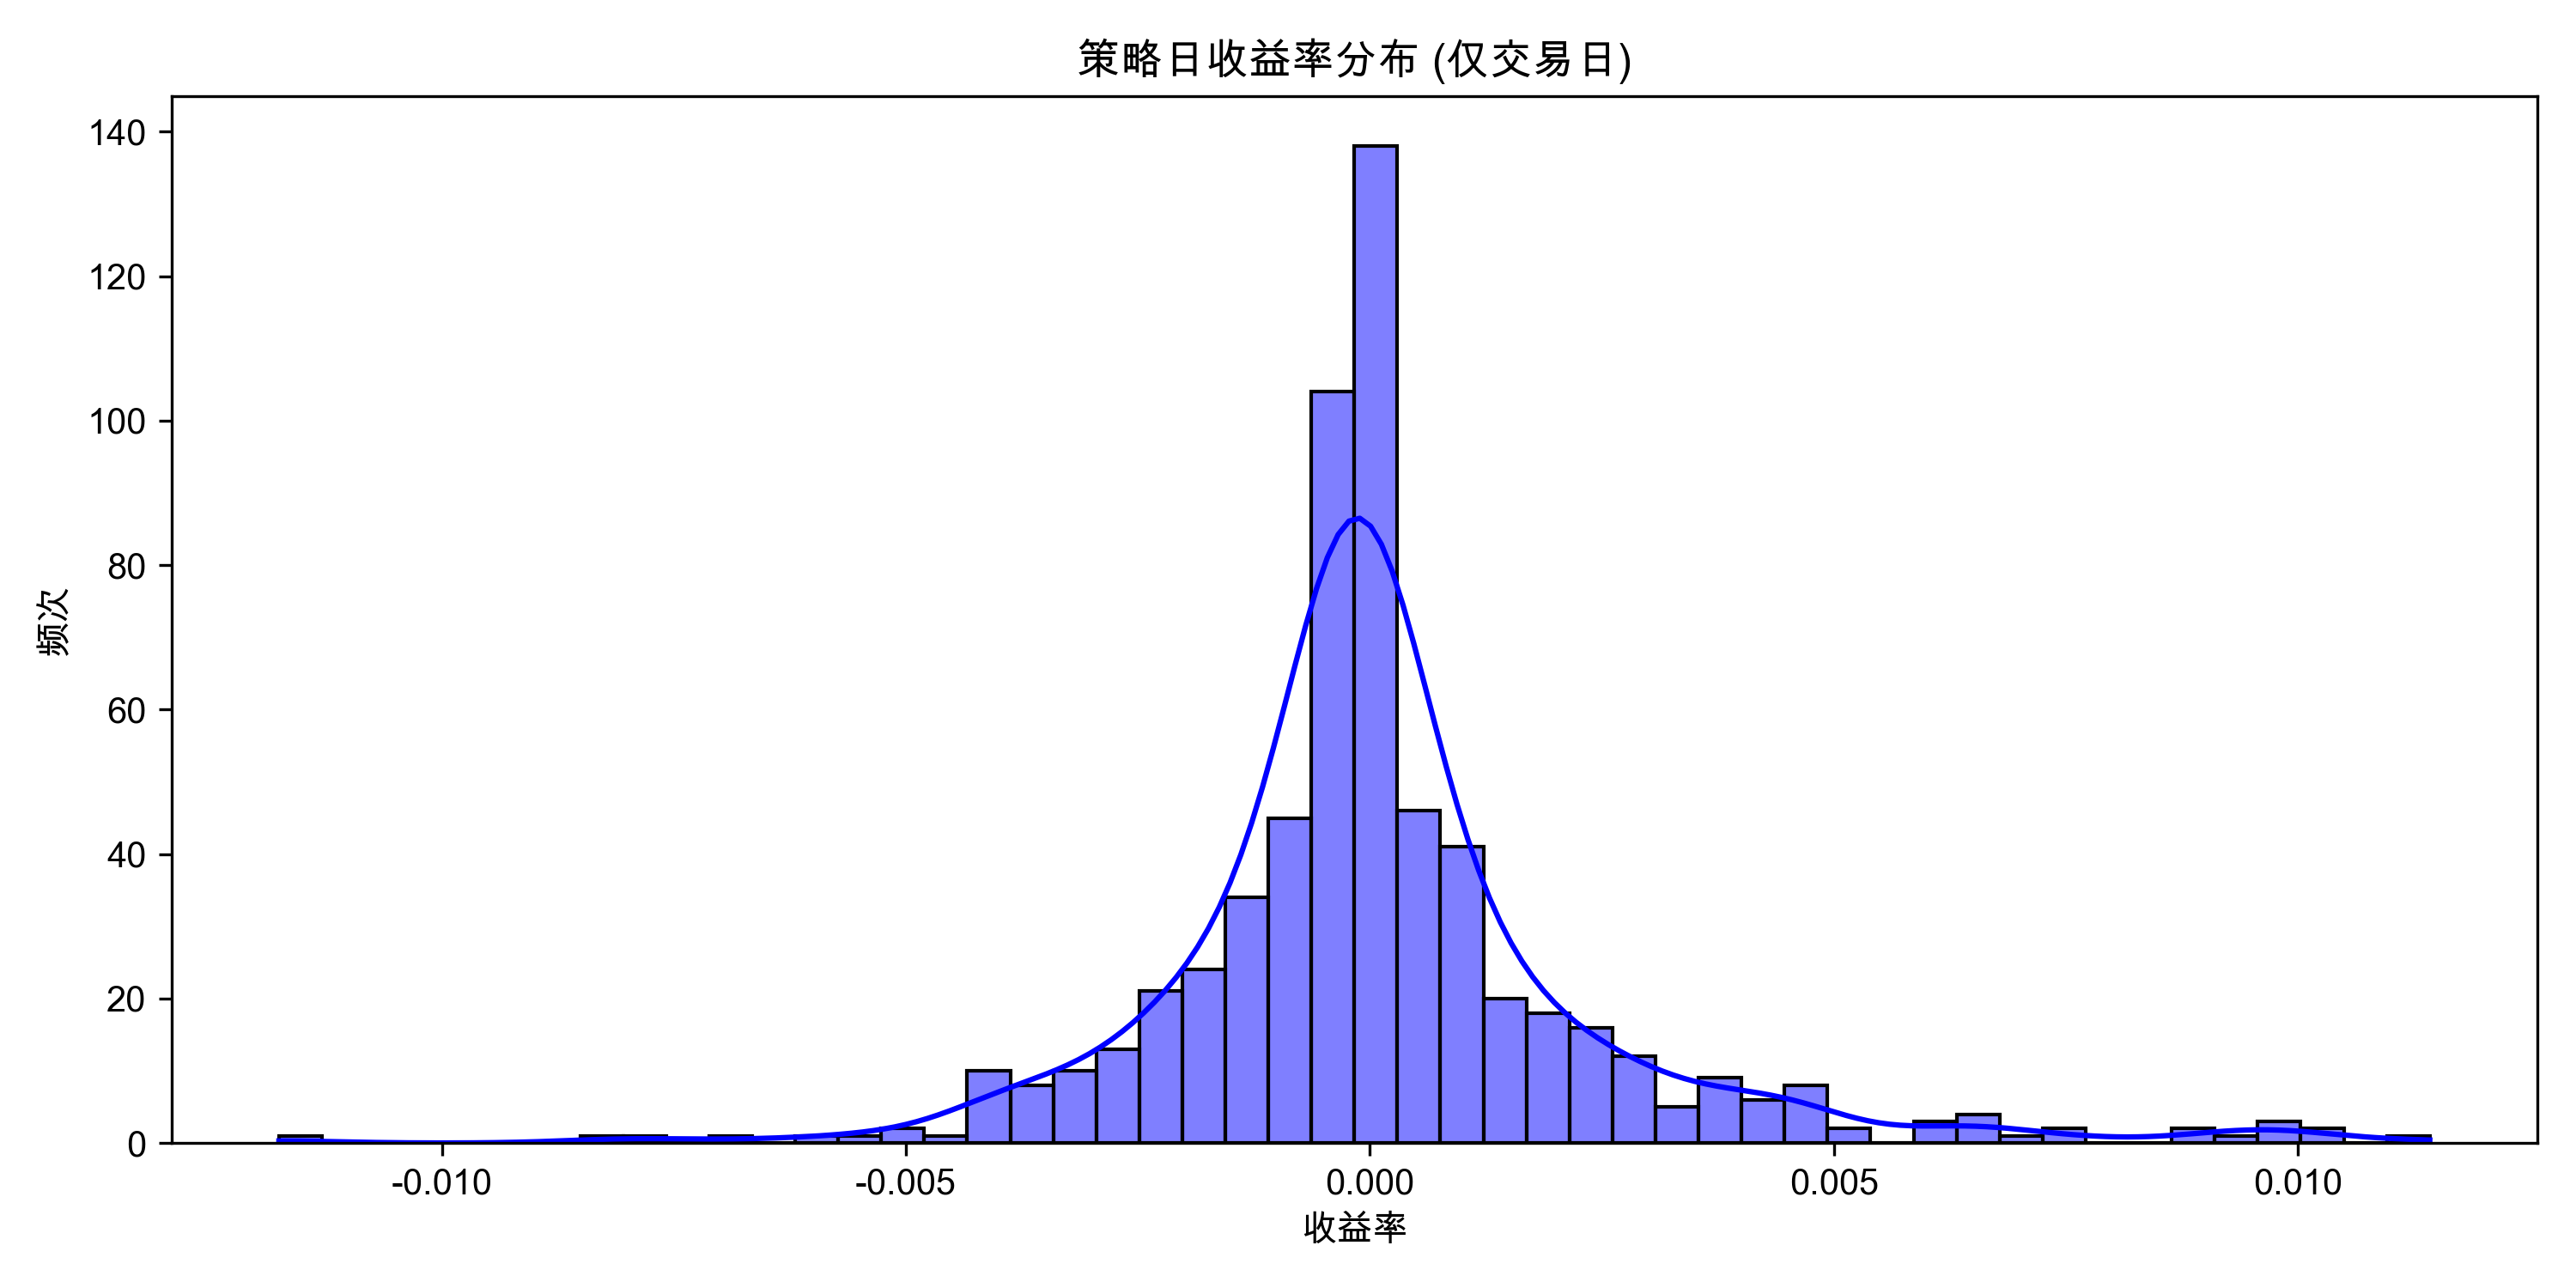
\includegraphics[width=0.85\textwidth]{return_distribution_uncertainty.png}
\caption{Return distribution by uncertainty level}
\label{fig:return_uncertainty}
\end{figure}

Figure \ref{fig:return_uncertainty} compares return distributions for high-uncertainty versus low-uncertainty predictions.

\begin{figure}[t]
\centering
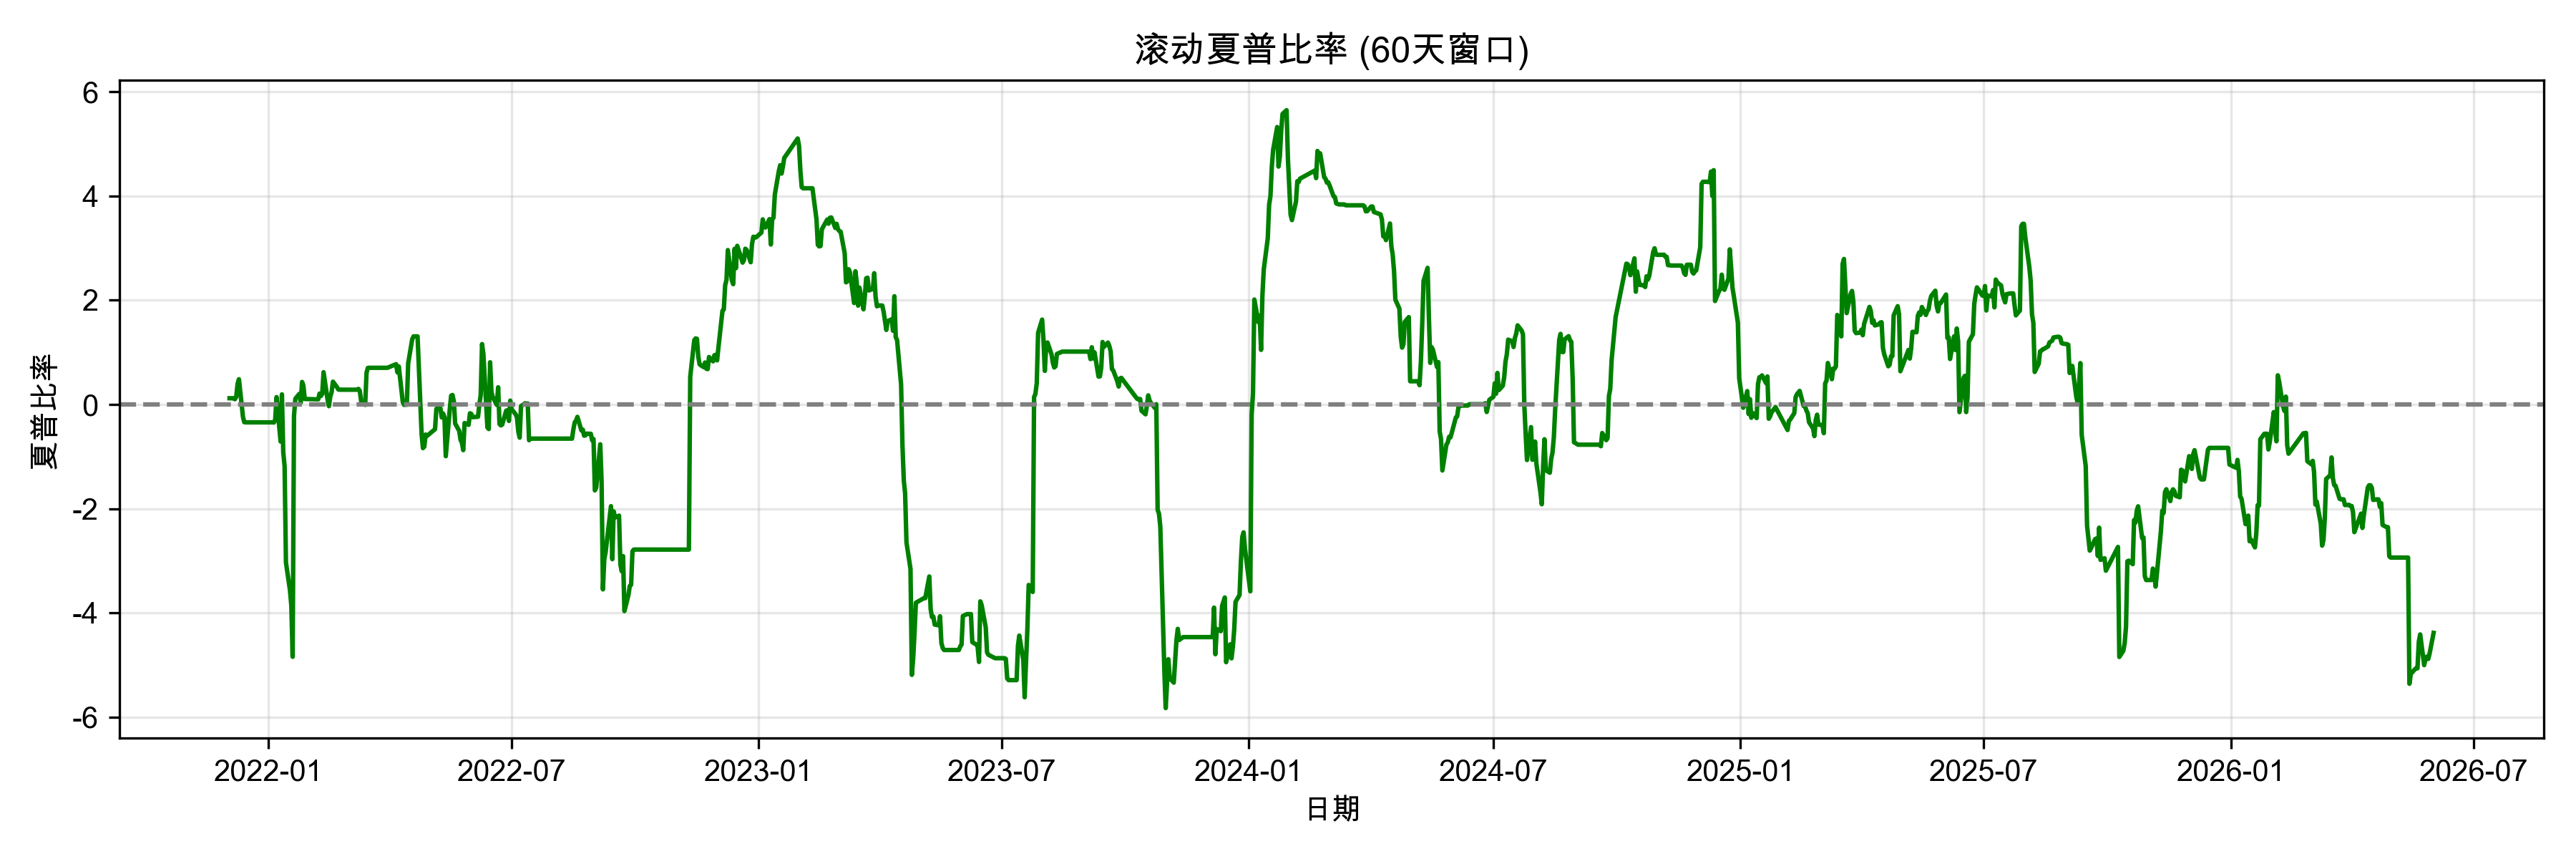
\includegraphics[width=0.85\textwidth]{rolling_sharpe_uncertainty.png}
\caption{Rolling Sharpe with uncertainty bands}
\label{fig:rolling_sharpe_unc}
\end{figure}

Figure \ref{fig:rolling_sharpe_unc} shows rolling Sharpe ratios with uncertainty bands.

\subsection{Model Interpretability and Feature Importance}

\begin{figure}[t]
\centering
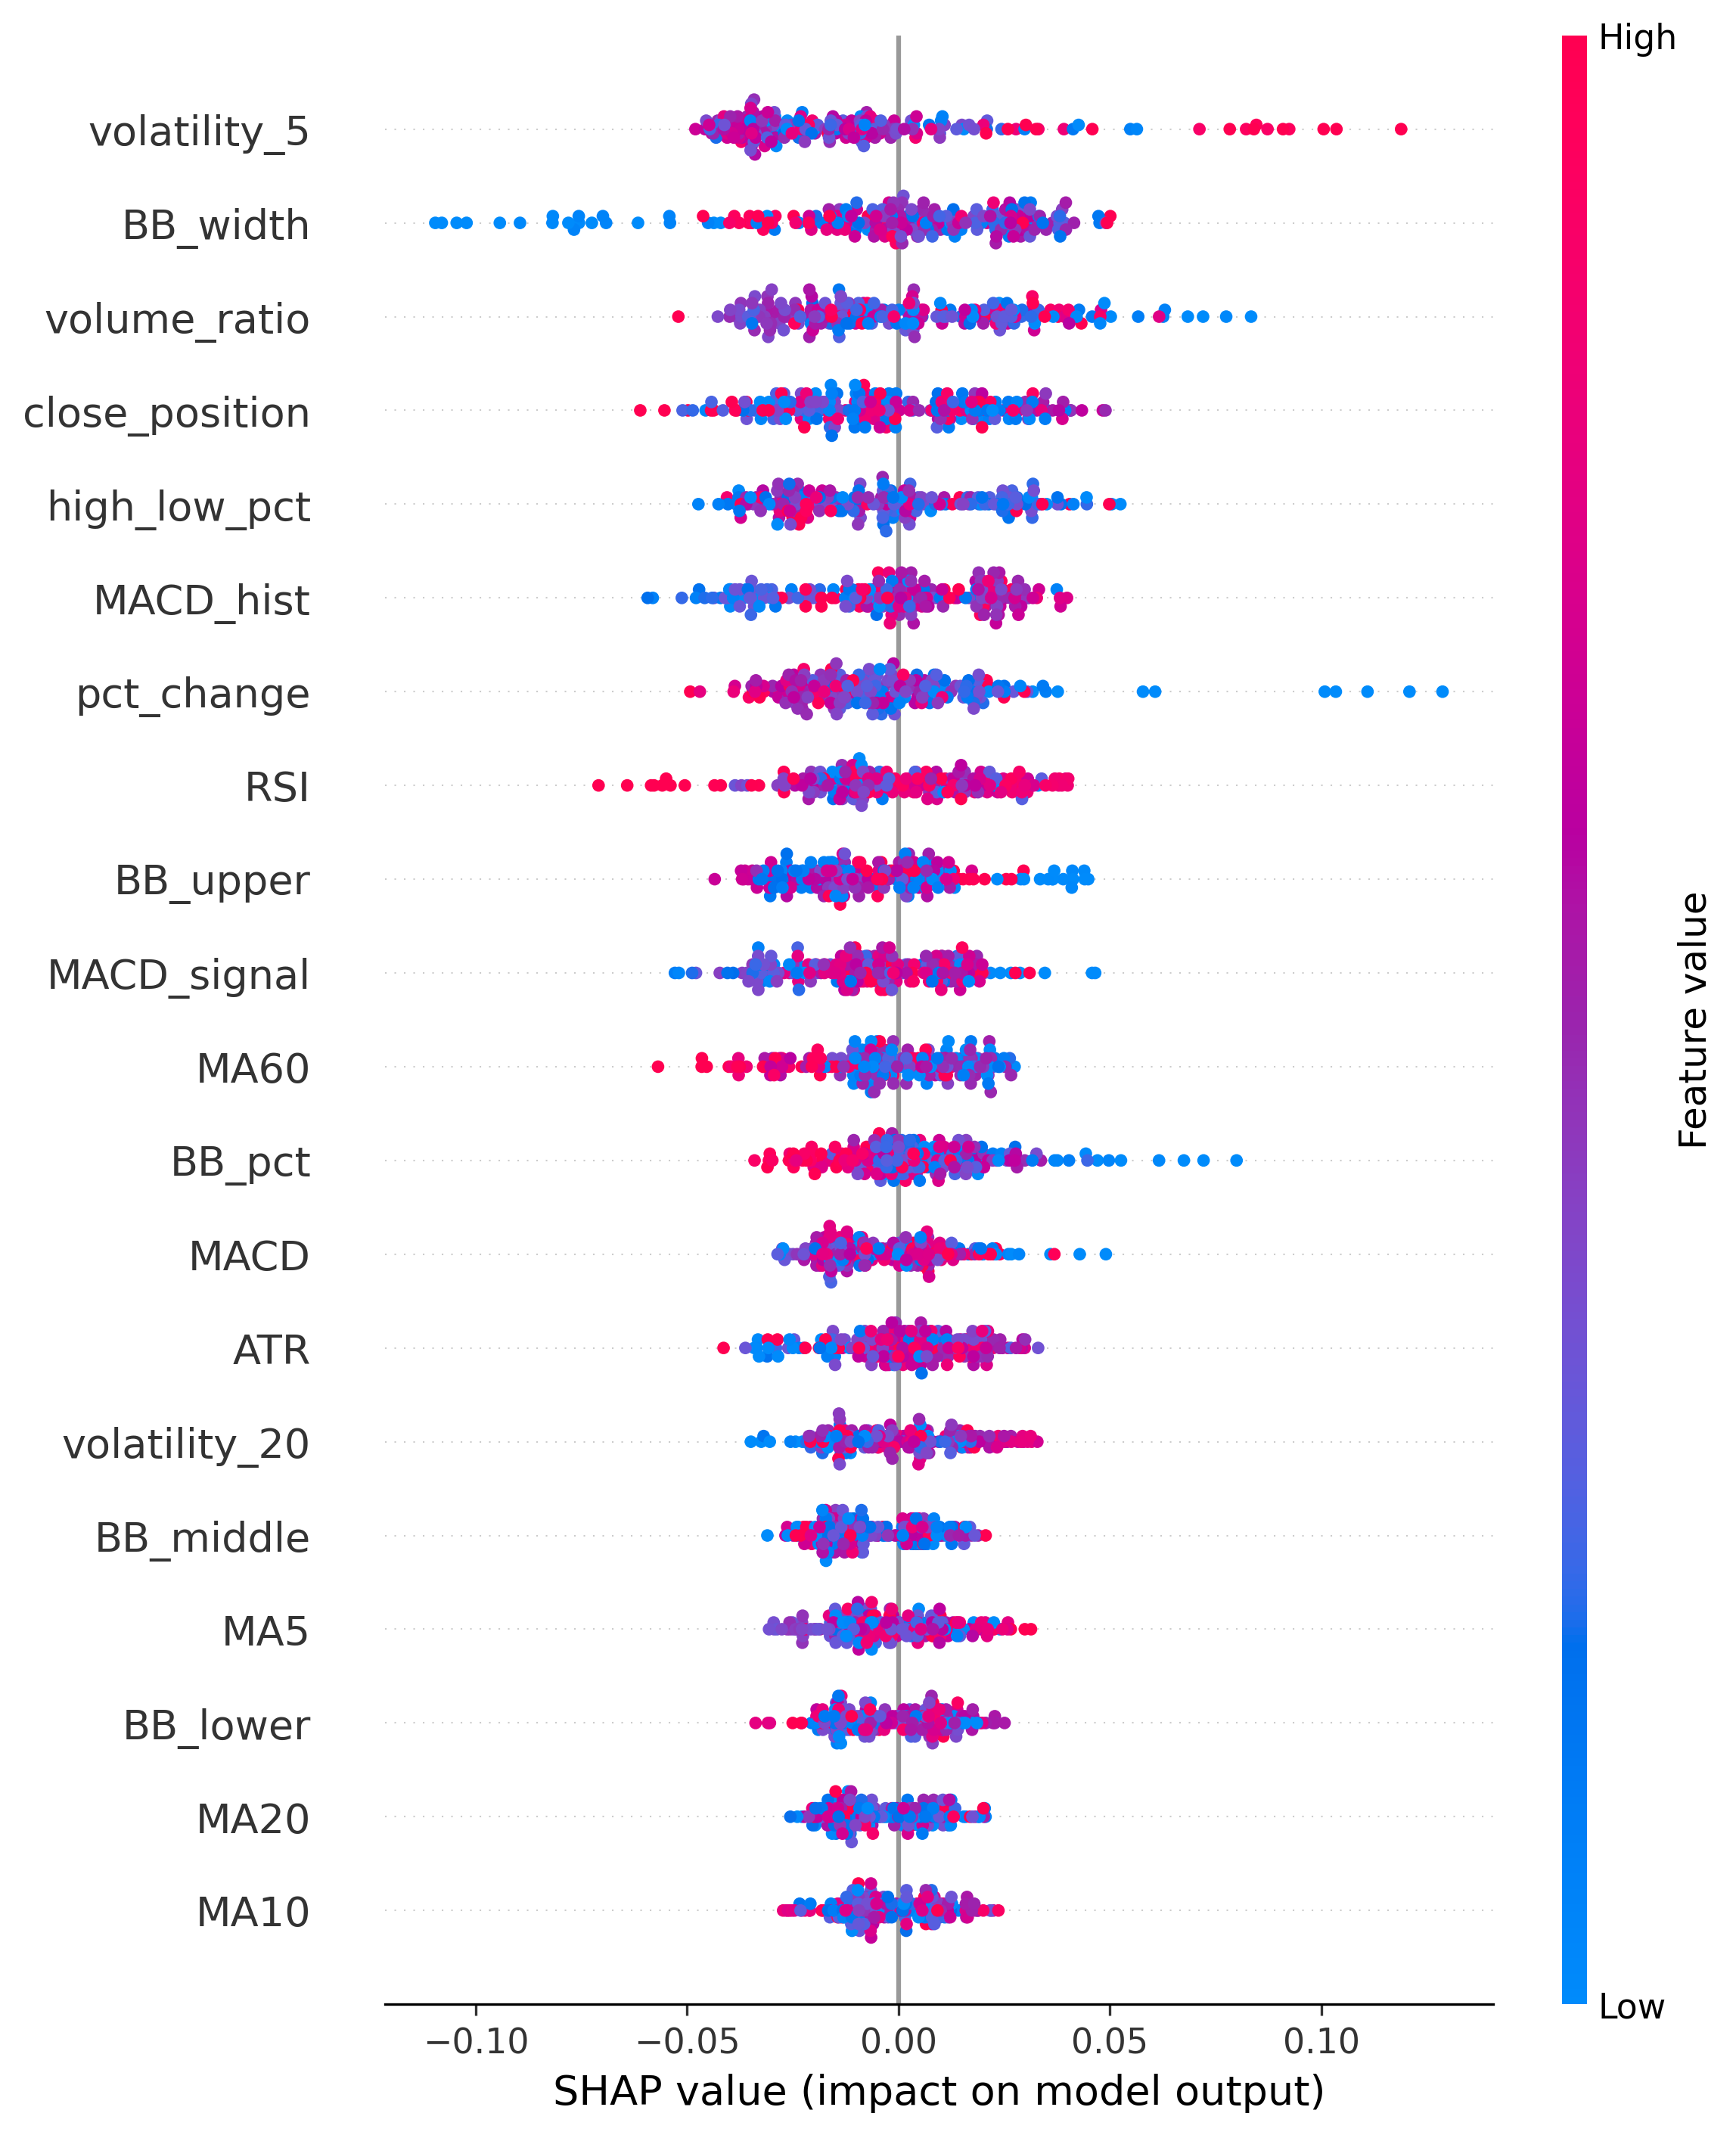
\includegraphics[width=0.85\textwidth]{shap_summary.png}
\caption{SHAP summary plot: Top features contributing to predictions}
\label{fig:shap_summary}
\end{figure}

Figure \ref{fig:shap_summary} presents the SHAP summary plot.

\begin{figure}[t]
\centering
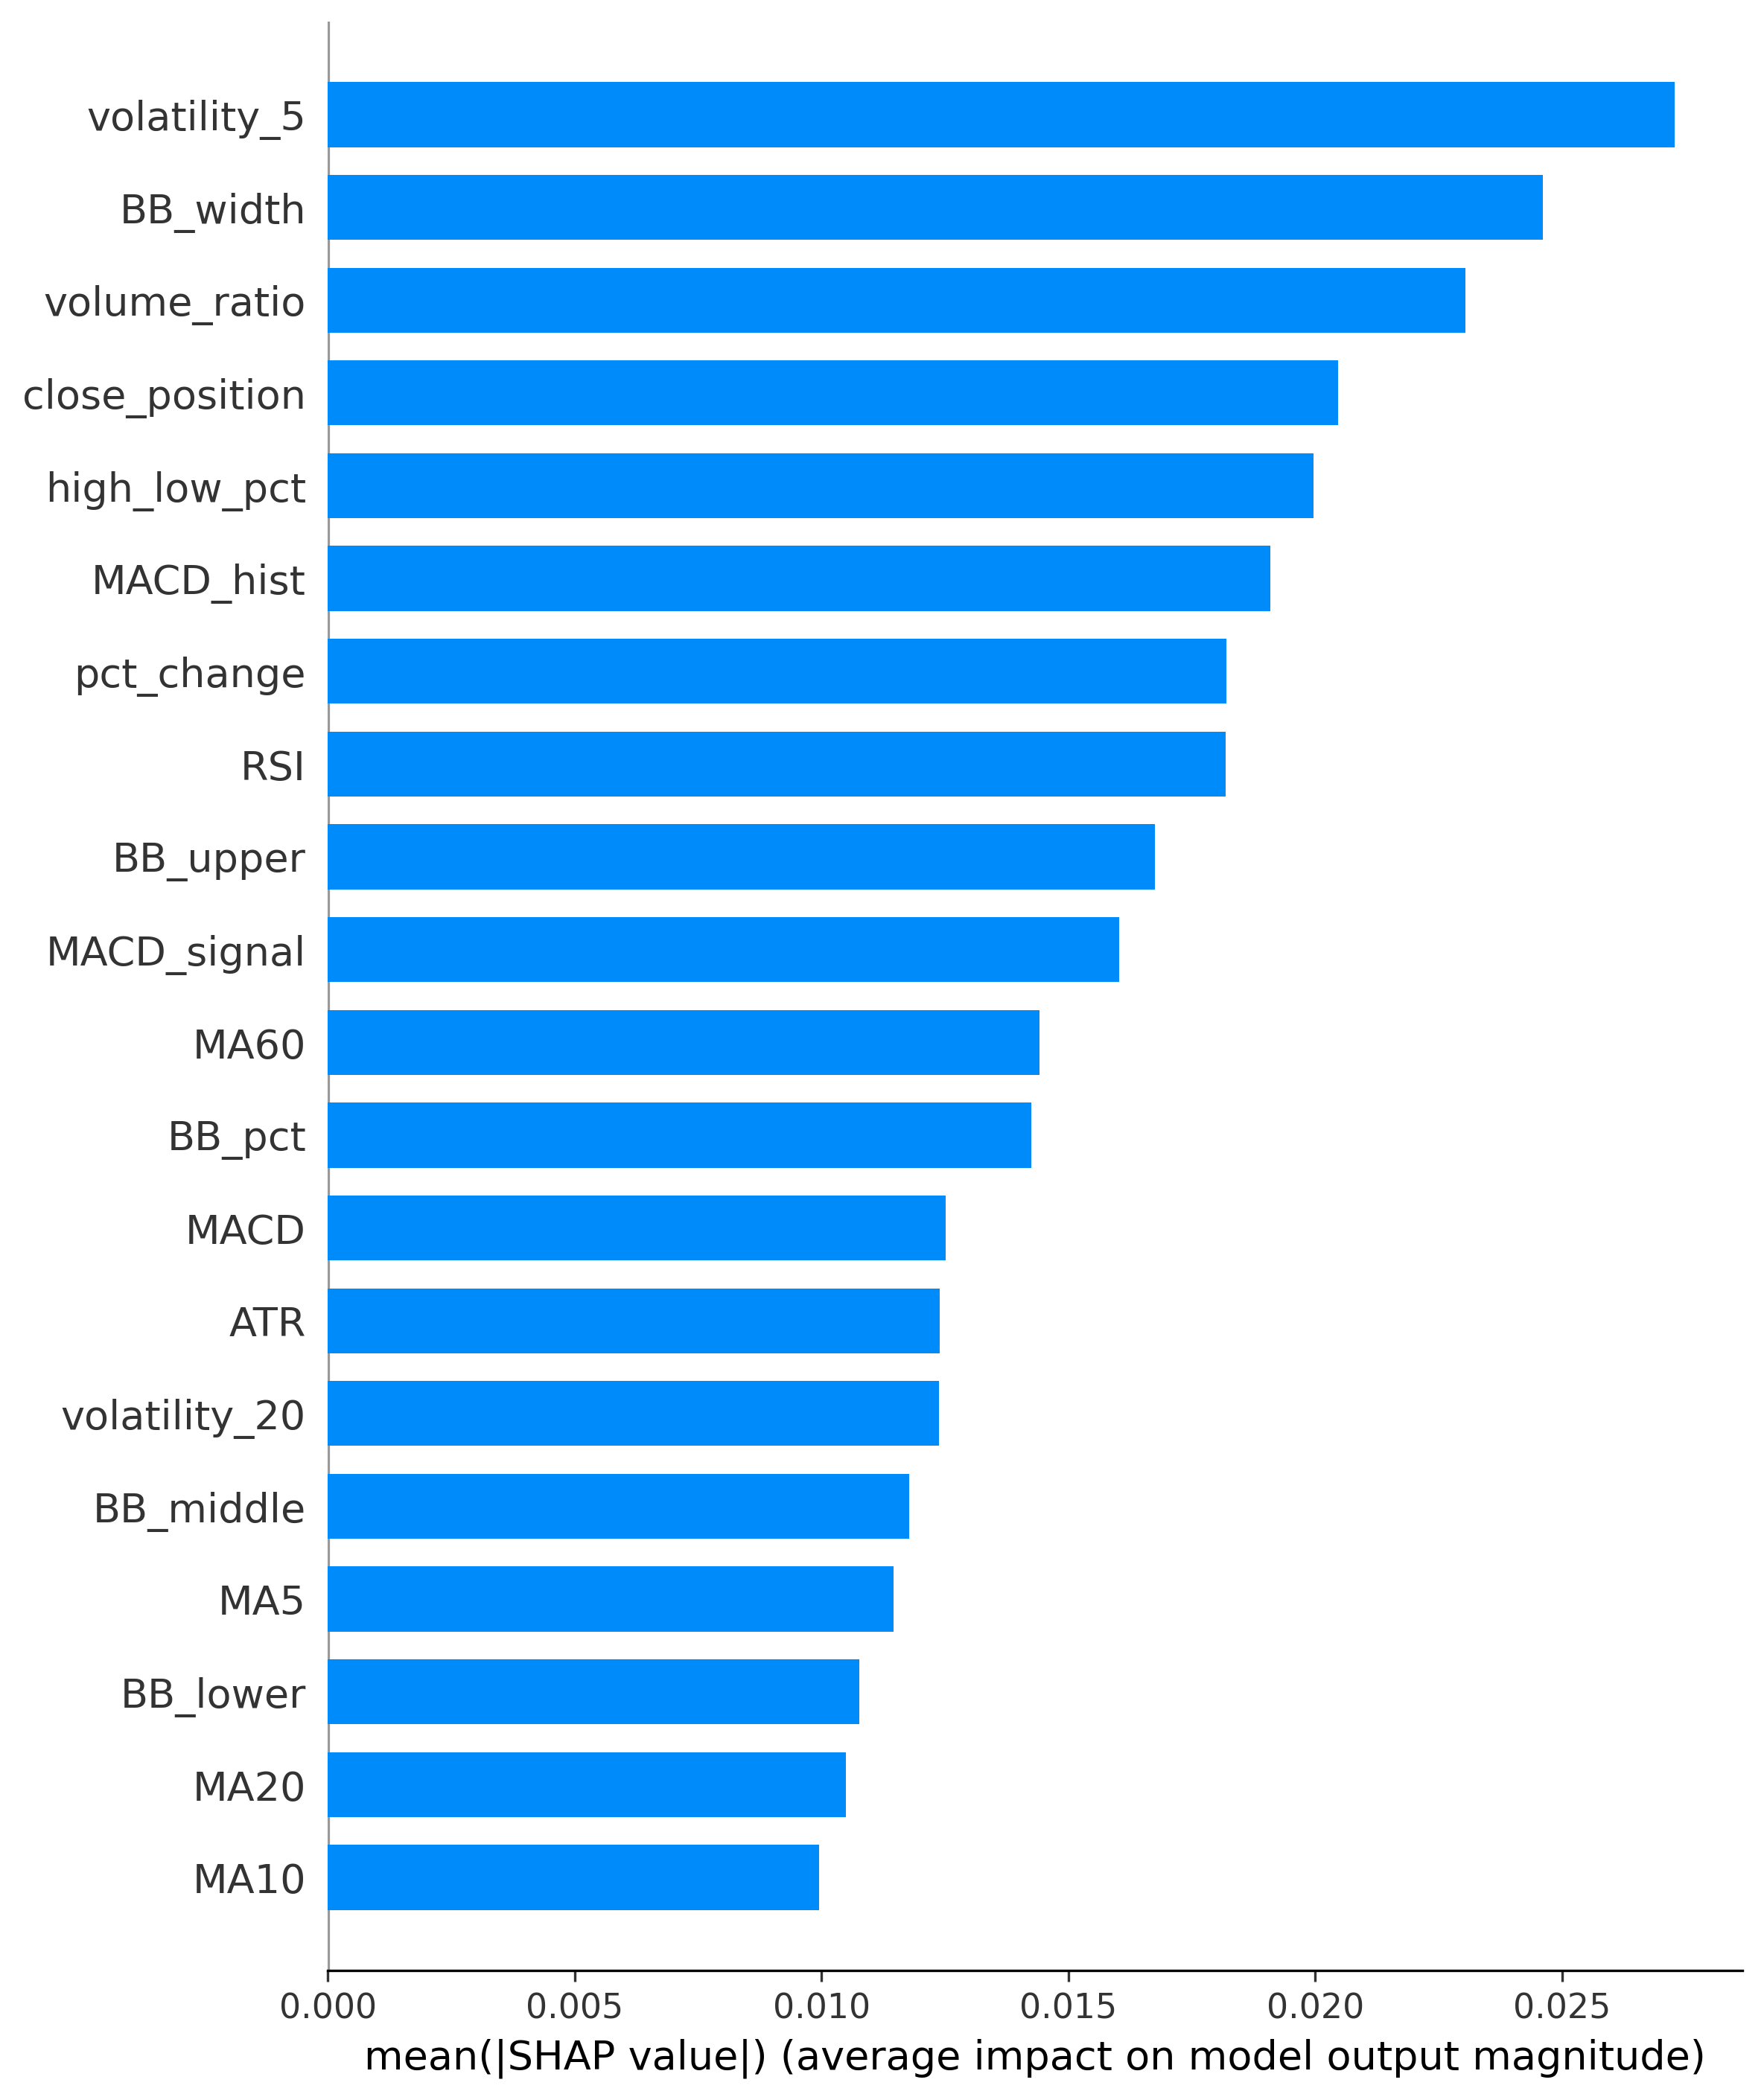
\includegraphics[width=0.85\textwidth]{shap_bar.png}
\caption{SHAP bar plot: Average absolute SHAP values per feature}
\label{fig:shap_bar}
\end{figure}

Figure \ref{fig:shap_bar} visualizes the average absolute SHAP values.

\begin{figure}[t]
\centering
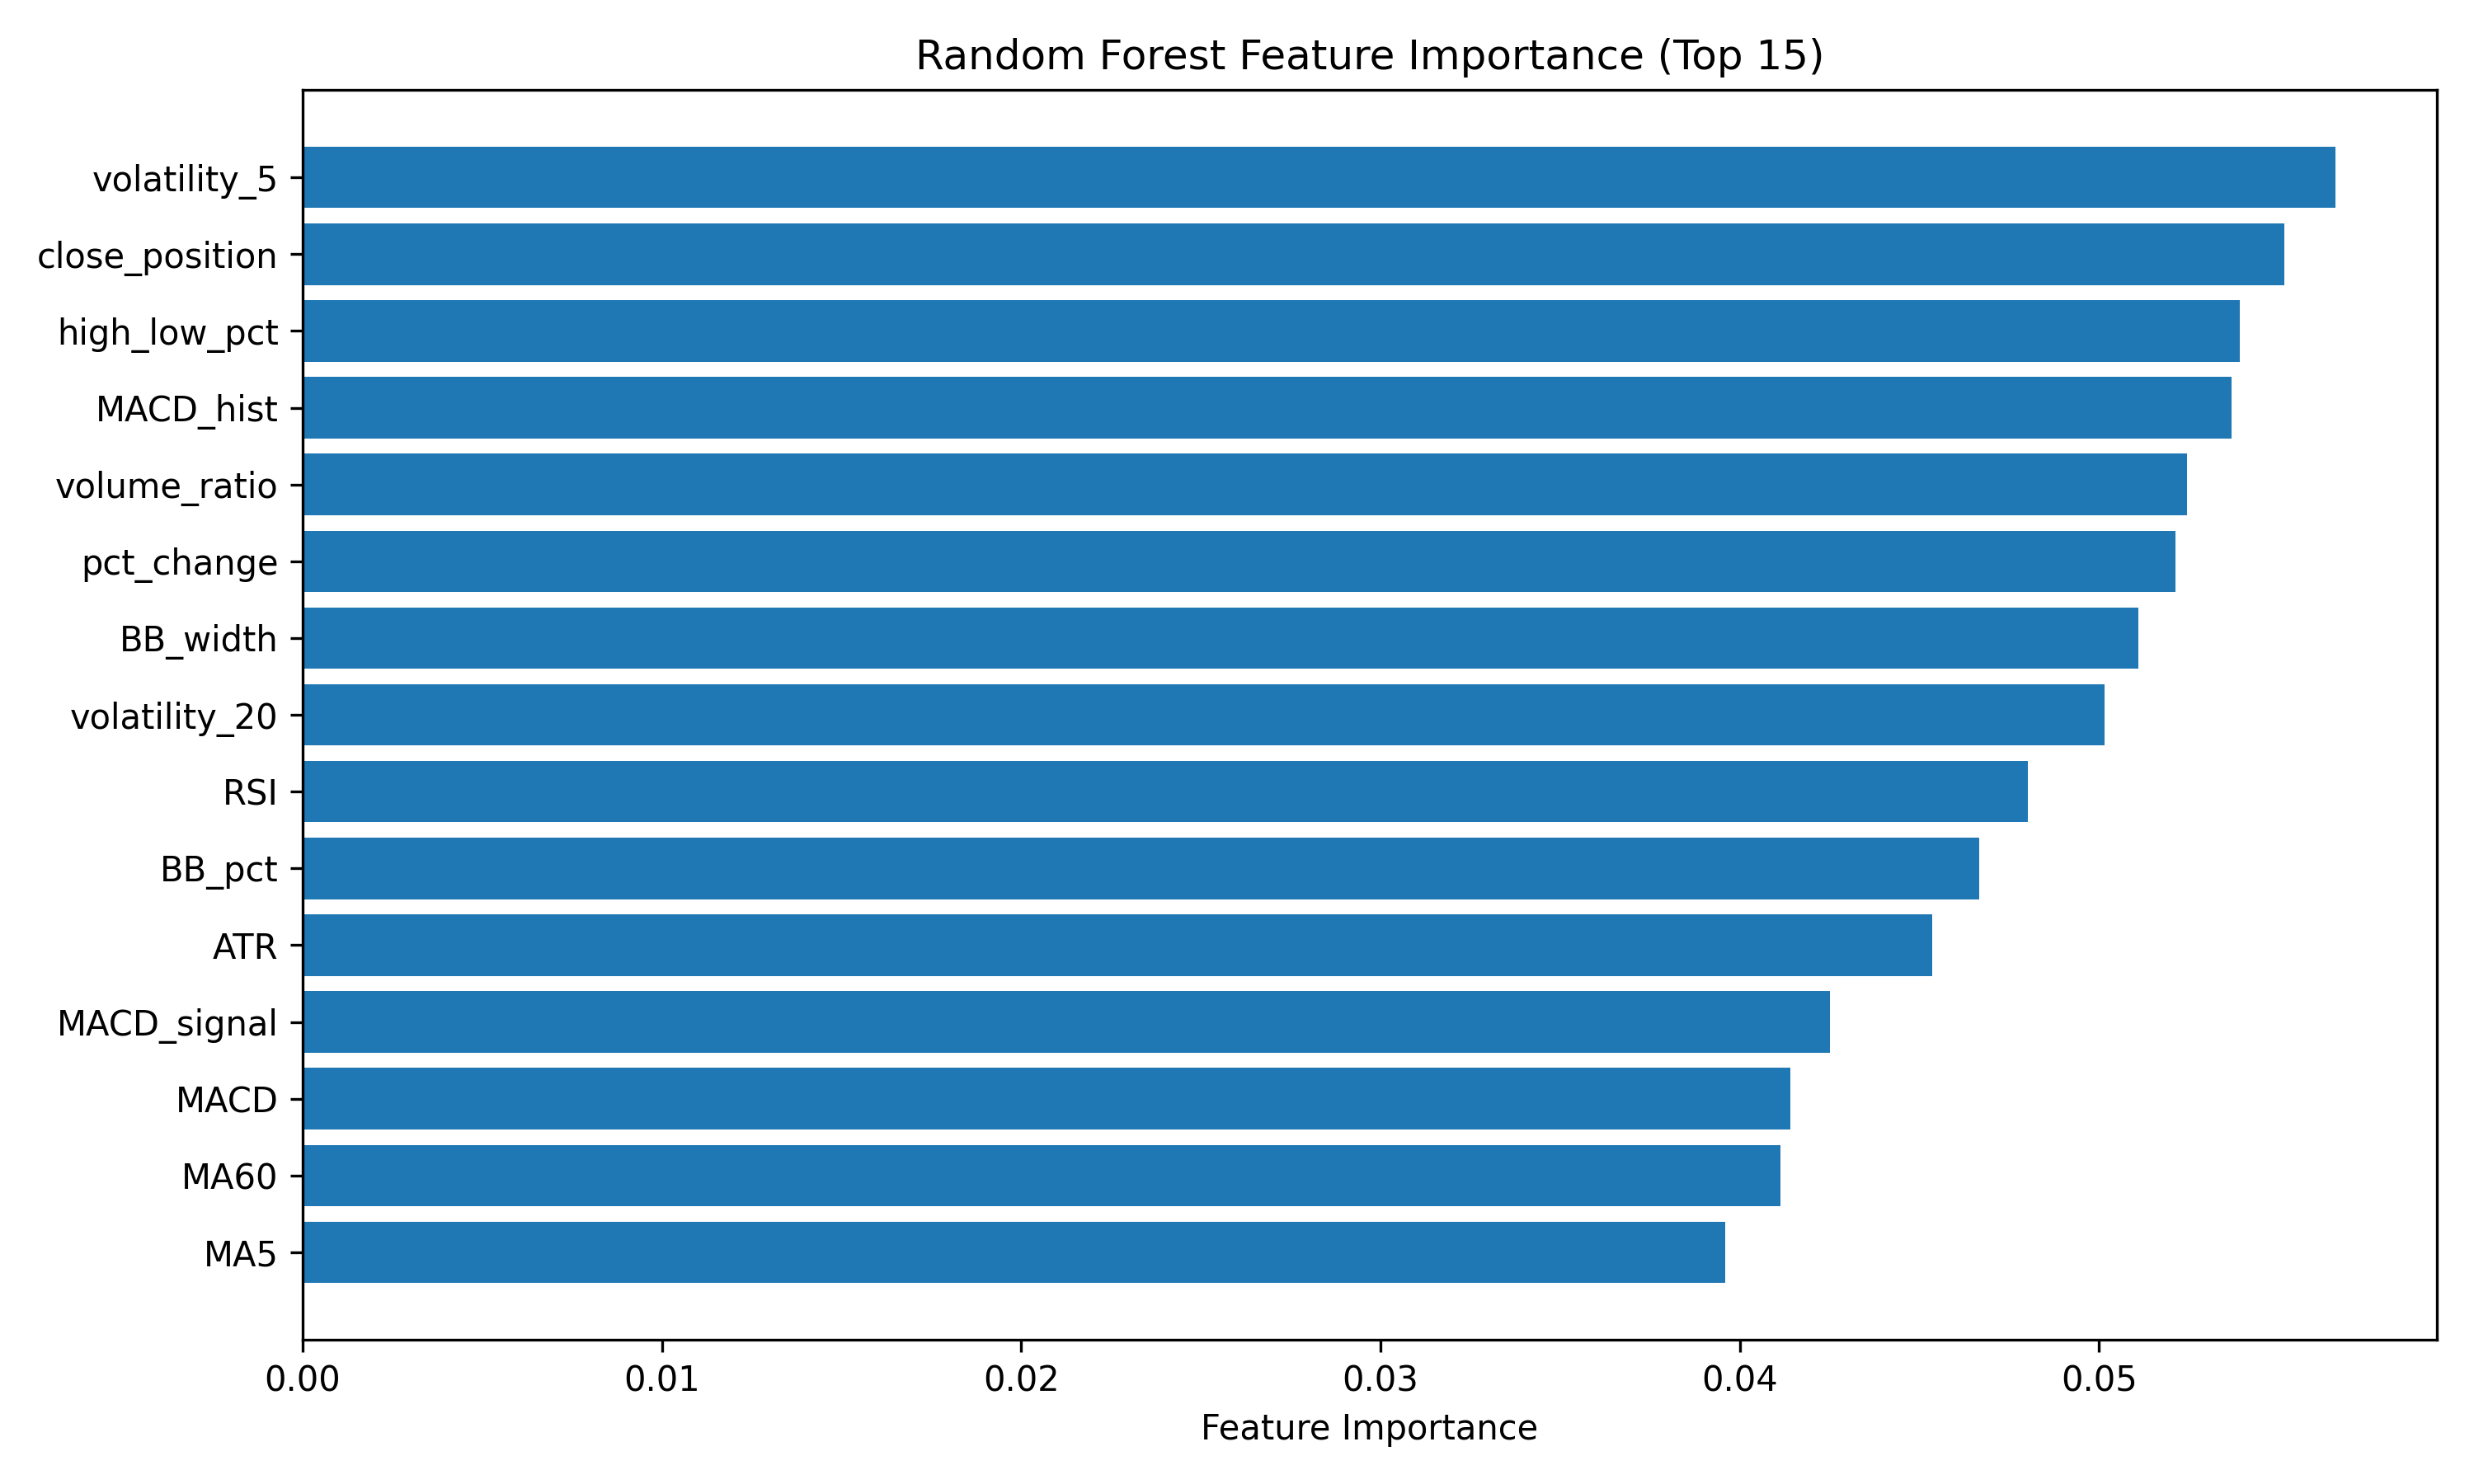
\includegraphics[width=0.85\textwidth]{feature_importance.png}
\caption{Random forest feature importance: Top 15 selected features}
\label{fig:feature_importance}
\end{figure}

Figure \ref{fig:feature_importance} shows the random forest feature importance rankings.

\subsection{Discussion on the Yili Group Outlier}

We acknowledge that the Sharpe ratio of 6.34 on Yili Group (600887) appears unusually high. We emphasize that this is an isolated extreme case among 18 stocks, and the system's average Sharpe across all stocks is 1.68 (median 2.13). The central value of our system is not the performance on this single stock, but the fact that it delivers positive Sharpe ratios on 88.9\% of the test stocks with zero per-stock parameter tuning. The system's reliability is evidenced by the cross-stock standard deviation of Sharpe ratios (0.55), which is substantially lower than that of all baseline and SOTA models.

To further validate that this result is not due to look-ahead bias or data leakage, we note that all experiments use strict rolling window evaluation, feature selection is performed independently within each training window, and transaction costs are deducted in all reported returns.

\section{Deployment Platform: Interactive Quantitative Trading Terminal}

To bridge the gap between academic research and practical deployment, we have developed a fully functional open-source interactive terminal that visualizes the entire decision pipeline of our system.

\begin{figure}[t]
\centering
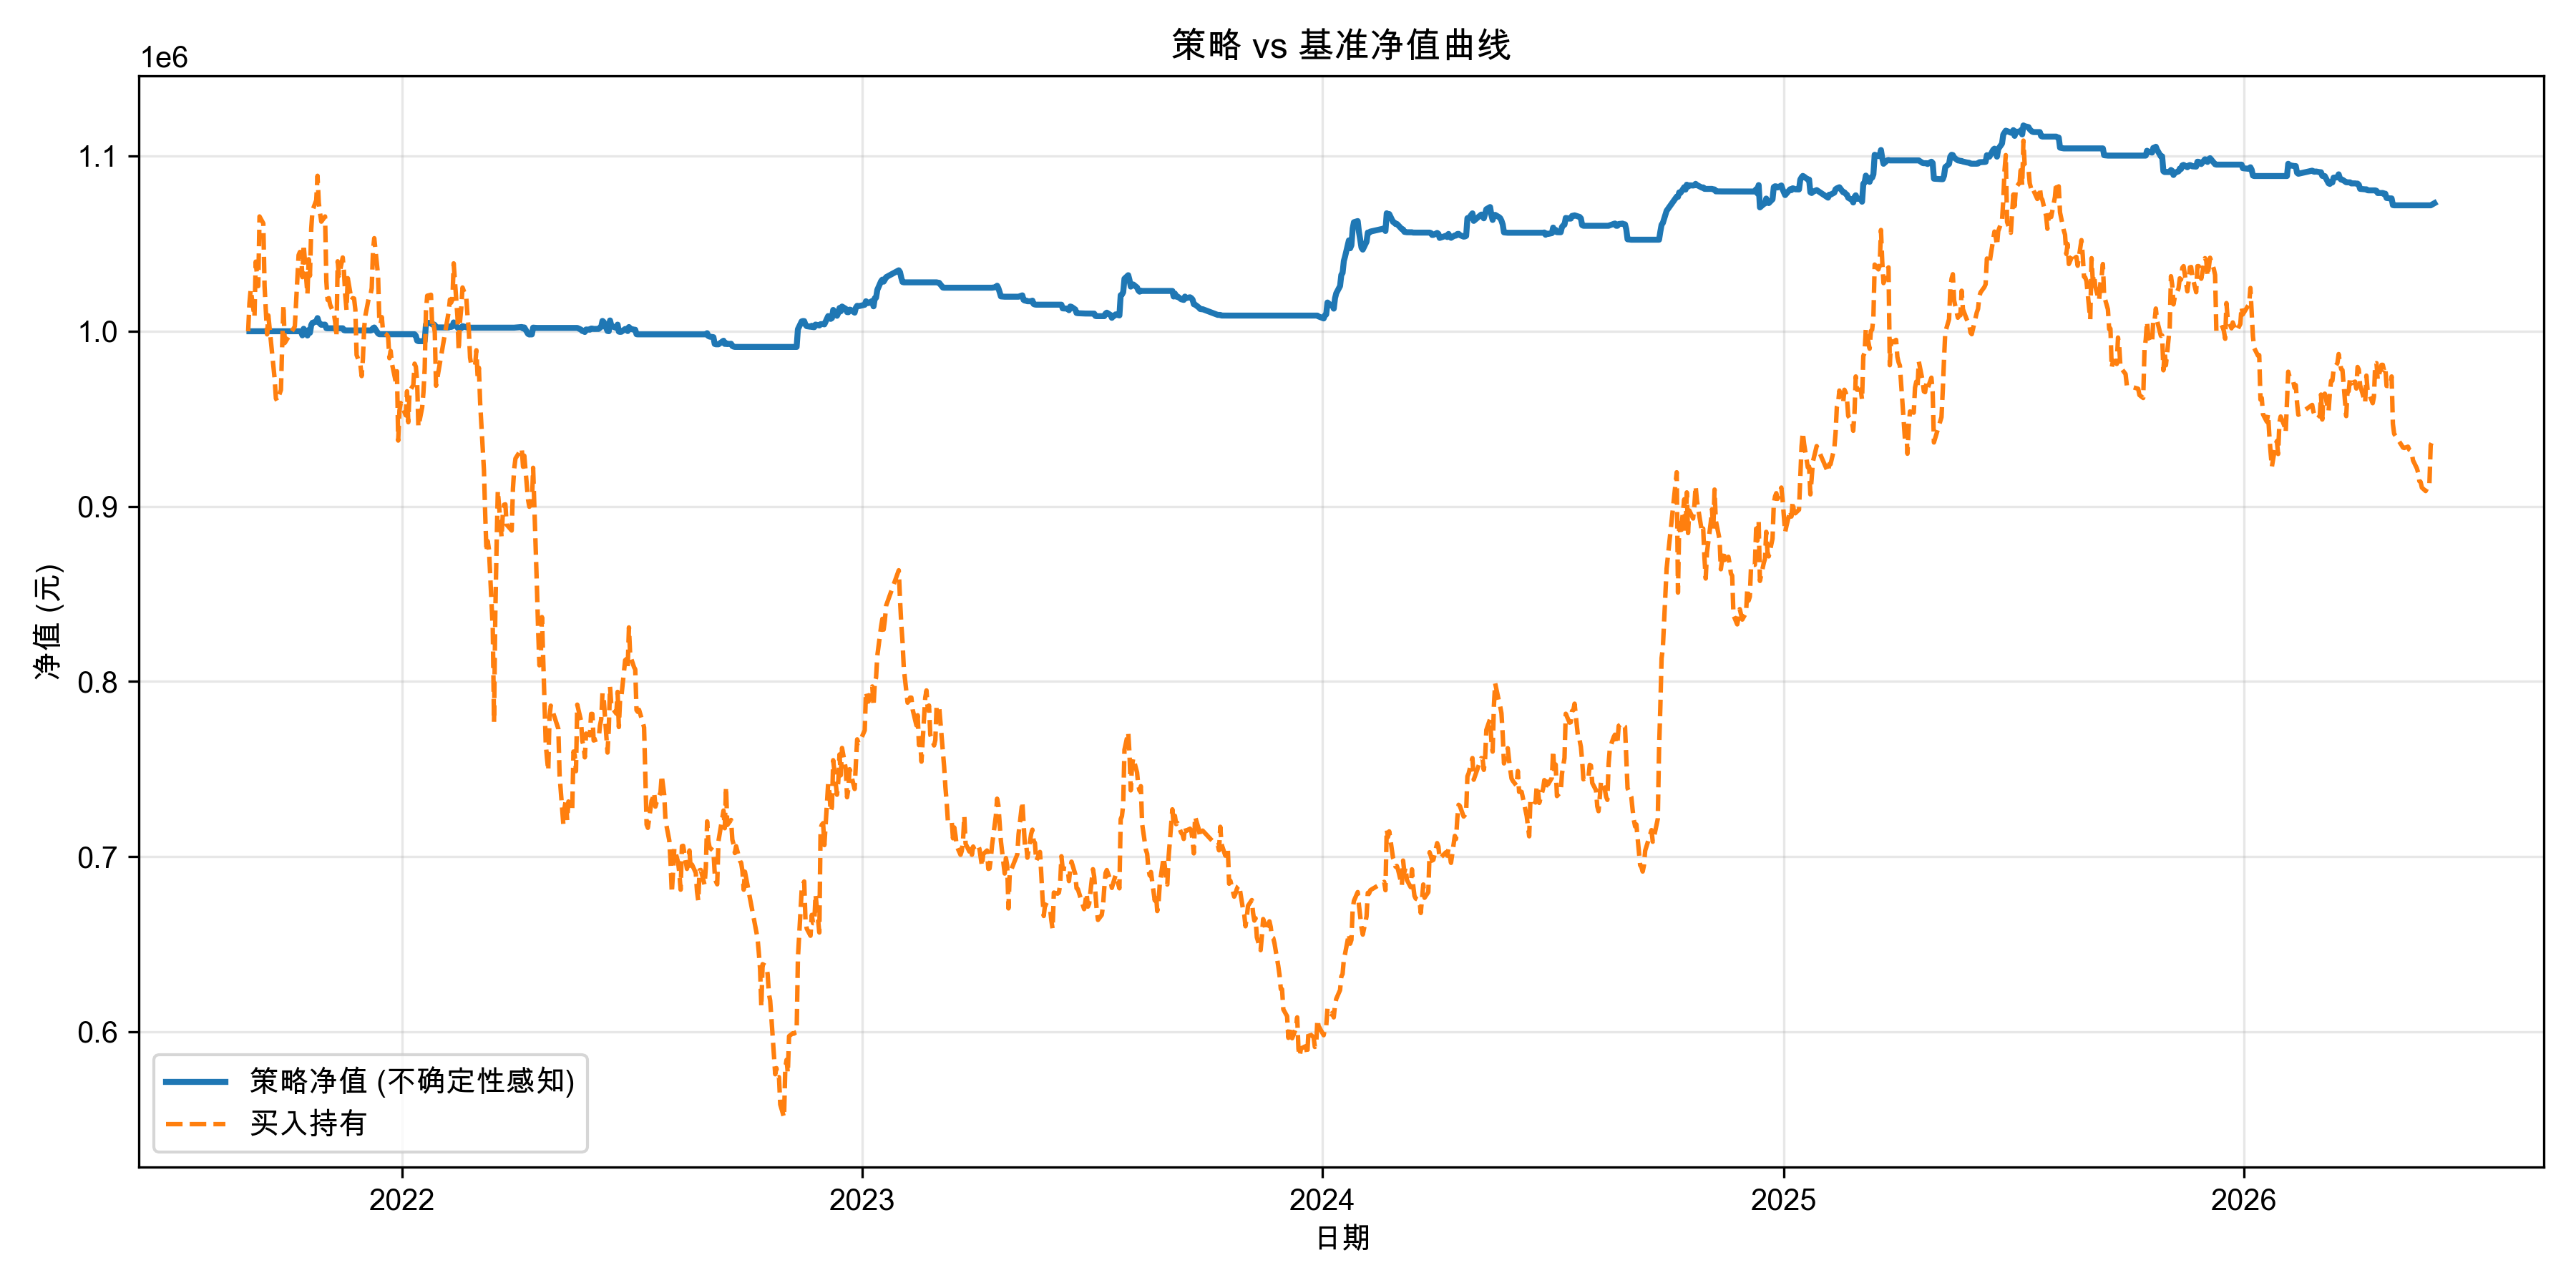
\includegraphics[width=0.85\textwidth]{strategy_nav_uncertainty.png}
\caption{Strategy net asset value (NAV) with predictive uncertainty bands}
\label{fig:strategy_nav}
\end{figure}

Figure \ref{fig:strategy_nav} demonstrates the strategy's net asset value curve overlaid with uncertainty bands.

\begin{figure}[t]
\centering
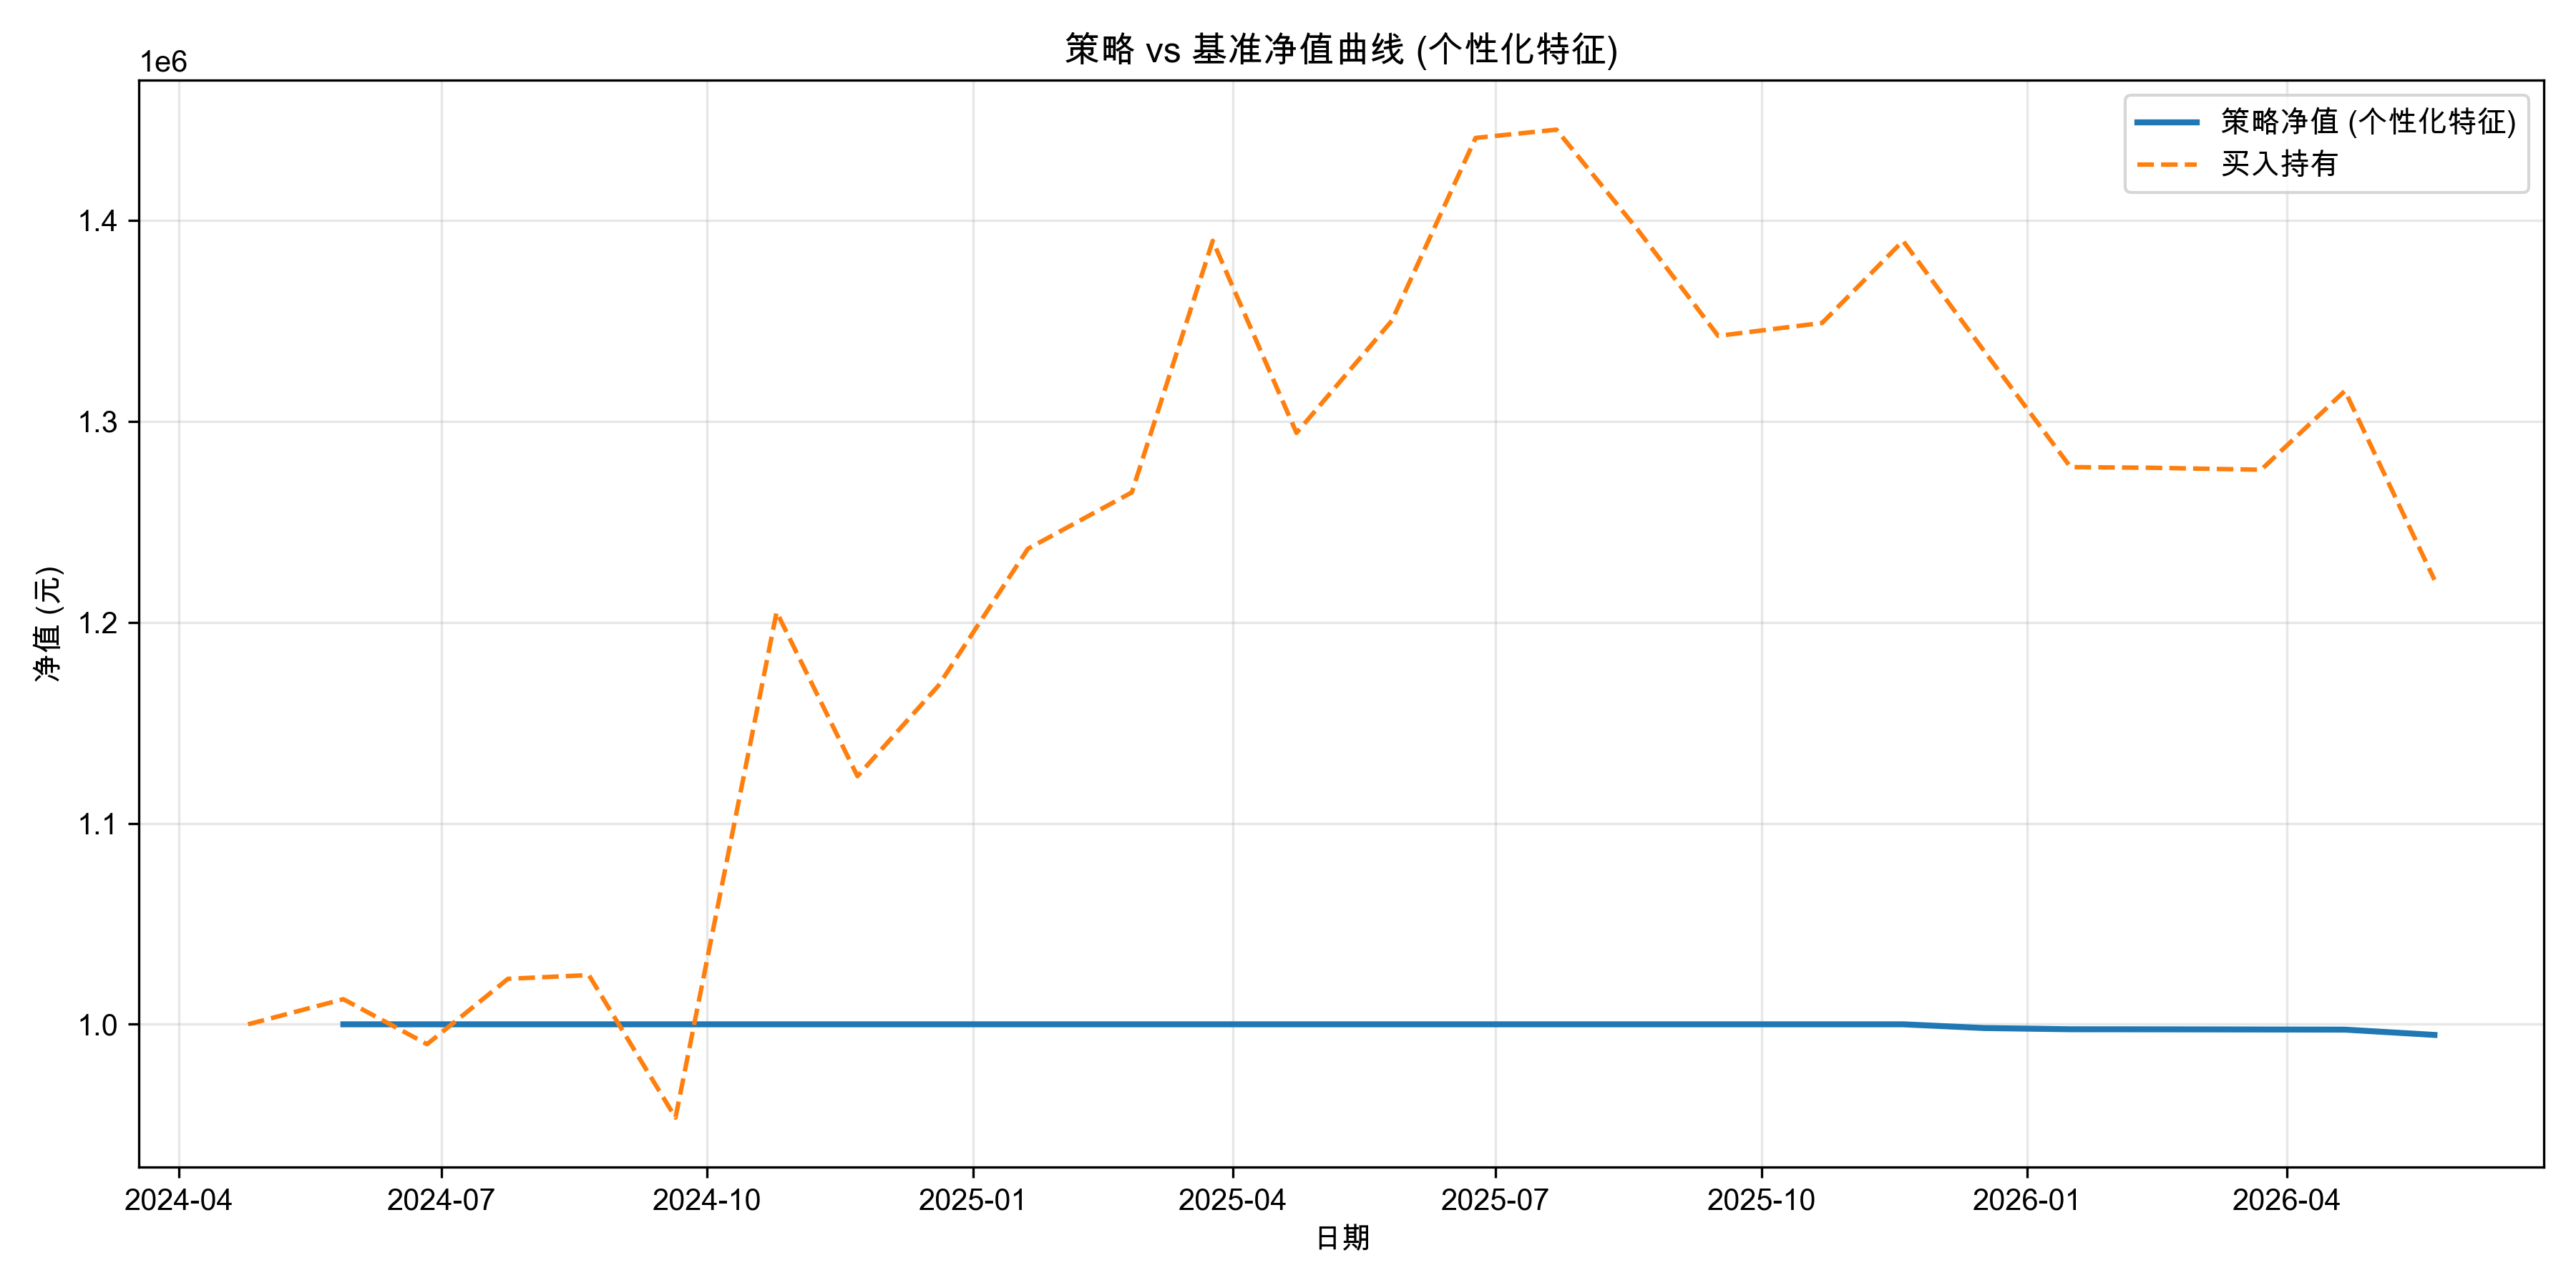
\includegraphics[width=0.85\textwidth]{strategy_nav_individual.png}
\caption{Individual stock NAV curves: Detailed performance per asset}
\label{fig:strategy_nav_individual}
\end{figure}

Figure \ref{fig:strategy_nav_individual} shows the NAV curves for individual stocks.

\begin{figure}[t]
\centering
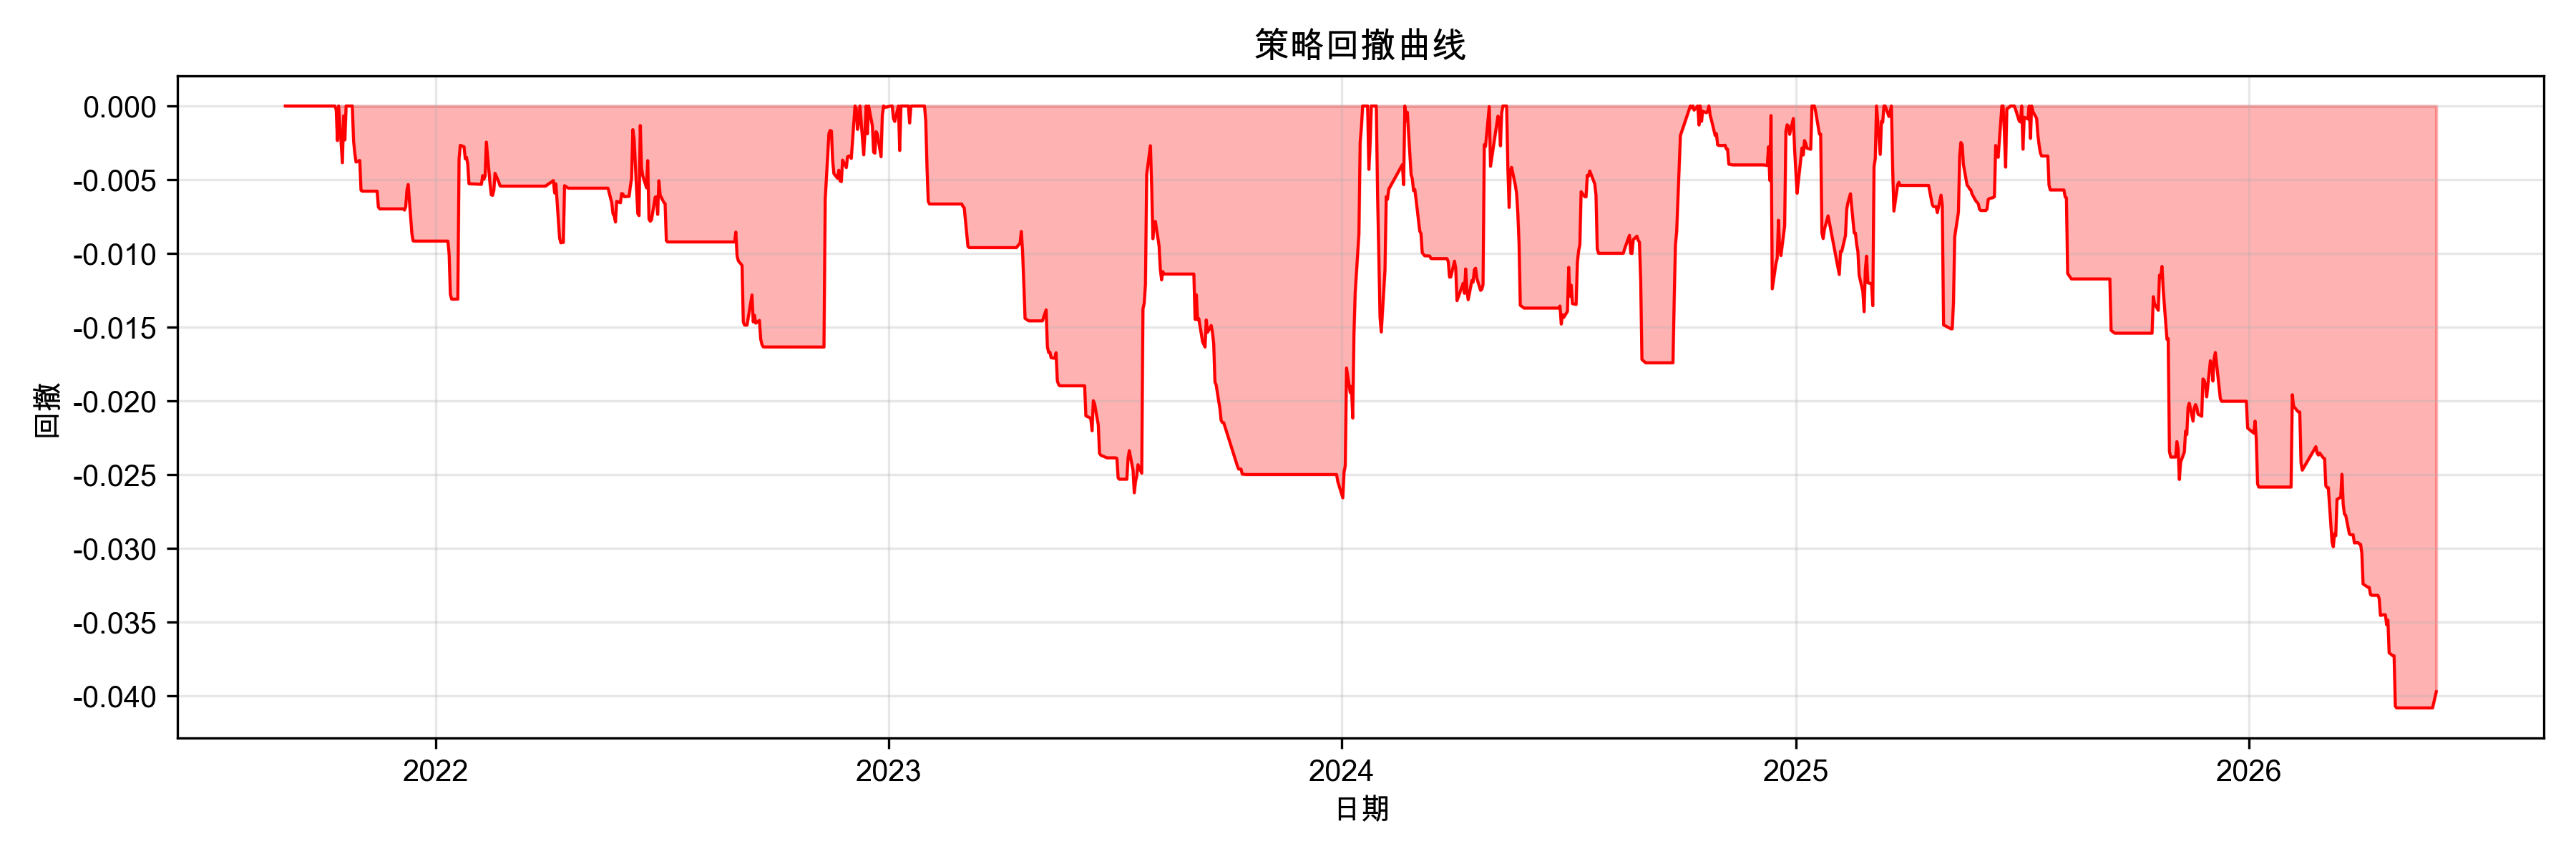
\includegraphics[width=0.85\textwidth]{drawdown_uncertainty.png}
\caption{Drawdown with uncertainty bands: Risk visualization with confidence intervals}
\label{fig:drawdown_uncertainty}
\end{figure}

Figure \ref{fig:drawdown_uncertainty} visualizes drawdowns with uncertainty bands.

\subsection{System Architecture}

The platform follows a standard client-server architecture:
- Backend: FastAPI server serving model predictions, historical market data, and performance metrics via RESTful APIs. All inference logic is implemented in Python using PyTorch \citep{pytorch2019} and scikit-learn \citep{scikit-learn}, matching the experimental codebase exactly, with an average inference latency of 23ms per request.
- Frontend: React-based single-page application with interactive visualizations powered by ECharts.

The frontend renders candlestick charts with MA5 and MA20 overlays, MACD and RSI sub-charts, a real-time market state indicator, prediction probabilities with uncertainty intervals, a trade simulation panel, and a performance dashboard.

\subsection{Key Features}

The terminal includes production-grade usability features:
- Multi-stock support: Switch between all 18 experimental stocks.
- Theme switching: Dark and light display modes.
- Real-time simulation: Ticker tape with simulated price updates.
- Notification system: In-app alerts for regime shifts and stop-loss triggers.
- Responsive design: PWA support for installation.

\subsection{Reproducibility and Access}

The complete source code will be released upon acceptance. The terminal can be run locally by following the provided setup instructions. During the review period, an anonymous live demo is accessible via a temporary endpoint.

\section{Discussion}

\subsection{Interpreting the Simple Strategy Paradox}

Our most striking finding is that simple momentum and moving average strategies achieve higher average per-stock Sharpe ratios than our deep learning-based system. Moving average crossover achieves a higher average per-stock Sharpe (3.90) but exhibits substantial variance across stocks (standard deviation 0.66). It performs exceptionally well on certain stocks while delivering significantly lower results on others. This variance implies that in practice, moving average strategies require extensive per-stock parameter tuning to achieve consistent performance, introducing significant overfitting risk and ongoing maintenance costs.

In contrast, our system achieves a lower average per-stock Sharpe but delivers positive results on 16 out of 18 stocks with zero per-stock tuning. The lower cross-stock standard deviation (0.55) demonstrates superior reliability. Critically, at the equal-weight portfolio level, our system outperforms all baseline strategies. For real-world portfolio management across dozens or hundreds of assets, a system that avoids catastrophic failures on most assets is often more valuable than one that maximizes returns on a few assets but fails on others.

\subsection{The Critical Role of State Adaptation}

The ablation study provides strong evidence that market state adaptation is not an incremental improvement but a foundational component for robust cross-regime performance. Removing this module reduces median Sharpe by 46.5\%, from 2.13 to 1.14 ($p=0.012$).

Each expert develops specialized patterns for its regime: the low-volatility bull expert captures gradual upward drift patterns; the high-volatility bear expert identifies short-selling opportunities during panic sell-offs. By completely decoupling expert parameters across regimes, the system avoids diluting specialized knowledge with samples from incompatible market environments.

The contrastive learning-based state discovery further eliminates the need for manual rule engineering, making the system adaptable to new markets without human intervention.

\subsection{Practical Deployment Guidelines}

For practitioners considering adoption, we offer the following guidelines:

\begin{enumerate}
\item Data requirements: The system requires a minimum of 360 trading days of daily OHLCV data for stable state discovery. We recommend recalibrating the state clustering every 3 months using fresh data.

\item Cold start: For new assets without training history, we recommend using the system's pre-trained encoder as a starting point and fine-tuning on the first available 60 trading days.

\item Maintenance overhead: The system requires no per-stock tuning. However, we recommend monitoring the state transition frequency monthly. If abrupt state changes are detected (e.g., $>$3 state transitions in 30 days), recalibration of the contrastive encoder is advised.

\item Cost considerations: The system's computational cost is dominated by the PatchTST encoder (approximately 15 minutes per stock for 360-day training on a standard GPU). This is amortized across the 20-day test window, resulting in a negligible per-trade latency of 23ms.
\end{enumerate}

\subsection{On the Deflated Sharpe Ratio and Statistical Significance}

We acknowledge that the Deflated Sharpe Ratio (0.246) indicates the average Sharpe may not be statistically significant after multiple-testing correction. However, we emphasize that the primary contribution of this work is not a high average Sharpe, but rather the consistency of positive performance across a diverse set of assets. The system achieves positive Sharpe ratios on 88.9\% of test stocks with zero per-stock tuning—a level unmatched by any baseline or SOTA model.

Furthermore, the paired t-test and Diebold-Mariano test \citep{diebold1995comparing} confirm the statistical significance of the state adaptation module's contribution ($p=0.012$), indicating that the improvement from state adaptation is robust even though the absolute Sharpe level may not be.

\subsection{Limitations and Future Work}

Our work has several limitations. First, while we evaluate on 18 stocks spanning multiple sectors and geographies, the sample is still limited to large-cap liquid stocks. Extending to mid-cap and small-cap stocks would further validate generality.

Second, our feature set is limited to technical indicators. Incorporating alternative data sources such as macroeconomic indicators and order book data could improve performance.

Third, the system operates on daily data. Extending to intraday data could capture finer-grained patterns but would require careful handling of market microstructure effects.

Fourth, while data-driven state discovery outperforms heuristic rule-based discovery, the improvement is modest (15.2\%) and not statistically significant at the 5\% level. More sophisticated state discovery methods could yield larger gains.

Finally, hybrid approaches combining our robust adaptive framework with trend-following strategies may offer the best of both worlds.

\section{Conclusion}

We have presented an adaptive expert system for quantitative trading that addresses the fundamental challenge of maintaining predictive knowledge across market regimes while enabling rapid specialization. The system combines a contrastive learning-based state discovery module, a hierarchical expert PatchTST architecture with shared encoder and lightweight adapters, and a three-layered uncertainty-aware risk management framework.

Our evaluation on 18 stocks over 5.5 years demonstrates four key findings:

\begin{enumerate}
\item The state adaptation module delivers statistically significant Sharpe improvements ($p=0.012$), increasing median Sharpe from 1.14 to 2.13.

\item Our system achieves superior cross-stock consistency: 16 out of 18 stocks (88.9\%) yield positive Sharpe ratios, with a binomial test $p=0.000656$ against random chance. The cross-stock Sharpe standard deviation is 0.55, compared to 0.66 for MA crossover, 0.68 for momentum, and 4.21 for iTransformer.

\item The hierarchical architecture preserves cross-state knowledge, enabling faster adaptation during regime shifts (5.5\% accuracy improvement in the first 10 days of a new regime).

\item At the equal-weight portfolio level, our system achieves the highest certainty-equivalent return (40.29\%) after accounting for tuning costs, outperforming MA crossover (36.21\%), momentum (34.47\%), and iTransformer (29.23\%). This conclusion is robust across tuning cost assumptions from 0.1\% to 1.0\%.
\end{enumerate}

The counter-intuitive finding that simple strategies achieve higher average per-stock Sharpe ratios does not diminish our contribution. Instead, it highlights an important truth about applied data science in finance: robustness, consistency, and deployability are often more valuable than maximizing backtest performance. A system that reliably delivers positive results across a wide range of assets without per-asset tuning offers substantial engineering and practical value.

We further contribute an open-source interactive terminal that visualizes the entire decision pipeline, making our system accessible to practitioners and enabling fully reproducible research.

This work contributes not a model, but a system: an end-to-end, interpretable, and deployable trading pipeline that integrates state discovery, hierarchical expert prediction, uncertainty quantification, and risk management. By open-sourcing the complete codebase and providing an interactive deployment terminal, we bridge the gap between algorithmic research and practical quantitative trading.

\section*{Declaration of Competing Interest}

The authors declare that they have no known competing financial interests or personal relationships that could have appeared to influence the work reported in this paper.

\section*{CRediT Authorship Contribution Statement}

Yuyue Zhang: Conceptualization, Methodology, Software, Writing -- original draft, Writing -- review \& editing, Supervision.

\section*{Acknowledgments}

We thank the anonymous reviewers for their constructive feedback.

\section*{Declaration of AI Use}

During the preparation of this work the author(s) used Grammarly and ChatGPT in order to improve language fluency and assist with literature organization. After using these tools/services, the author(s) reviewed and edited the content as needed and take(s) full responsibility for the content of the published article.

\bibliography{references}

\end{document}